\documentclass[UTF8,a4paper]{ctexart}
\usepackage[margin=1in]{geometry}
\usepackage{fancyhdr,hyperref,float,graphicx,color,amsmath}
\pagestyle{fancy}
\hypersetup{hidelinks}
\pdfminorversion=5 
\pdfcompresslevel=9
\pdfobjcompresslevel=2
\lhead{\bfseries \leftmark}
\chead{}
\rhead{SCUT}
\lfoot{\url{https://github.com/285571052}}
\cfoot{qhy}
\rfoot{\thepage}
\setlength{\headheight}{13pt}
\renewcommand{\headrulewidth}{0.4pt}
\renewcommand{\footrulewidth}{0.4pt}

\setlength{\parindent}{0pt}
\newcommand{\spaceline}{\vspace{\baselineskip}}

\author{ qhy }
\date{\today}
\title{操作系统}

\begin{document}
\maketitle
\tableofcontents
\newpage

\section{介绍}

\paragraph{什么是操作系统?}操作系统是一个运行在内核态的软件 , 为用户提供良好的用户接口;操作系统是一个资源管理器,对多进程以及资源(共享)进行控制

\paragraph{CPU的状态:核心态(也叫管态)、用户态(也叫目态)他们的特征是什么?}
\begin{itemize}
	\item 内核态 : 操作系统具有对所有硬件的完全访问权, 可以执行机器能够运行的任何指令
	\item 用户态 : 只使用了机器指令的一个子集 , 特别是那些会影响机器的控制或可进行I/O操作的指令在用户态是被禁止的
\end{itemize}

\paragraph{系统调用的过程}
\begin{figure}[H]
	\centering
	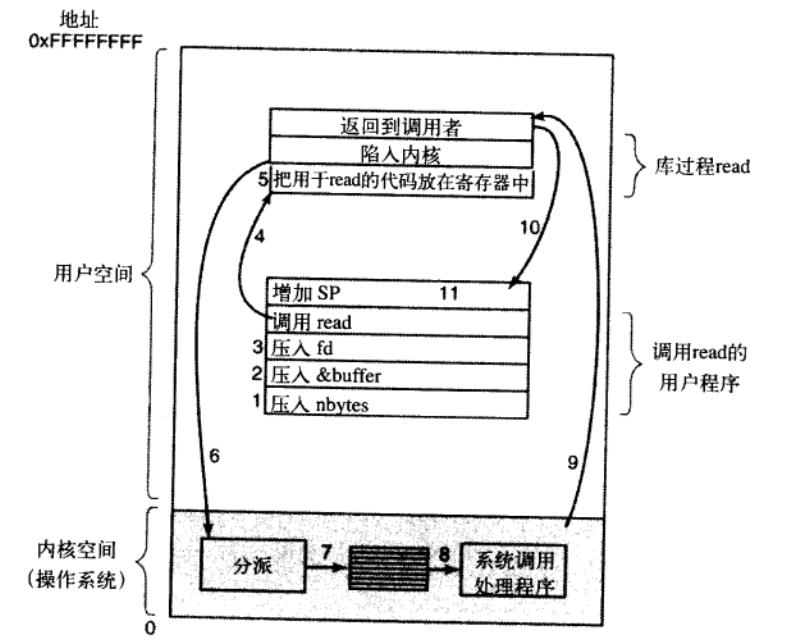
\includegraphics[scale = 0.3]{assets/ModernOperatingSystems/2018-01-11-19-44-54.png}
	\caption{完成系统调用read的11个步骤}
\end{figure}

\paragraph{过程调用和系统调用的区别}
\begin{itemize}
	\item 系统调用需要切换到内核态和过程调用指令并不改变模式
	\item 过程调用可以给定任意的绝对或相对路径的任意地址, 而系统调用只能跳转到一些指定的地址
\end{itemize}

\paragraph{操作系统结构} 单体系统 ;层次式系统 ; 微内核 ; 客户机-服务器模式 ;虚拟机 ; 外核

操作系统的特征:虚拟性(Virtualization)、并发性(concurrency)、异步性、共享性和持久性(persistency)

\section{进程}
%{\color{blue}分三次课讲}
\subsection{进程的创建与终止}

\textbf{进程的创建时间:}
\begin{itemize}
	\item 系统启动,reboot
	\item 命令行或打开图标
	\item fork(),创建子进程
	\item 启动一个批处理(batch job)
\end{itemize}

{\color{blue}命令行后面加个$\&$ 表示后台运行}

\spaceline
\textbf{进程的终止:}
\begin{itemize}
	\item 正常退出,Normal exit\\
	      end of main
	\item 错误终止 error exit\\
	      exit(2)
	\item 致命错误,Fatal error\\
	      除0等
	\item 被终止,kill by another process\\
	      kill pid
\end{itemize}

\textbf{用户与程序的关系:}
用户启动程序,有两种情况:
\begin{itemize}
	\item 多个用户启动多个程序
	\item 多个用户共享一个实例
\end{itemize}

% \textbf{实例:}一个实例对应一个进程 , 一个进程可以对应多个程序。

{\color{blue}查看进程:
\begin{itemize}
	\item Linux\\
	      ps -e
	\item Windows\\
	      ctrl + alt + delete
\end{itemize}}

\subsection{进程模型}
主要有两种分类:
\begin{itemize}
	\item 多进程,串行运行
	\item 多进程,并行运行\\
	      实际上是多个进程交替运行一段时间,在单处理器机器上,本质上还是串行运行
	      ,即某个时间点只有一个程序运行(分时运行)
\end{itemize}

\textbf{进程的层次结构:}父进程可以创建子进程,子进程也可以创建它的子进程。

若一堆进程有同一个父进程,则称为进程组。

进程的状态:
\begin{figure}[H]
	\centering
	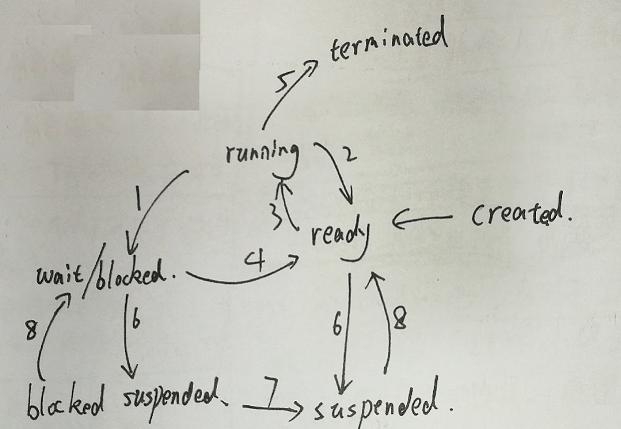
\includegraphics[scale = 0.3]{assets/caozuoxitong_fe21f.png}
	\caption{进程的状态}
\end{figure}
\begin{figure}[H]
	\centering
	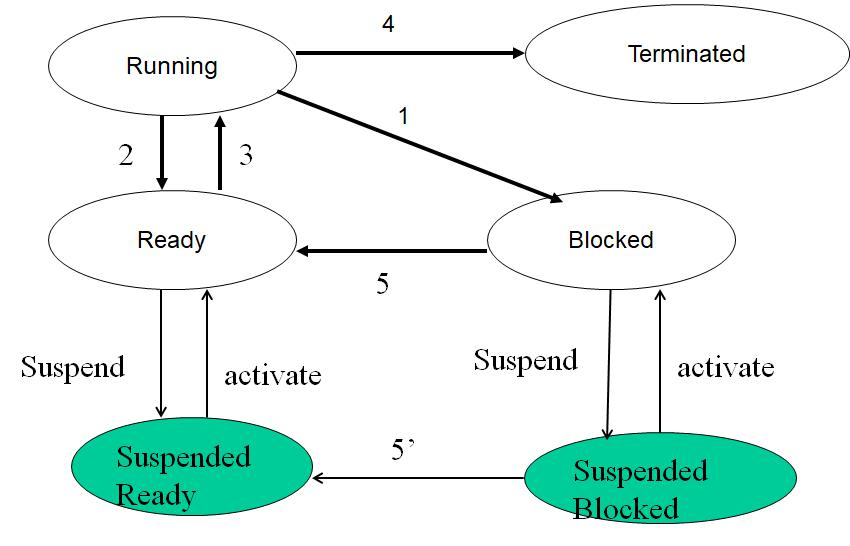
\includegraphics[scale = 0.3]{assets/ModernOperatingSystems_ef0b3.png}
\end{figure}

\begin{itemize}
	\item [0.] 创建进程
	\item [1.] 阻塞状态\\
	      等待非CPU资源的申请,如I/O的申请
	\item [2.] 停止运行当前进程,运行其他进程
	\item [3.] 运行当前程序
	\item [4.] 一切准备就绪(申请得到资源等),等待运行(等待CPU时间分配)
	\item [5.] 进程终止
	\item [6.] 进程挂起\\
	      (当内存紧张时)先把进程非运行着的进程放一边去
	\item [7.] 等待的设备已经可用,不会直接进入ready而是进入suspended
	\item [8.] 唤醒

\end{itemize}

\subsection{进程的实现}
\textbf{进程是什么?}进程是一个程序运行着的实例 ,它和其他实例唯一区分 , 能创建其他进程 , 或者被其他进程所创建

每个进程都有各自的地址空间 , 因此 , 每个进程的地址相同 ,但值不一样(实现 : 内存映射)

\subsection{地址空间}
一般情况,内核空间的地址较大,而用户空间的地址较小。比如
% \begin{tabular}{|c|}
%   \hline\\
%   $0xFFFF\cdots$内核空间\\
%   $stack$\\
%   $\cdots$\\
%   $heap$\\
%   $0x0000\cdots$用户空间(code和data)\\
%   \hline
% \end{tabular}
\begin{figure}[H]
	\centering
	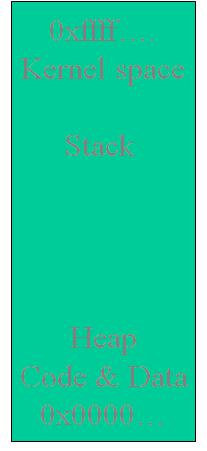
\includegraphics[scale = 0.3]{assets/ModernOperatingSystems_8866a.png}
	\caption{内核空间的地址大,用户空间地址小}
\end{figure}
即,用户代码与数据 和 内核代码 分别放在地址空间两端,而堆和栈则放在次两端, 这样就能保证堆和栈在增长的时候
有空间可以用,而无需拷贝移动到更大的地址空间中。

\spaceline
\subsection{程序区段}
进程由两个部分组成 : \textbf{程序区段} 和 \textbf{进程控制块}

\textbf{程序区段}
\begin{itemize}
	\item Text
	\item Data
	\item Stack
	\item Heap
\end{itemize}

\subsection{进程控制块(Process Control Block ,PCB)}

\textbf{PCB:}记录进程相关的信息,见图\ref{fig-PCB}

\begin{figure}[H]
	\centering
	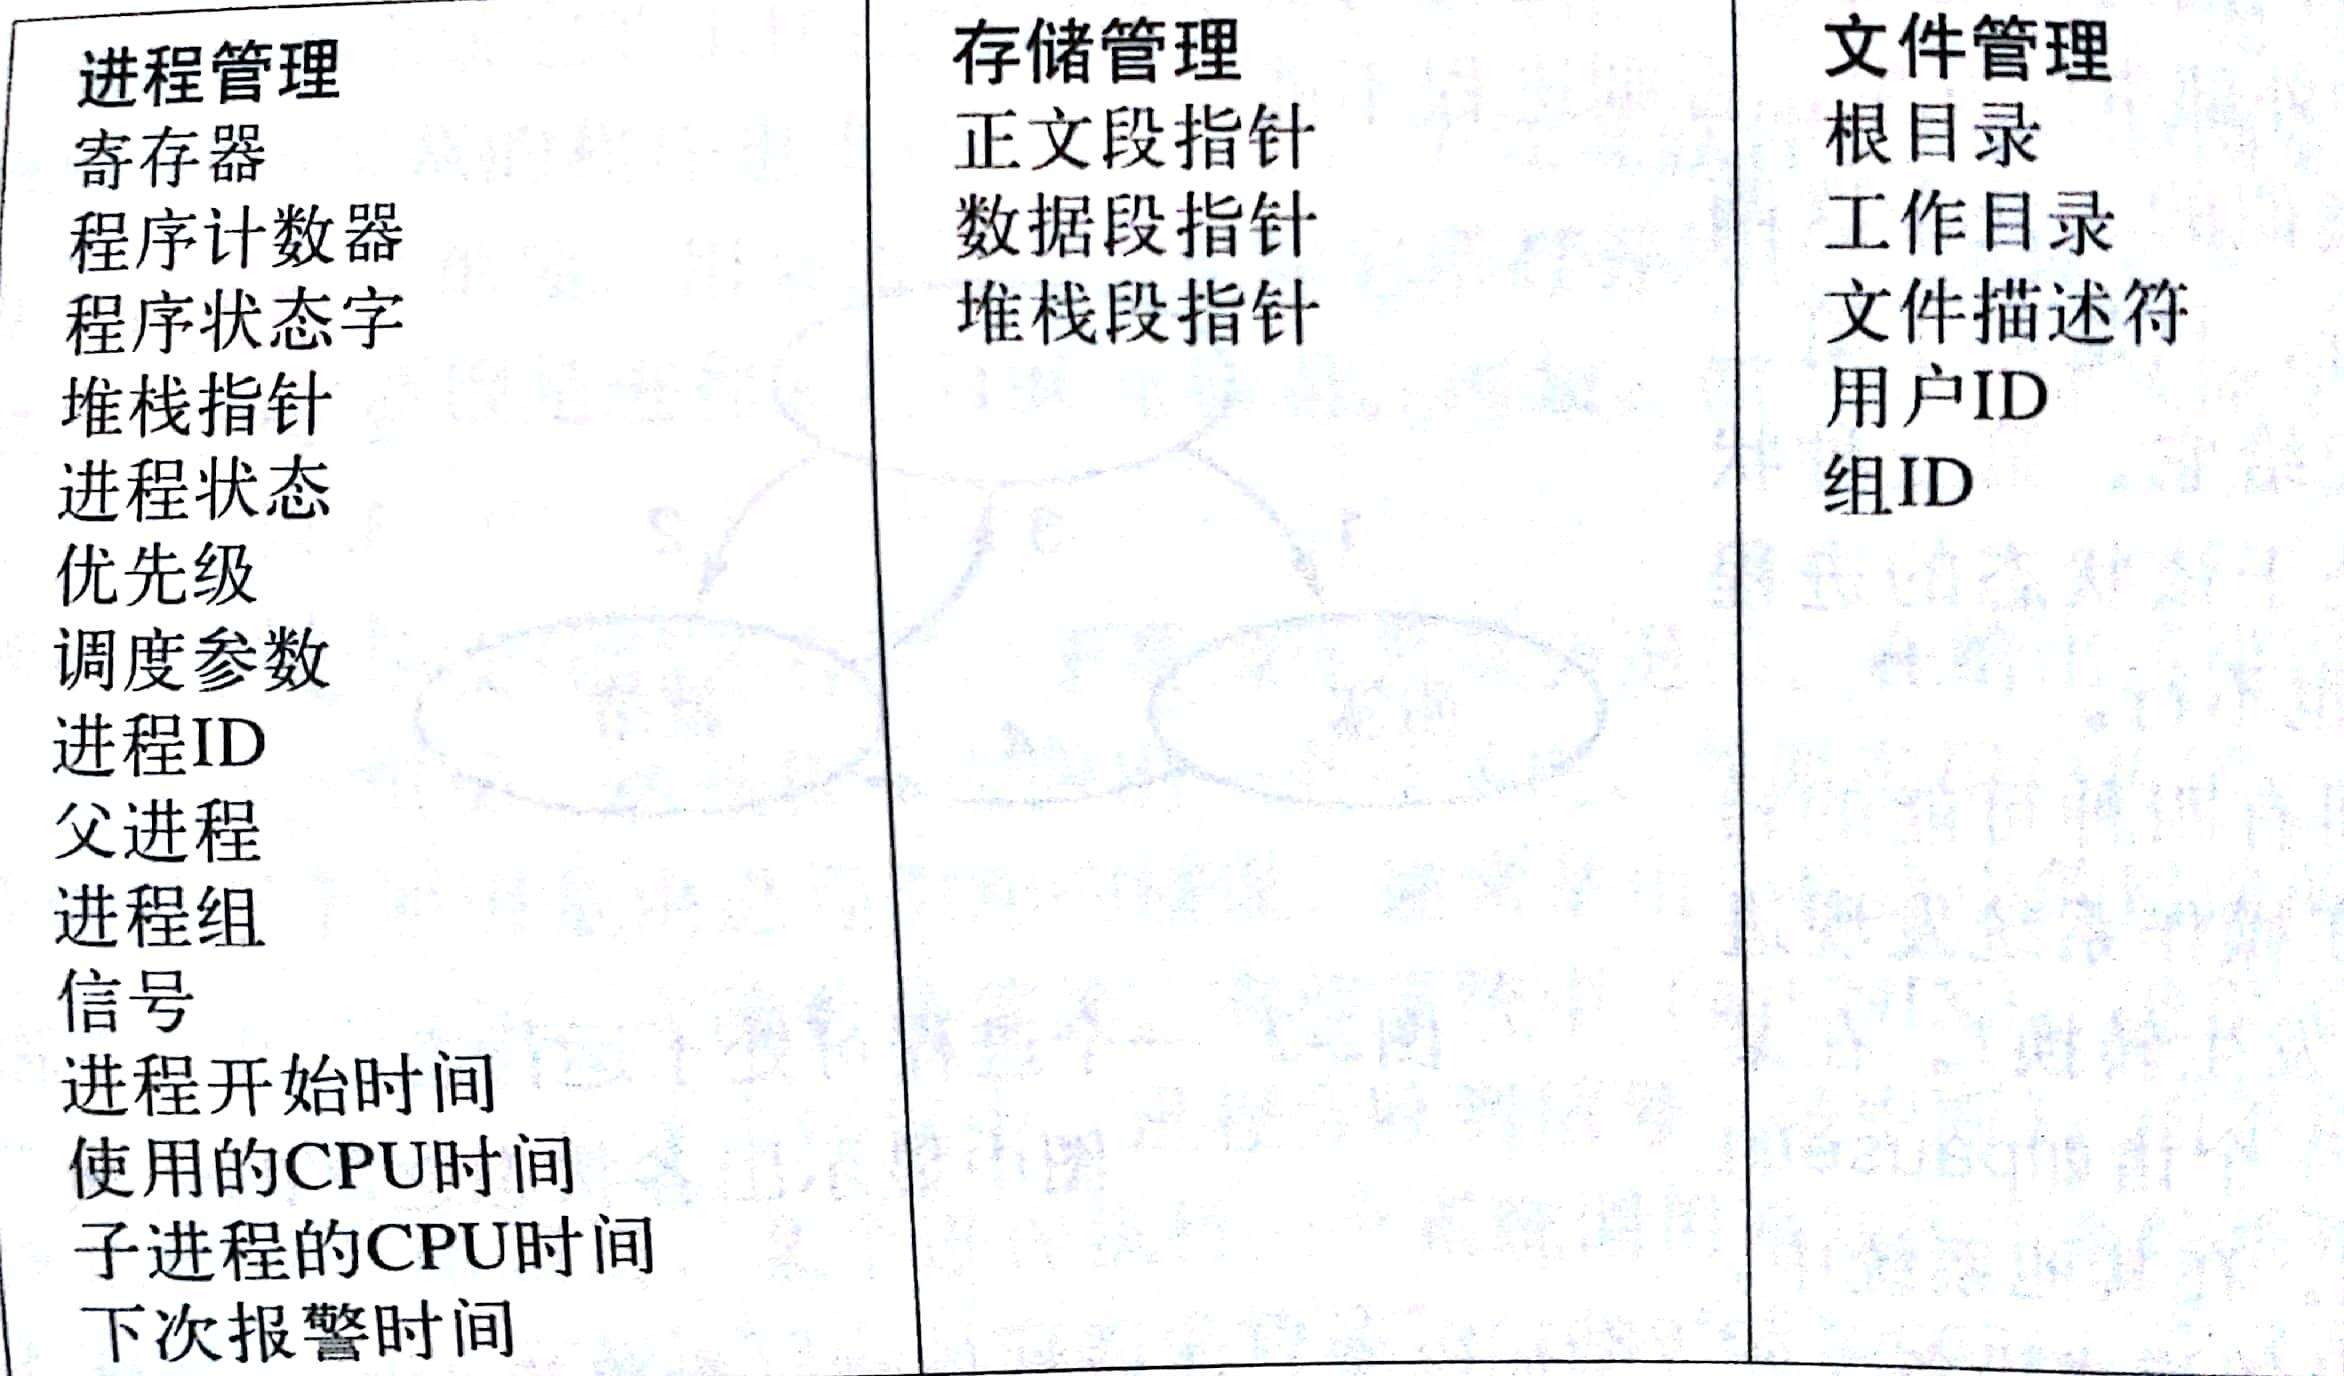
\includegraphics[scale = 0.1]{assets/ModernOperatingSystems_e6663.png}
	\caption{Process Control Block}
\end{figure}

\subsection{上下文切换 Context Switch}
\textbf{上下文切换}:切换CPU的进程,主要分为以下几个步骤。
\begin{itemize}
	\item 保存旧进程的PCB
	\item 载入新进程的PCB
	\item 刷新缓存Cache
	\item 改变内存映射表(TLB)
\end{itemize}

上下文切换由进程调度负责完成 , 并且时间代价很大(1-1000ms) , 同时需要硬件支持

\textbf{CPU利用率:}直接定义是$\displaystyle{
	 \frac{\text{CPU有效时间}}{\text{CPU总时间}}}
$,$1 - p^n$,其中$p$为一个进程等待$I/O$的时间与其停留在内存时间的比,n为同在内存的进程数。

{这个n次方怎么理解?计算所有CPU都在等待的时间比例 , p表示一个进程没有利用到CPU的时间的比例, 但是这个比例中,有部分是被其他进程所使用的
,因此再乘上其他进程没用到的比例才是CPU总体没被利用的比例,这里去了近似,所有的进程未利用的比例都是p,因此是$p^n$}

\section{线程 Thread}
\textbf{线程:}
\begin{itemize}
	\item 线程是轻量级进程 Lightweight Process
	\item 一个进程可以同时做多件事情
	\item 同进程的线程可以共享进程内的相同资源
	\item 每个线程都有自己的栈空间\\
	      因为并行处理,栈空间是不能共享的,否则会发生冲突。\\
	      那么问题来了,栈到底是怎么实现的?其实就是取一块内存块作为栈空间,因此栈的大小并不是无限大的,而是有限制的
	      ,这也是为什么会存在爆栈的现象。
\end{itemize}

\begin{figure}[H]
	\centering
	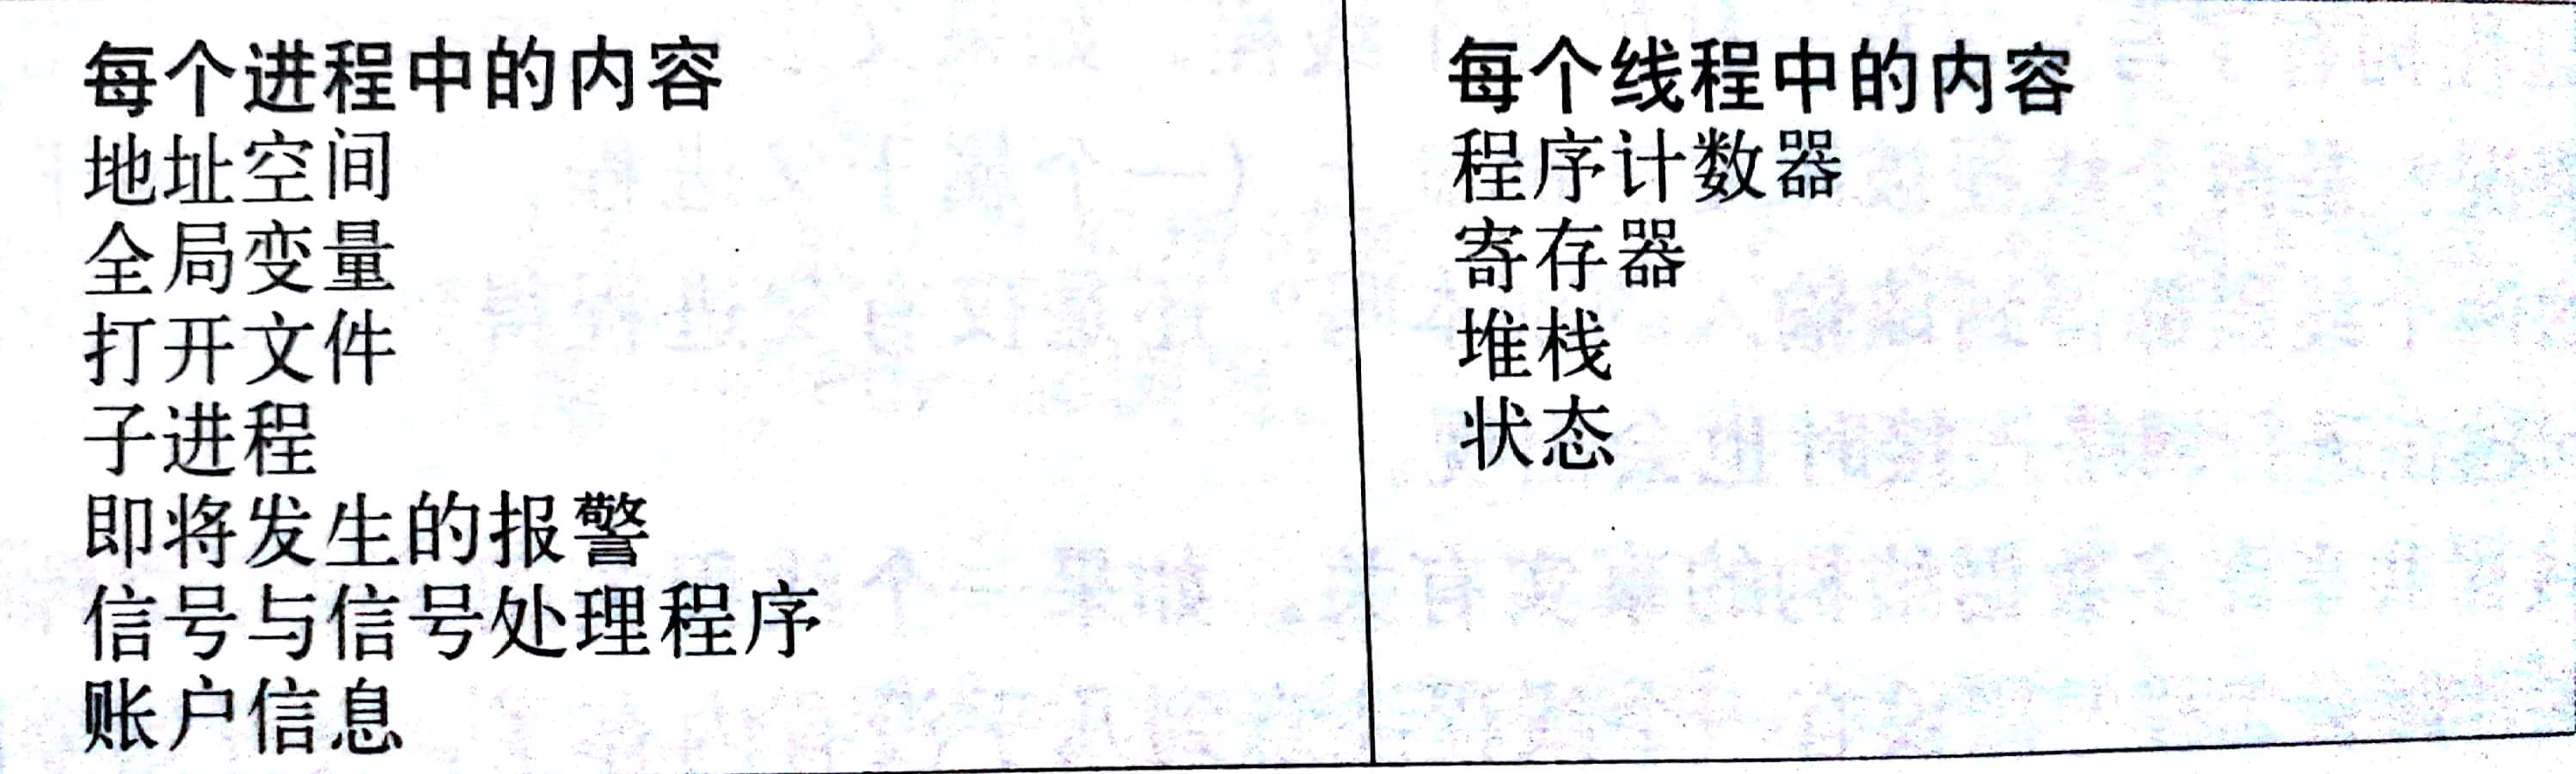
\includegraphics[scale = 0.1]{assets/ModernOperatingSystems_8204b.png}
	\caption{进程中所有线程共享的内容 与 每个线程自己的内容}
\end{figure}

\textbf{POSIX线程标准:}某个线程标准,在C中使用\textbf{pthread.h}调用相关函数。

\subsection{线程的实现方式}

\textbf{线程的实现方式:}
\begin{itemize}
	\item 在用户空间中实现线程(Old linux)\\
	      即线程表放在用户空间中,调用一个进程,运行的是线程。\\
	      内核对线程一无所知。
	      \begin{figure}[H]
		      \centering
		      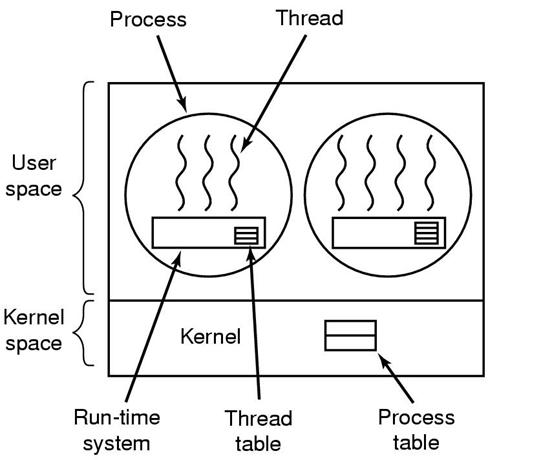
\includegraphics[scale = 0.3]{assets/ModernOperatingSystems_df08d.png}
	      \end{figure}
	\item 在内核空间中实现(Windows XP/2000)\\
	      即线程表放在内核中,由内核来管理线程。
	      \begin{figure}[H]
		      \centering
		      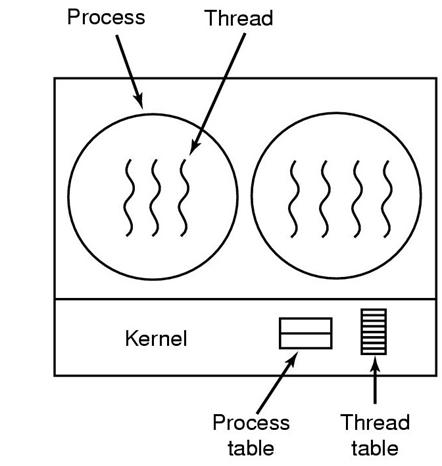
\includegraphics[scale = 0.3]{assets/ModernOperatingSystems_d3de3.png}
	      \end{figure}
	\item 上面两种的混合型(Solaris)\\
	      用户级线程与内核线程多路复用。\\
	      一个内核线程可以对应多个用户线程。一个内核线程回被多个用户级线程多路复用
	      \begin{figure}[H]
		      \centering
		      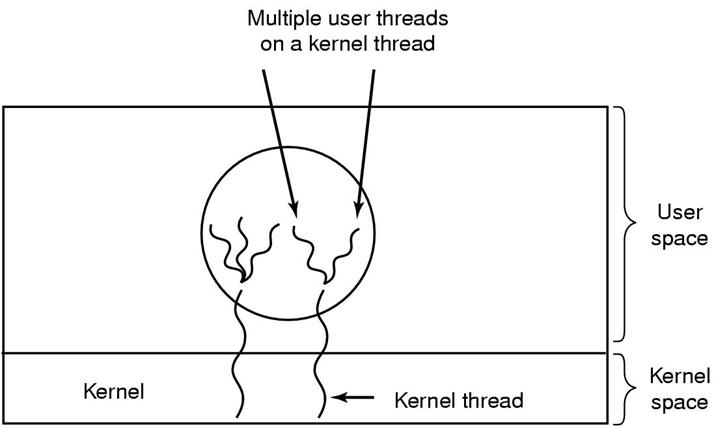
\includegraphics[scale = 0.3]{assets/ModernOperatingSystems_416b1.png}
	      \end{figure}
\end{itemize}

\subsection{调度程序激活机制}

\textbf{调度程序激活机制:}尽管内核级线程在一个关键点上优于用户级线程,但是内核线程速度慢,因此采用调度程序激活机制来
保持优良特性的情况下改进速度。

调度程序激活工作的目标是模拟内核线程的功能 , 但是为线程包提供通常在用户空间才能实现的更好的性能和更大的灵活性

当使用调度程序激活机制时 , 内核给每个进程安排一定数量的虚拟处理器, 并且让(用户空间)运行时系统将线程分配到处理器上
% {\color{red}内核级线程有什么优良特性?后面再补充这一方面的内容。}

% \spaceline
\subsection{弹出式线程}
\begin{figure}[H]
	\centering
	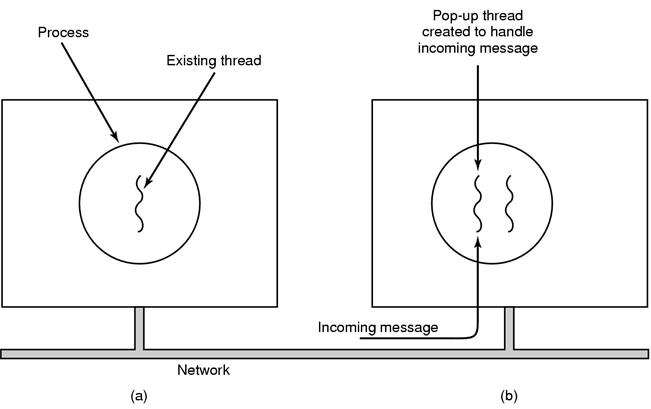
\includegraphics[scale = 0.3]{assets/ModernOperatingSystems_6789a.png}
	\caption{弹出式线程}
\end{figure}
\textbf{弹出式线程}: 当一个消息到达系统时,创建一个处理该消息的线程

由于没有历史信息 , 那么就没有必须存储的寄存器 , 堆栈等内容 , 就可以快速的创建以线程 , 由于快速创建 , 消息到达与处理器之间的时间非常短

% \spaceline
% \textbf{作业:P95-97 , 1 , 6 ,7 11,12}

\section{调度}

\subsection{为什么需要调度}
当计算机系统是多道程序设计系统时,通常就会有多个进程或线程同时竞争 CPU ,只要有两个或更多的进程处于就绪
状态,这种情形就会发生。如果只有一个CPU可用,那么久必须选择下一个要运行的进程。在操作系统中,完成选择工作
的一部分就称为\textbf{调度程序(scheduler)},该程序使用的算法称为\textbf{调度算法(scheduling algorithm)}

\spaceline
\textbf{何时调度?执行调度程序的时机?}
\begin{itemize}
	\item 进程创建/终止
	\item I/O中断
	\item 运行中的进程被阻塞
	\item 时钟中断
\end{itemize}

\textbf{抢占式调度与非抢占式调度:}
\begin{itemize}
	\item 抢占式调度:运行着的进程被强制放弃使用CPU(非当前运行着的进程控制)\\
	      抢占主要体现在CPU选择下一个任务的时候,某些任务优先占有的CPU。\\
	      分为两个阶段,首先是运行程序被强行中断至就绪状态(或者运行程序运行完毕或阻塞),\\
	      然后优先级\footnote{优先级:这里的优先级是广义上的优先级,不一定是指一个数字什么的,也可以是其他的量}高的进程。

	\item 非抢占式调度:进程一直占用 CPU 直到自愿放弃\\
	      同优先级的任务,按照某种规则进行调度。\\
	      主要有两个方面,一个是自愿放弃,一个是按规则使用。\\
	      程序运行到终止或阻塞时,自愿放弃对CPU的占用\\
	      或者当前运行的程序CPU时间用完,被强制中断后,同优先级的处于队列首的进程接着占用CPU
\end{itemize}

\spaceline
\textbf{进程的行为:}
\begin{itemize}
	\item 长时间占有CPU-计算密集型
	\item 短时间占有CPU-I/O密集型 \\
	      一般会尽快让I/O密集型的进程得到CPU , 以便发出磁盘请求并保持磁盘始终忙碌
\end{itemize}

\spaceline
\textbf{调度需要考虑的因素:}
\begin{itemize}
	\item 所有系统
	      \begin{itemize}
		      \item 公平 : 给每个进程公平的CPU份额
		      \item 策略强制执行 : 看到所宣布的策略执行
		      \item 平衡 : 保持系统的所有部分忙碌
	      \end{itemize}
	\item 批处理系统
	      \begin{itemize}
		      \item 吞吐量 : 每小时最大作业数
		      \item 周转时间 : 从提交到终止的最小时间 等待时间 + 执行时间
		      \item CPU利用率 : 保持CPU始终忙碌
	      \end{itemize}
	\item 交互式系统
	      \begin{itemize}
		      \item 响应时间 : 快速响应请求
		      \item 均衡性 : 满足用户的期望
	      \end{itemize}

	\item 实时系统
	      \begin{itemize}
		      \item 满足截止时间 : 要求在截止时间内完成作业 , 避免丢失数据
		      \item 可预测性 : 在多媒体系统中避免品质降低
	      \end{itemize}

	\item 等待时间 : 从进入任务列表到开始执行的等待时间

	\item 调度的策略
\end{itemize}

\spaceline
按照运行的环境,\textbf{主要可以划分成3类:}
\begin{itemize}
	\item 批处理系统\\
	      要求最大吞吐量,最小周转时间,同时CPU利用率高\\
	      批处理系统中,每个任务都是严格按顺序执行,每个任务都是\textbf{一次性完成}\\
	      即轮到任务1,只有任务1完成了之后才进行下一个任务。(基本单元是一个完整的任务)
	\item 交互式系统\\
	      要求最小响应时间\\
	      在实现上,把CPU划分成若干个时间片,再按一定规则对时间片进行分配。\\
	      注意,按时间片执行,也就意味着,一个时间片内不一定能完成一个任务。(基本单元是一个CPU时间片)
	\item 实时系统\\
	      在截止时间之前要完成作业
\end{itemize}

\subsection{批处理系统中的调度}
\begin{itemize}
	\item 先来先服务 : 先到的任务先处理,使用队列实现\\
	      别名 : First Com First Serve , FCFS , FIFO\\
	      度量标准 : 平均等待时间(Average waiting time ,AWT)
	\item 最短作业优先
	      \begin{itemize}
		      \item 最短作业优先 Shortest Job First SJF( 非抢占式 ) : 所有作业都可以运行的情形下 , 最短作业优先算法是最优化的 \\
		            需要预先知道每个作业的执行时间
		      \item 最短剩余时间优先(抢占式最短作业优先 Preemptive SJF)\\
		            在没有新任务的时候,这个和上一个调度室完全一样的。\\
		            当新任务进入时,如果新任务的剩余时间比当前运行着的任务还要少,那么立刻挂起当前任务,
		            转去执行新来的,剩余时间更少的任务
		      \item 可能存在饥饿的现象
	      \end{itemize}

\end{itemize}

\subsection{交互式系统}
交互式系统的调度算法往往是抢占式的
\begin{itemize}
	\item 转轮调度 :
	      每个任务按队列顺序一次使用时间片,使用完之后进入队尾直到任务完成。\\
	      时间片设得太短会导致过多的进程切换,降低了CPU的效率;而设得太长又可能引起对短的交互请求的响应时间变长。\\
	      将时间片设为20ms-50ms通常是一个比较合理得折中。

	\item 优先级调度 :
	      高优先级的先占用CPU\\
	      为了防止高优先级进程无休止地运行下去,调度程序可以在每个时钟滴答(即每个时钟中断)降低当前进程的优先级。\\
	      UNIX优先级:$pri = 40 + nice + \frac{cpu}{2}$

	\item 多队列 : 优先级和转轮调度的混合\\
	      每个进程固定在一个队列中(优先级) , 每个队列依次占用CPU

	\item 多级队列 : 多队列的变种 , 进程的优先级会发生变化  \\
	      与优先级的思想类似,但是这里的优先级不是体现在优先占用CPU时间,而是不同优先级,连续占用CPU时间片的数目不一样。\\
	      比如,最高级优先级的进程运行一个时间片,次高的运行2个时间片,以此类推\\
	      那么如果确定优先级?\\
	      一个进程初次被分配一个时间片,再次被分配两个,接着更多。\\
	      (这也是为什么次高的进程反而占有的时间片更长了,因此,占用CPU的次数越多,说明这个进程需要的时间越长)\\
	      除此之外,也可以通过其他姿势调整优先级。

	\item 最短进程优先\\
	      选择最短作业的进程运行。\\
	      问题是,如何从当前可运行的进程中找出最短的那一个进程?\\
	      一种办法是根据进程过去的行为进行预测。\\
	      \textbf{老化算法:}假设某个终端上每条命令的运行时间为$T_0$,现在假设测量其下次运行时间为$T_1$
	      ,可以用着两个值得加权和来改进估计时间,即$aT_0 + (1 - a)T_1$
	      ,$a$为老化因子
	\item 保证调度(QoS)\\
	      保证调度考虑的因素和前面不同,这个调度是向进程作出明确的性能保证。即如果进程是等价的,那么要保证这些进程占有的CPU时间相同\\
	      由于各个进程实际获得的CPU时间是已知的,所以很容易计算出真正获得的CPU时间和应获得的CPU时间(对进程的保证)之比。\\
	      比率为0.5说明一个进程只获得应得时间的一半,而比率为2.0则说明它获得应得时间的2倍。\\
	      于是该算法随后转向比率最低的进程,直到该进程的比率超过它的最接近竞争者为止。

	\item 彩票调度\\
	      每个进程都分配到彩票,中彩票的进程获得CPU时间。\\
	      可以通过控制进程获得的彩票的数目来控制占用CPU时间的比例。\\
	      还有其他玩法,对于协同进程可以集合彩票一起用\\
	      比如A必须等待B进程完成才能继续,A可以把票给B使得B能更多占有CPU时间

	\item 公平分享调度\\
	      和保证调度的思想有点类似,不过公平分享调度是针对用户而非进程。\\
	      前面的调度都是针对进程而言的,如果用户1启动9个进程,而用户2启动了一个进程。\\
	      这样用户1得到90\%的CPU时间,而用户2得到了10\%的CPU时间,显然是不公平的。\\
	      为了避免这种情况,某些系统在调度处理之前考虑谁拥有进程这一因素,在这种模式中,
	      每个用户分配到CPU时间的一部分,而调度程序以一种强制的方式选择进程。\\
	      比如前2个CPU时间片给用户1的进程,后2个CPU时间片给用户2的进程。\\
	      当然也可以使用类似保证调度的思想,这取决于对\textbf{公平}的含义。

\end{itemize}

注:可以使用\textbf{平均等待时间}来衡量每个调度的优劣

\subsection{多CPU的调度}
\begin{itemize}
	\item 自调度\\
	      每个CPU有自己的调度队列,任务分配到哪个CPU就在哪个CPU上运行。
	\item 主从式调度\\
	      一个CPU运行调度程序控制其他CPU的调度,其他CPU运行被分配的任务。
	\item 非对称式\\
	      某些CPU专门做某个单一的工作。\\
	      比叡一个CPU专门处理网络,其他CPU处理其他任务。
	\item Gang调度\\
	      对进程进行分组,以组为单位进行调度。\\
	      组内的一个进程被挂起,组内的其他进程也终止。\\
	      比如,send和receive两个进程,如果send被挂起不再发送,那么receive进程也没必要继续运行。
\end{itemize}

\spaceline
\textbf{优先级倒置:}在调度的时候可能会出现优先级倒置的现象,比如优先级高的进程需要访问或修改内核的某些数据,\\
而这些数据又恰巧被优先级低的进程占用而无法使用,那么优先级高的进程就需要等待优先级低的进程完成之后才能继续任务。
这就导致优先级高的进程受制于优先级低的进程,优先级实际上并不起作用。

\textbf{解决办法:优先级继承}:优先级低的进程继承高优先级进程的优先级,直到高优先级进程完成任务。

\subsection{实时系统}
实时系统通常可以分为\textbf{硬实时}和\textbf{软实时},前者的含义是必须满足绝对的截止时间,
后者的含义是虽然不希望偶尔错失截止时间,但是可以容忍。

\spaceline
实时系统中的事件可以按照响应方式进一步分类为\textbf{周期性}(以规则的时间间隔发生)事件或\textbf{非周期}
(发生时间不可预知)时间。\\
如果有$m$个周期事件,事件$i$以周期$P_i$发生,并需要$C_i$秒CPU时间处理一个事件,那么可以处理负载的条件是
\[\sum_{i = 1}^m \frac{C_i}{P_i} \leq 1\]
满足这个条件的实时系统,称为\textbf{是可调度的}。

\subsection{策略与机制}

\textbf{策略与机制}:调度机制位于内核,而调度策略由用户进程决定。

\subsection{线程调度}

\begin{figure}[H]
	\centering
	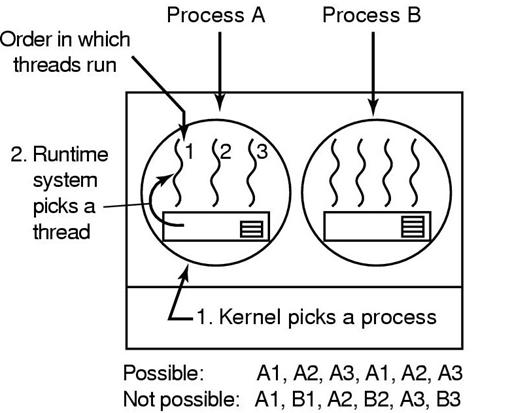
\includegraphics[scale = 0.3]{assets/ModernOperatingSystems_b0cb9.png}
	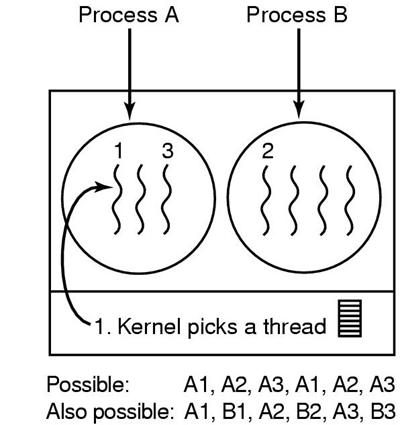
\includegraphics[scale = 0.3]{assets/ModernOperatingSystems_98c42.png}
	\caption{用户级线程调度 , 内核级线程调度  }
\end{figure}

\section{进程间通信,Inter Process Communication , IPC , 进程同步}

进程间通讯主要有3个问题:
\begin{itemize}
	\item 进程如何把信息传递给另一个进程
	\item 确保两个或更多的进程在关键活动中不会出现交叉。
	\item 与正确的顺序有关(如果该顺序是有关联的话)
\end{itemize}

进程间通讯的解决方案,同样适用于线程间通讯。

{\color{blue}Murphy 法则:任何可能出错的地方终将出错。}

\subsection{数据竞争}
多进程进程数据共享的时候,可能会出现数据竞争的问题。

其中一个解决办法是,建立临界区\footnote{\textbf{临界区:对共享内存进行访问的程序片段。}}
,对进程适当地安排,使得两个进程不可能同时处于临界区内。(即同一时间,只有一块代码(临界区)能操作临界资源)

对于一个好的解决方案,临界区需要满足一下4个条件:
\begin{itemize}
	\item 任何两个进程不能同时处于其临界区(互斥)
	\item 不应对CPU的速度和数量做任何假设
	\item 临界区外运行的进程不得阻塞其他进程(有闲让进)
	\item 不得使进程无限期等待进入临界区(有限等待)
\end{itemize}

\subsection{忙等待的互斥}
\textbf{忙}体现在,当一个进程想要进入临界区,先检查是否允许进入,若不允许,则该程序将原地等待,直到允许为止。

这种方法不仅浪费了CPU时间,而且可能引起优先级倒置等问题,但是如果切换上下文的时间开销大于忙等待的话,还是选择忙等待好。

忙等主要有以下6类:
\begin{itemize}
	\item 屏蔽中断\\
	      使每个进程在刚刚进入临界区后立即屏蔽所有中断,并在就要离开之前再打开中断。\\
	      屏蔽中断使系统底层的调用,不适合用户操控,而适合操作系统控制。\\
	      并且,对于多CPU的情况下,disable指令只对执行这个指令的CPU有效。
	\item 锁变量\\
	      就是不断循环判断,直到满足变量为某个值的条件。\\
	      这个方法判断的读取,和进入循环后的修改是分两步进行的,可能会被其他进程中断,进而导致冲突。
	\item 严格轮换法\\
	      每个进程轮流访问,当时不适合一个进程比另一个进程慢很多的情况。\\
	      尽管该算法避免了所有的竞争可能,但是它违背了临界区的条件3,所以不是一个好的方案
	\item Peterson解法
	      \begin{figure}[H]\centering
		      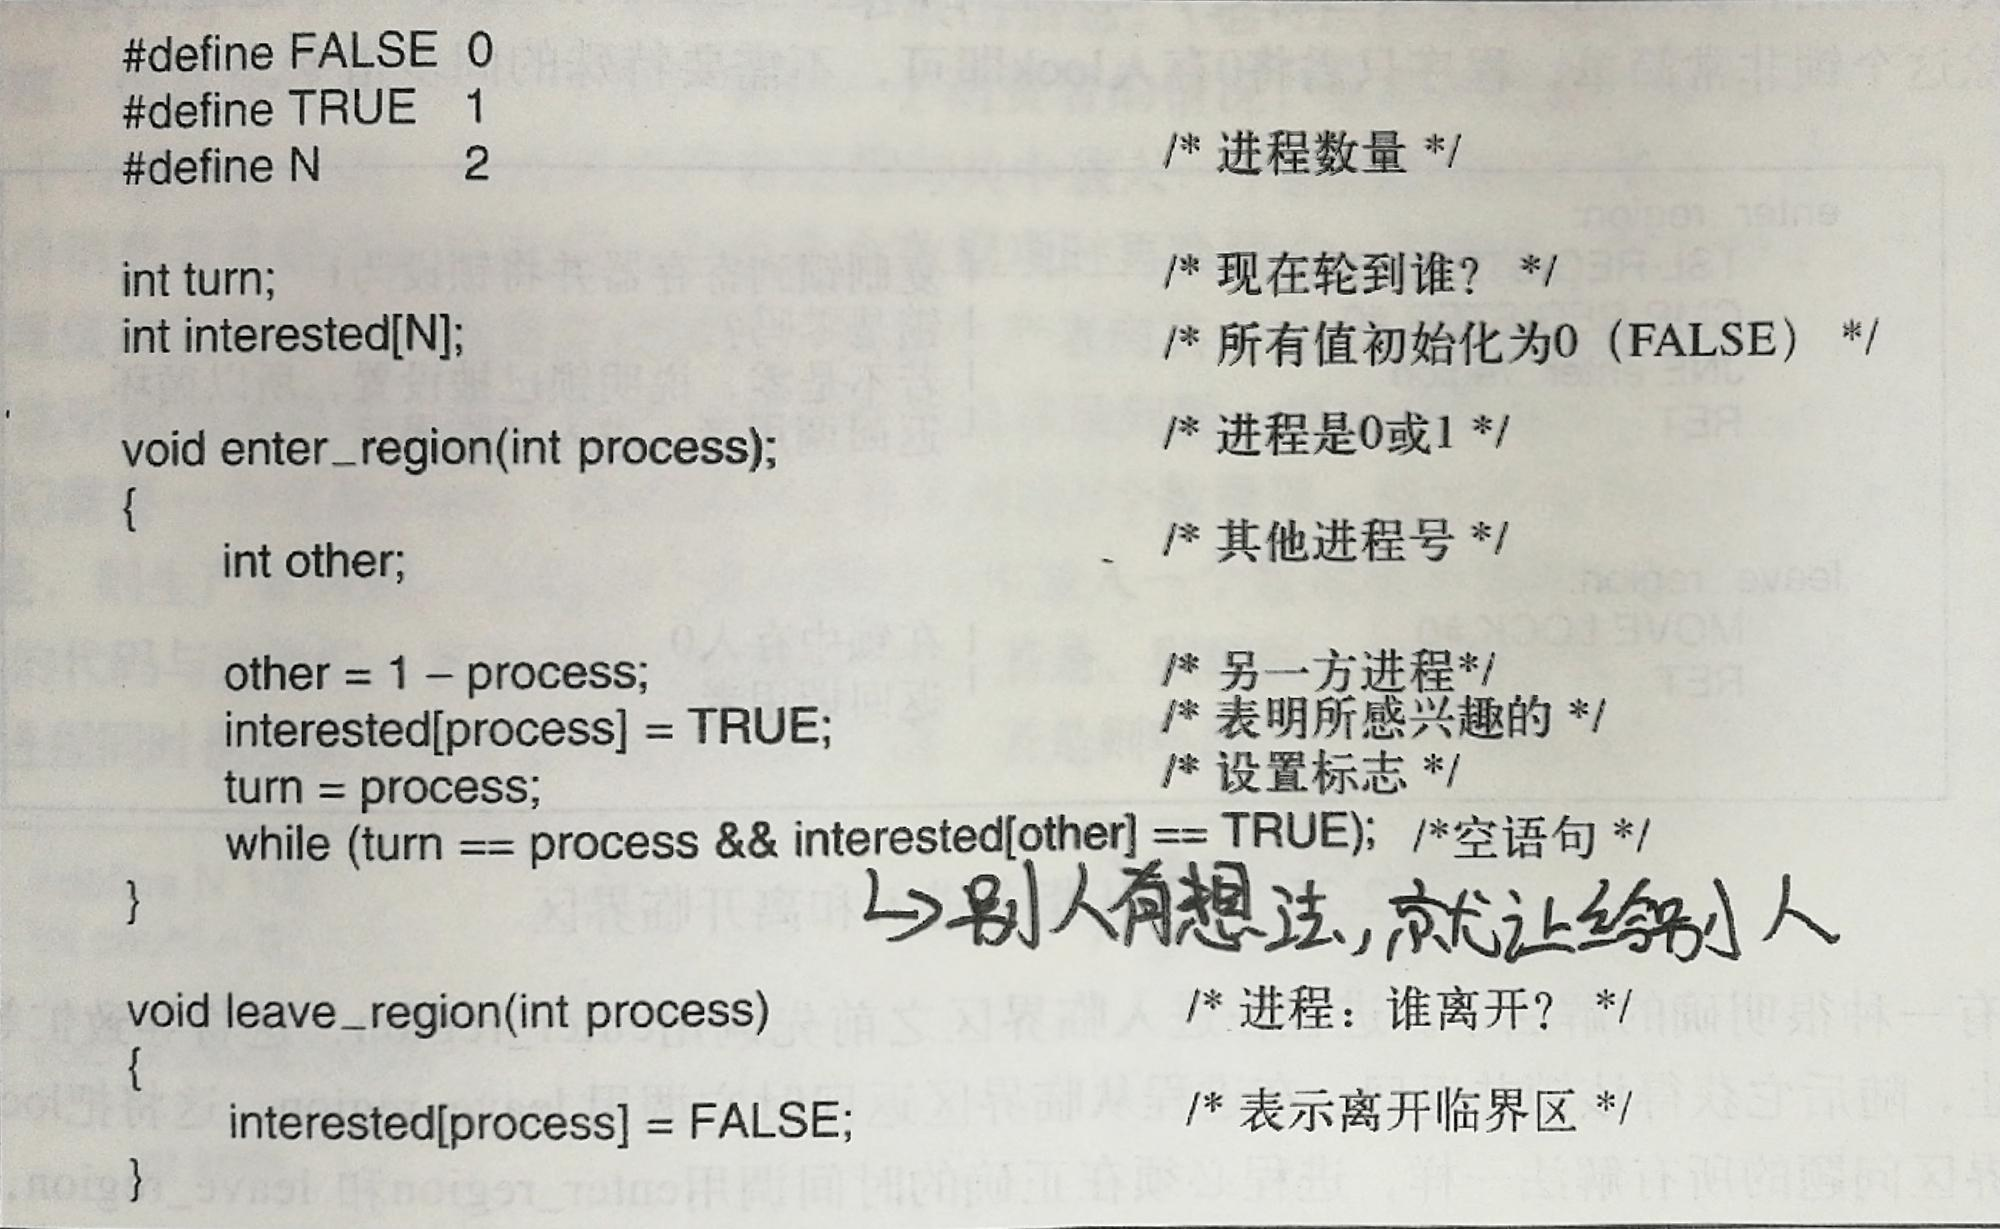
\includegraphics[scale = 0.2]{assets/ModernOperatingSystems_97ad7.png}
		      \caption{Peterson解法}
	      \end{figure}
	      增加了一个所谓的意愿变量,在进入临界区前,先考虑别人的意愿,如果其他人也有需求,则进入循环等待。\\
	      考虑两个进程几乎同时调用$enter\_region$的情况,\\
	      他们都将自己的进程号存入$trun$,但只有后保存进去的进程号才有效,前一个因被重写而丢失。\\
	      假设进程1是后进入的,那么进入到循环的时候,进程1 将循环等待,而进程0则成功进入临界区。\\
	      因此,不会出现死锁的情况。

	      {\color{blue}似乎只使用于双进程的情况?}
	\item TSL 指令(Test and Set Lock)\\
	      锁变量法出问题的原因,是测锁和加锁两步是分开执行而导致的冲突。\\
	      TSL则是一次执行这两个操作。\\
	      执行TSL指令的CPU将锁住内存总线,以禁止其他CPU在本指令结束之前访存。\\
	      一个可替代TSL指令是\textbf{XCHG},它原子性地交换两个位置的内容。
\end{itemize}

\subsection{睡眠唤醒}

忙等的缺点是会循环等待进入临界区,这浪费了CPU时间,一个可选的方案是使用 \textbf{睡眠}和\textbf{唤醒}的方法。

自动睡眠(阻塞):当无法进入临界区的时候程序进入阻塞状态。

被动唤醒:当一个进程退出临界区的时候,唤醒下一个访问临界区的进程

这个方法并不是很好,可能会出现一个进程想要睡眠却被另一个进程唤醒的情况。

\subsection{信号量 Semaphore}
信号量与变量的区别:信号量的操作都是原子性的。

一旦一个信号量操作开始,则在该操作完成或阻塞之前,其他进程均不得访问该信号量。

一个信号量有两个部分组成,一个是资源的数量,一个是等待资源的列表。

信号量主要有两个操作:
\begin{itemize}
	\item down\\
	      申请资源,同时资源数减一(down 1) ,如果减一之后资源数为0 ,则把这个进程加入到等待列表中
	\item up\\
	      释放资源,同时资源数加一(up 1) ,如果加一之后资源数还是小于等于0,则从等待资源的进程列表中取出一个进程唤醒
\end{itemize}

\subsection{互斥量 mutex}
互斥量是信号量的一个简化版本,它只有两个状态:解锁和加锁。

有以下几对指令形式,取其中一种表示即可:
\begin{itemize}
	\item down-up
	\item wait-signal\\
	      首先申请(等待)到资源才能继续
	\item lock-unlock\\
	      首先先加锁才能继续
\end{itemize}

\subsection{管程 Monitor}
在管程内,任意时刻只有一个活跃进程。\\
具体例子:java 的 synchronized关键字(被这个关键字标记的方法,同一时间只有一个能运行)
\begin{figure}[H]\centering
	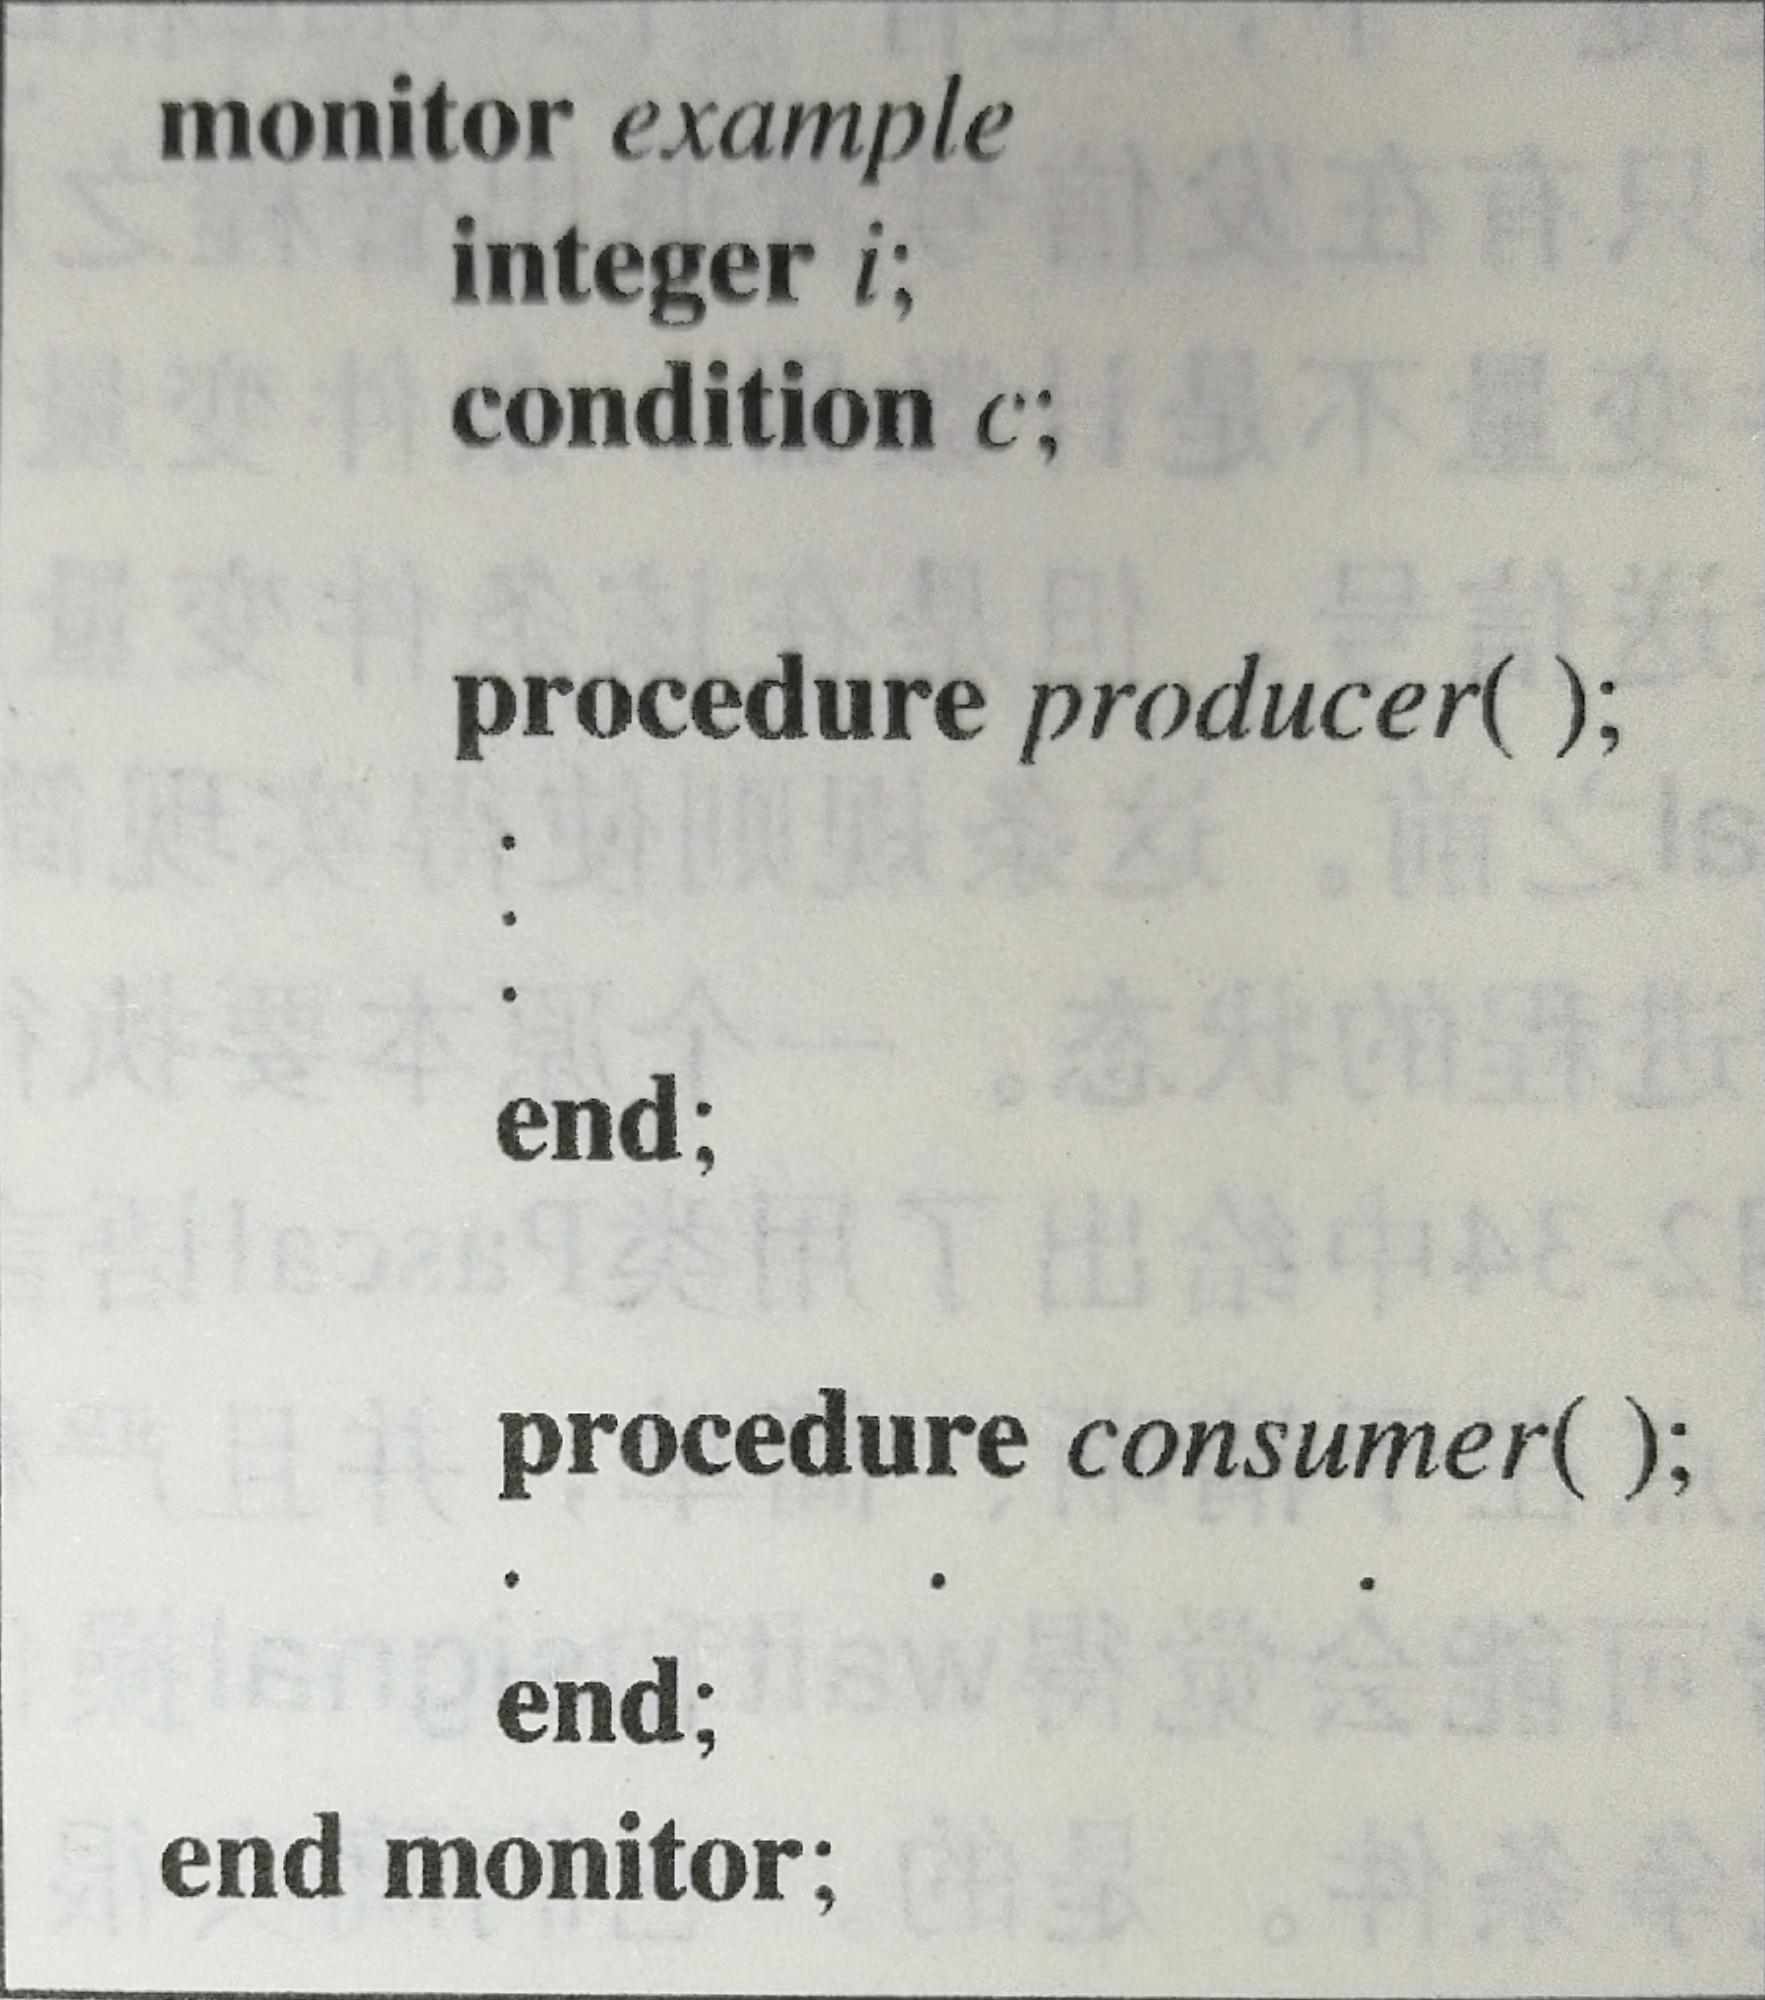
\includegraphics[scale = 0.1]{assets/ModernOperatingSystems_f64a5.png}
	\caption{管程}
\end{figure}
\begin{figure}[H]\centering
	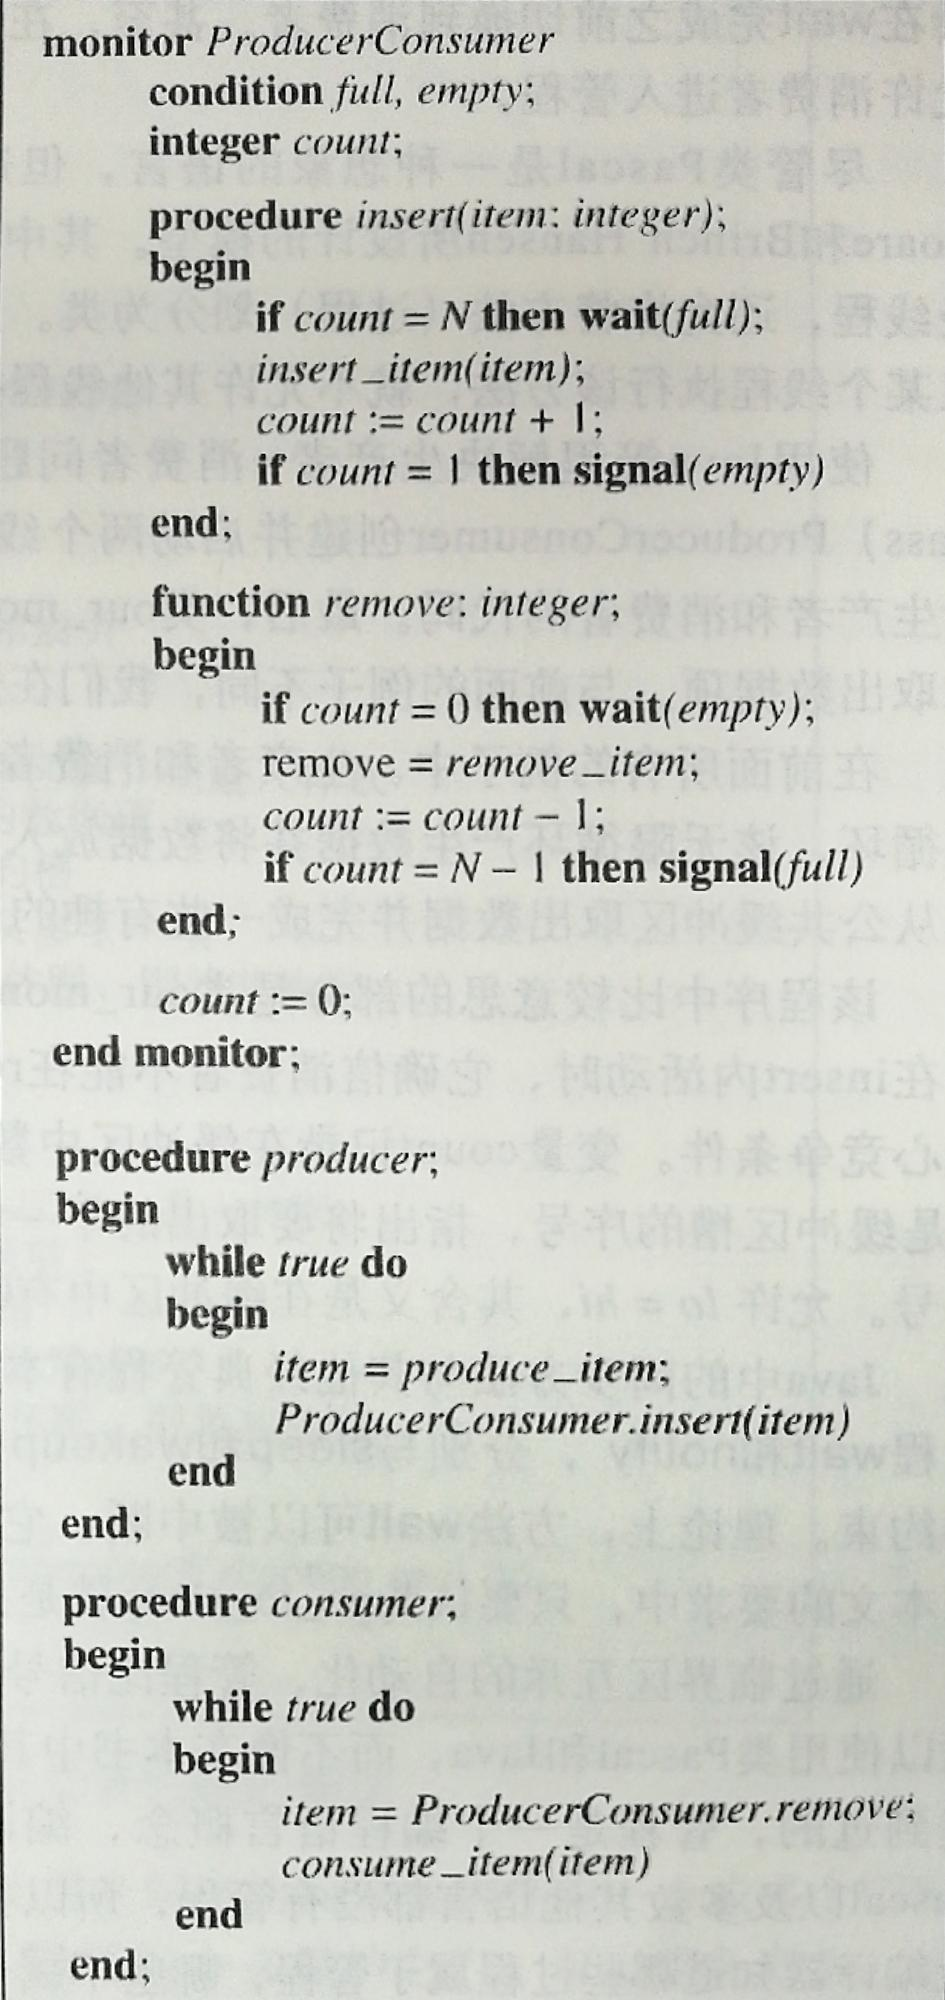
\includegraphics[scale = 0.3]{assets/ModernOperatingSystems_061b9.png}
	\caption{使用管程实现的生产者和消费者问题多的解法框架。}
\end{figure}

\subsection{消息传递}
使用消息传递(send/receive)进行通讯,这种进程通讯的方法是使用系统调用而不是语言成分。

主要有两大类:
\begin{itemize}
	\item 有缓冲
	\item 无缓冲\\
	      在发送之后,进入阻塞直到对方确认
\end{itemize}

\subsection{屏障}
屏障:进程组内所有进程就绪之后才进入下一个阶段。

% \subsubsection{5个经典的 ICP问题}
%
% \paragraph{生产者消费者问题}
%
% {\color{red}后面补上各种策略}
%
% \paragraph{环形缓冲区问题}
%
% {\color{red}没讲}
%
% \paragraph{读者写者问题}
% 多个读者可以同时读取,同时只有一个读者能写,并且不能同时读写。
% 问在怎么不死锁的情况下按规则进程读写?
%
% 解决方法:
% \begin{itemize}
%   \item 第一次读写的时候加锁,最后读写的时候解锁。
%   \item 在控制上面的加锁判断的时候,需要进行互斥操作(即要套上另一个锁再进行加锁解锁的判断和操作)
% \end{itemize}
%
% \paragraph{哲学家问题}
% 哲学家思考和吃面条。
%
% 解决办法:保证操作的原子性,一次必须同时取左右两边两个叉子,不能取则放弃

\section{死锁}
\subsection{死锁}
\textbf{资源}:可以分为共享资源和专有资源,可以分为抢占资源和不可抢占资源

资源分为可抢占资源和不可抢占资源两种:
\begin{itemize}
	\item 可抢占资源 : 可以从拥有它的进程中抢占而不会产生任何副作用,比如存储器
	\item 不可抢占资源 : 不在引起相关计算失败的情况下,无法把它从占有它的进程处抢占过来\\死锁和不可抢占资源有关
\end{itemize}

\textbf{死锁的定义:}  如果一个进程集合中的每个进程都在等待只能由该进程集合中的其他进程才能引发的事件,那么该进程集合就是死锁的

\textbf{产生死锁的4个条件:}
\begin{itemize}
	\item 互斥条件 : 每个资源要么已经分配给了一个进程,要么就是可用的
	\item 占有和等待条件 : 已经得到某个资源的进程可以再申请新的资源
	\item 不可抢占条件 : 已经分配给一个进程的资源不能强制性地被抢占,它只能被占有它的进程显式 释放\\和1类似, 但是两者是从不用对象的角度来描述的
	\item 环路等待 : 死锁发生时, 系统中一定有两个或两个以上的进程组成的一条环路,该环路中的每个进程都在等待着下一个进程所占有的资源
\end{itemize}

对于死锁有4种处理策略:
\begin{itemize}
	\item 忽略死锁,出事的时候重启 : 鸵鸟算法
	\item 检测死锁和恢复
	\item 动态分配资源来避免死锁
	\item 预防死锁 : 破坏死锁的4个必要条件之一
\end{itemize}

\subsection{死锁预防}
死锁预防:破坏产生死锁的4个基本条件之一

\textbf{破坏互斥条件:}采用假脱机\footnote{脱机:CPU不参与}的策略,使用可共享的设备来模拟不可共享的设备\\
如:打印机采用打印机队列来处理

\textbf{破坏占有和不可等待条件:}一次申请所有的资源\\
但是往往需要的资源是不可知道的,并且一次申请资源的策略对于资源的利用率低\\
若是知道所需要的资源,往往采用银行家算法以提高资源的利用率

\textbf{破坏不可抢占条件:}采用虚拟的设备,使得不可抢占资源变得可以抢占,比如多个进程同时往声卡输出,实际上对于进程来说,它操作的声卡是虚拟的

采用虚拟设备的方法(假脱机)能同时破坏互斥和不可抢占两个条件

\textbf{破坏环路等待条件} : 对资源进行编号 , 进程在任何时刻都可以提出资源申请,但是所有申请必须按照资源编号的顺序(升序)提出

\begin{figure}[H]
	\centering
	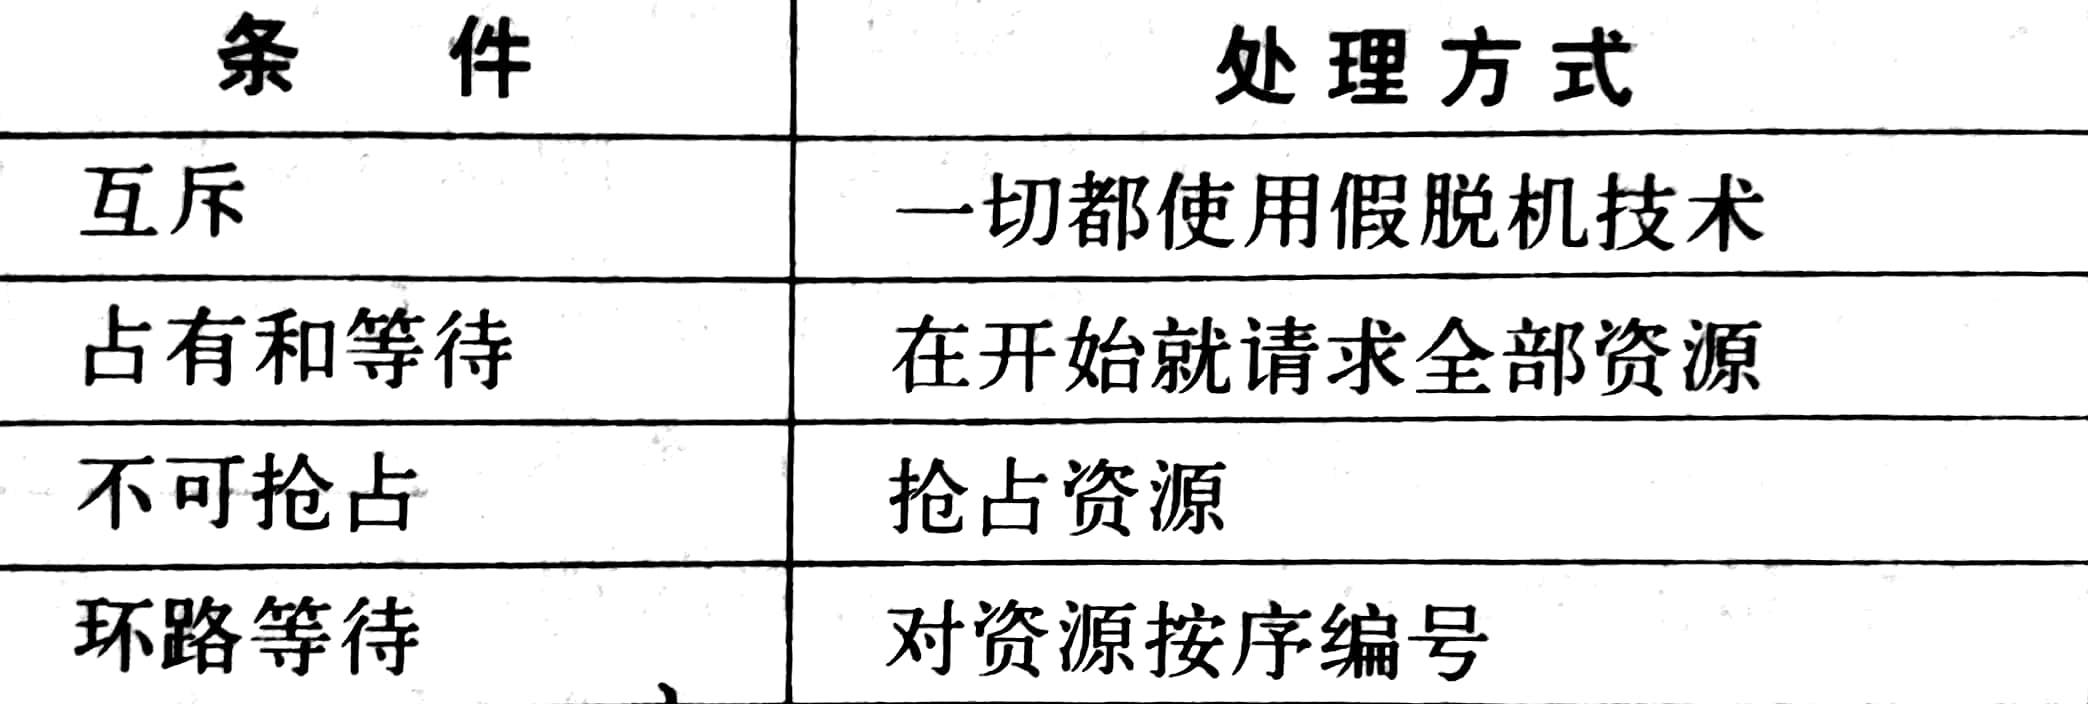
\includegraphics[scale = 0.1]{assets/ModernOperatingSystems_d2112.png}
	\caption{预防死锁方法汇总}
\end{figure}

\subsection{死锁避免}
和死锁预防概念类似,但是不同,死锁避免是可能产生死锁,但是选择合理得方式来避免死锁,而死锁预防,则是杜绝死锁产生的条件

可视化的角度理解:资源轨迹图:CPU分配的时候,要避开阴影区域

可视化的角度和算法不太一样,

\textbf{安全状态和不安全状态:}若是把资源都非给某个进程,最终能使得所有进程都能结束,则是安全状态

资源分配主要采用银行家算法

\begin{itemize}
	\item 当一个一个资源请求来的时候,先判断接受这个请求之后的状态是否是安全状态
	\item 判断一个状态是否是安全状态,则是把剩下的所有资源都分配给某个进程,等待进程完成,再回收资源,再分配,循环直到所有进程都结束,若是不能结束,则不安全
	\item 单个进程怎么会有死锁?资源的数目不够进而产生死锁
	\item 银行家算法不是一次申请所有资源,而是需要的时候再申请,若是一次请求是不安全的,则延后该请求,先完成其他进程的请求,直到这个请求是安全的
\end{itemize}

\subsection{死锁的检测与恢复}
死锁检测有两个算法
\begin{itemize}
	\item $O(n^2)$,从每个节点出发看是否能走到已经走过的节点(dfs),是则有回路
	\item 多资源死锁检测
\end{itemize}

从死锁中恢复:
\begin{itemize}
	\item 抢占资源 : 临时将某个资源从它当前的所有者那里转移到另一个进程
	\item 利用回滚\\
	      出错,存档,避开错误\\
	      回滚不需要回滚全部进程,只需要回滚某些,或某个进程即可
	\item 杀死某些死锁的进程\\
	      这个和回档类似,这个相当于直接回滚到了起点
\end{itemize}

\subsection{两端加锁协议}
和回滚类似,申请资源先上锁,用完之后才解锁\\
数据库专用,对于申请的资源已经加锁的情况,则释放自己已经加的锁,再重新申请资源

\subsection{通信死锁}
通信也可能产生死锁,比如A发送消息给B,B等待接受消息,A等待B的确认消息,若是A发送的包丢失,则两者都需要等待\\
这种情况一般采用某种协议来进行信息正确性的保证,比如超时重发什么的

\subsection{活锁}
活锁,和死锁的现象类似,但是活锁的进程不是进入阻塞态,而是忙等,

{\color{red}这个和数据库了解到的活锁不太一样呢,数据库那个情况 在这里叫 饥饿}

\subsection{饥饿}
未被阻塞,但是被无限地退后,导致进程毫无进展

\section{存储管理}
\textbf{内存管理:}
\begin{itemize}
	\item [1.] 监控和管理已用和空闲的内存
	\item [2.] 分配内存
	\item [3.] 回收内存
	\item [4.] 保护\\
	      保护已占用的内存不被影响
	\item [5.] 虚拟化\\
	      内存若不够使用则使用虚拟化技术
\end{itemize}

\spaceline
\textbf{内存管理需要考虑的因素:}
\begin{itemize}
	\item 有限的存储空间
	\item 尽可能高效地运行
	\item 有足够大的低速存储
\end{itemize}

\spaceline
\textbf{分层存储的好处:}
\begin{itemize}
	\item 缓解高速缓存和低速存储之间速度不一致的问题
	\item 缓解高速缓存和低速存储空间容量不一致问题
\end{itemize}

\textbf{3种存储方式:}
\begin{itemize}
	\item 无存储抽象:每个程序直接访问物理内存,引用绝对的物理内存
	\item 有存储抽象 : 地址空间
	\item 虚拟内存
\end{itemize}

\subsection{无存储抽象:}

\spaceline
\textbf{无存储抽象:}程序引用绝对的物理地址

多道程序运行的2种方案
在此方式是可以通过 \textbf{把内存写入磁盘} 或 \textbf{静态重定位} 来实现多道程序运行 \\
静态重定位是指 ,程序内编码相对地址 , 通过静态的偏移常量来重定位物理地址 ,使得多个程序的绝对物理地址不相交

\spaceline\textbf{静态重定位:}
采用绝对的物理地址不好,那么可以采用逻辑地址(静态重定位技术)\\
静态重定位技术,链接的时候地址修正成正确的物理地址(代码上是逻辑地址,链接之后是绝对的物理地址,因此是静态)\\
但是,使用静态重定位技术需要解决 代码中数字和地址的区分问题

\subsection{存储抽象 : 地址空间}
\textbf{内存抽象:}每个进程建立一个地址空间

\textbf{地址空间} : 是一个进程可用于寻址内存的一套地址集合.每个进程都有一个自己的地址空间,并且该空间独立于其他进程(除了在特殊情况下进程需要共享它们的地址空间外)

\textbf{逻辑地址:}逻辑空间中的地址\\
\textbf{物理地址:}物理空间中的地址

\spaceline\textbf{寻址方案:}
\textbf{动态重定位} : 把每个进程的地址空间映射到物理内存的不同部分(通过 \textbf{基址寄存器}  和\textbf{界限寄存器} 实现)

使用这两个寄存器时, 程序装载到内存中连续的空闲位置 且装载期间无须重定位

当一个进程运行时 , 程序的起始物理地址装载到基址寄存器, 程序的长度装载到界限寄存器中

上述的做法会存在地址越界的问题

\subsection{交换技术}
当出现出里内存超载时,有两个通用的解决办法 :
\textbf{交换技术} 、 \textbf{虚拟内存}

\textbf{交换技术} : 把一个进程 \textbf{完整} 调入内存 , 使该进程运行一段时间 ,然后把它 \textbf{存回} 磁盘

内存交换可能出现的问题:
\begin{itemize}
	\item 重定位问题 :
	      它换入的时候通过软件 或者 (大部分情况) 在程序运行期间通过硬件对其地址进行重定位
	\item 内存空洞 : 使用内存紧缩技术 , 但是一般不进行这个操作因为很耗时
\end{itemize}

\textbf{内存紧缩} : 交换在内存中产生了多个空闲区(空洞) , 通过把所有进程尽可能向下移动,有可能把这些小的空闲区合并成一大块

数据段可以增长,数据增长之后内存怎么分配?
\begin{itemize}
	\item 若周围(上和下)有空闲区, 则直接把该空闲区分配给该进程,在这个空闲区中增大
	\item 若相邻的是进程 , 则把需要增大的进程移动到足够大的区域
	\item 若程序在内存中不能增长, 且磁盘上的交换区也满了, 则挂起这个进程 ,直到有空闲区(或直接结束进程)
	\item 当换入或移动的时候,可以余下分配一些额外的内存 \\
	      为了减少交换的频率,在程序创建的时候,可以预留与部分空间用来未来程序的增长,当预留的不够了,再进行上面的操作
	\item 一个优化的做法 : 采用两段增长的方式,堆+栈
\end{itemize}

\subsubsection{空闲内存管理}
\textbf{空闲空间管理:}有两种策略
\begin{itemize}
	\item 位图管理
	\item 链表
\end{itemize}

\paragraph{位图管理}
\textbf{位图管理:}把内存按一定大小划分,每个区域使用一位进行表示是否空闲
\begin{itemize}
	\item 划分单元小,则位图大,空间利用率与时间效率相矛盾
	\item 查找空间是低效的,因为查找连续的0是一个耗时的操作
\end{itemize}

\paragraph{链表管理}
\textbf{链表:}使用链表管理,链表的节点是一个进程,或者是两个进程之间的空闲区域
\begin{itemize}
	\item 链表按地址排序,则出现新的空闲空间的时候,可较快地合并相邻的元素
	\item 使用双向链表 : 更易于找上一个节点,并检查是否可以合并
\end{itemize}

\textbf{空闲空间的分配方式}
\begin{itemize}
	\item 首次适配 : 沿着链表找 ,找到足够大的空闲区 , 一部分划分给进程 , 剩下部分形成新的空闲区

	\item 下次分配 : 每次找到合适的空闲区就记录当前位置 ,下次在这个位置继续查找 , 使得物理内存得到均衡使用
	\item 最佳分配 : 搜索整个链表 ,找出一个能容纳进程的最小空间
	\item 最差分配 : 最佳适配会产生很多非常小的空闲区 , 为了避免这个问题 , 分配最大的空闲区
\end{itemize}

\textbf{一个优化}  :链表划分成两个链表,一个链表放进程,一个链表放空闲内存,这样上述的4个算法都能提速

对空闲区块链表排序 ,可以提高最佳分配算法的速度 , 首次适配算法和最佳适配算法一样快, 而下次分配算法没有意义

\textbf{快速分配算法}:为常用大小的空闲区单独维护链表 ,有一个n项的表 ,该表第一项为大小为4KB的空闲区链表表头的指正 , 第二项为8KB, 以此类推

快速分配算法和空闲块排序的策略都存在 寻找相邻块进行合并的 代价十分大的缺点

\subsection{虚拟内存}
虚拟内存使程序在只有一部分被调入内存的情况下运行 , 由系统完成实际的覆盖块的换入和换出,这些工作全部交给计算机完成,而不用程序员实现

\textbf{基本思想:}
\begin{itemize}
	\item 每个进程都有各自的地址空间 , 把这个空间划分成多块 , 每块称为一个页面 , 每页有连续的地址范围
	\item 这些页被映射到物理内存 , 但不是所有的页都在内存中才能运行程序。
	\item 当程序一弄到一部分在物理内存中的地址空间时, 由硬件执行必要的映射
	\item 当程序引用到不在物理内存的地址空间时, 由操作系统负责将缺失的部分装入物理内存并重新执行失败的指令
\end{itemize}

\subsubsection{分页}
每个进程都有各自的地址空间 , 把这个空间划分成多块 , 每块称为一个页面 , 每页有连续的地址范围 , 这些页被映射到物理内存 , 但不是所有的页都在内存中才能运行程序。

对于物理内存 , 也划分成与页面等大的页框 , 用于存放页面

在使用虚拟内存的情况下 , 虚拟地址不是被直接送到内存总线上 , 而是被送到内存管理单元 (Memory Management Unit ,MMU)把虚拟地址映射为物理内存地址

RAM和磁盘之间的交换总是以整个页面为单元进行的

\textbf{页表:}(每个进程)存放虚拟页号与物理页框号的映射关系 , 虚拟地址呗分为 \textbf{虚拟页号(高位部分)} 和 \textbf{偏移量(低位部分)}两部分

虚拟页号可以作为页表的索引

\textbf{虚拟地址与物理地址的转换:}把虚拟地址的页号替换成所在的页框号即可

\textbf{页表项的结构}
\begin{figure}[H]
	\centering
	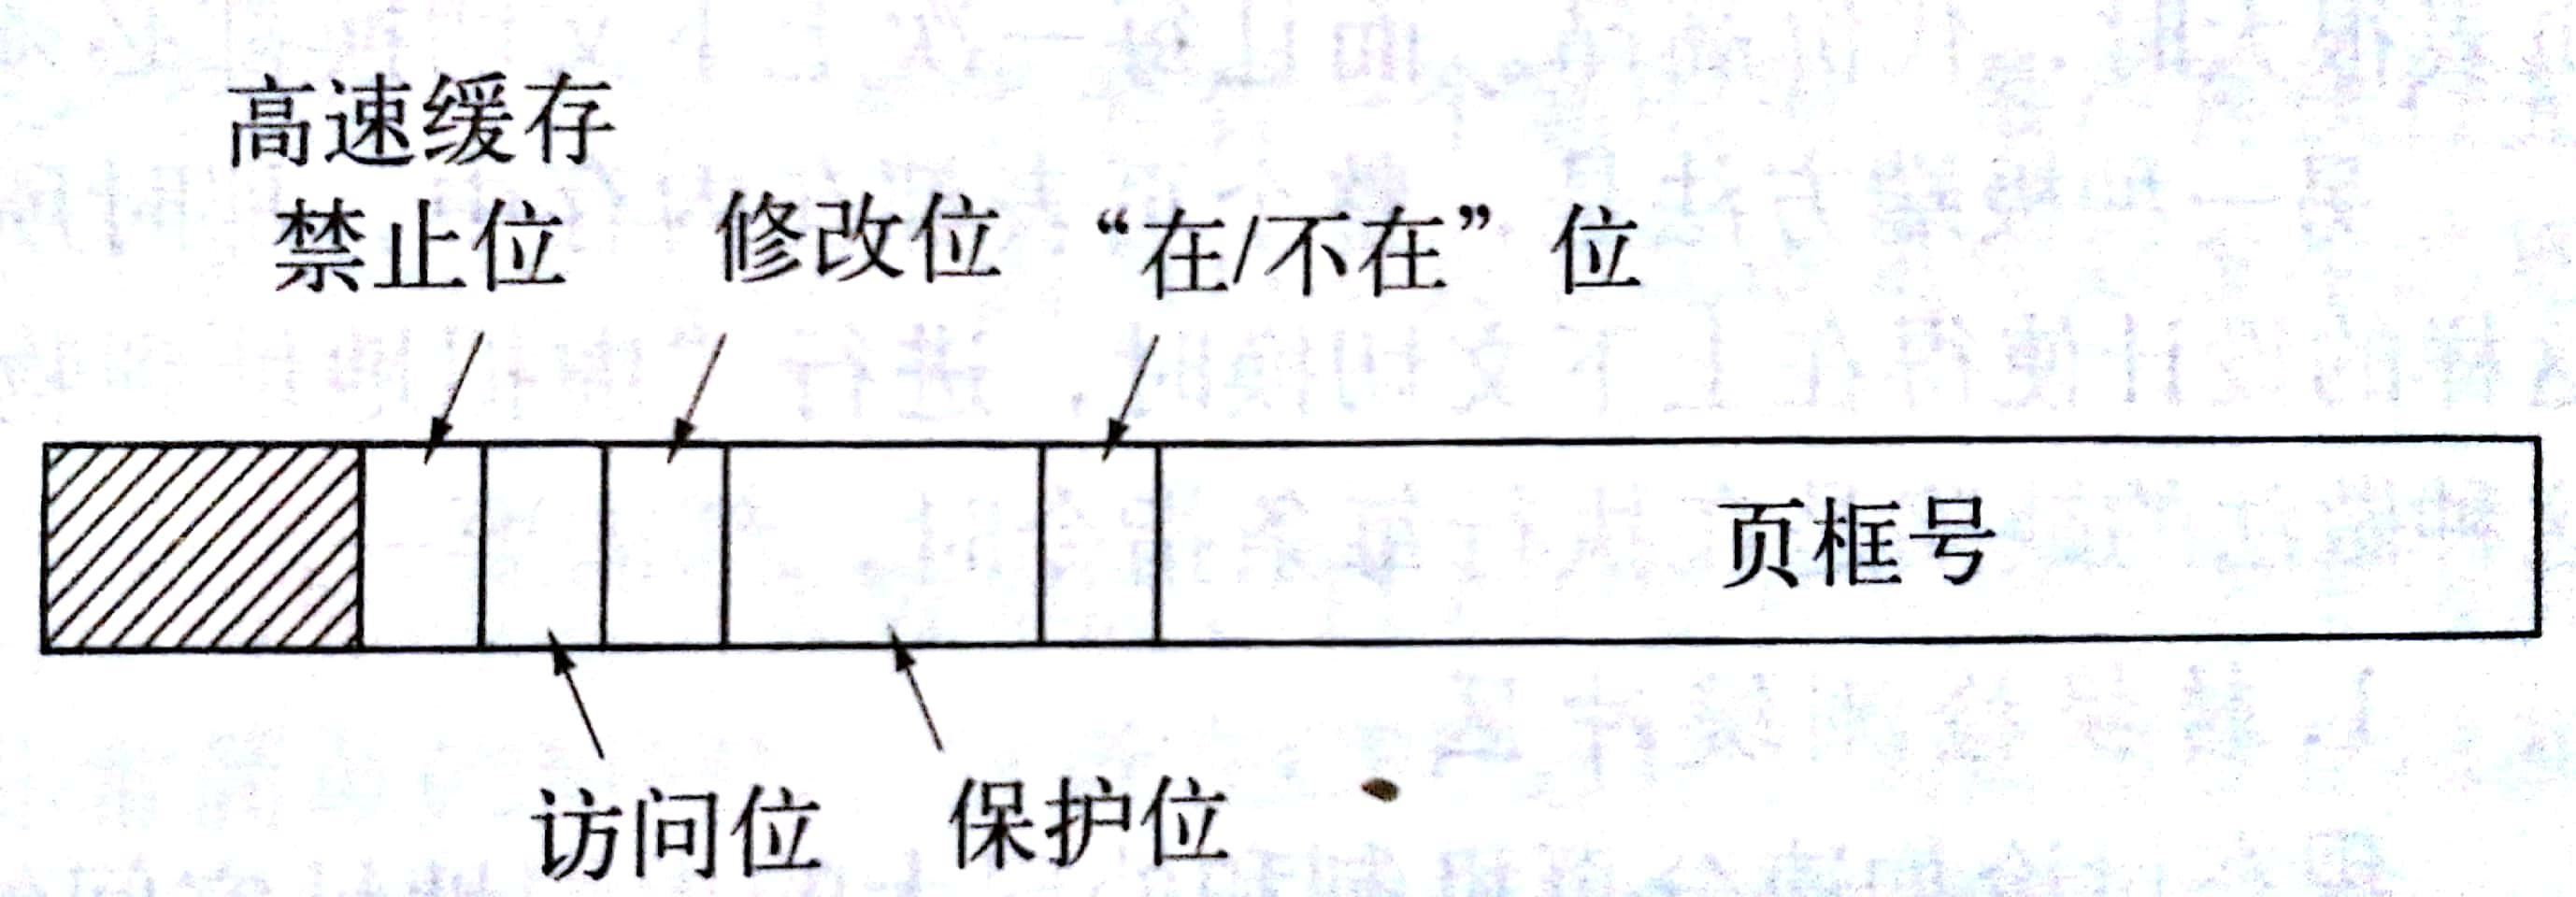
\includegraphics[scale = 0.1]{assets/ModernOperatingSystems_c9507.png}
	\caption{一个典型的页表项}
\end{figure}
上图是一个典型的页表项
\begin{itemize}
	\item 页框号 : 该页所在的物理页框编号
	\item 在/不在位 : 为1表示该表项有用, 为0引起缺页中断
	\item 保护位 : 指出一个页允许什么类型的访问
	\item 修改位 : 页面被修改过, 替换的时候必须把它写回磁盘
	\item 访问位 : 是否被访问过(用于页面淘汰算法)
	\item 高速缓存禁止位 : 禁止该页被高速缓存
\end{itemize}

\subsubsection{TLB}

\textbf{加速分页过程}:
一个加速方法:TLB,建立一个更高速的小表

对于大多出程序总是对少量的页面进行多次访问, 而不是相反, 因此,只有很少的页表项会被反复读取 ,而其他的页表项很少被访问

因此 , 为计算机设置一个小型的硬件设备,将虚拟地址直接映射到物理地址,而不必在访问页表 , 这种设备称为 \textbf{转换检测缓冲区 , Translation Lookaside Buffer , TLB}

\textbf{TLB工作过程}:
将一个虚拟地址放入MMU中进行转换时 , 硬件首先通过将该虚拟页号与TLB中所有表项同时(并行)匹配,判断虚拟页面是否在其中;

如果发现了一个有效的匹配 并且要进行的访问操作并不违反保护位 , 则将页框号直接从TLB取出而不必再访问页表

如果虚拟页面号确实是在TLB中 , 但指令试图在一个读页面上进行写操作 ,则会产生一个保护错误 , 就像对页表进行非法访问一样

如果不在TLB中 , 那么就进行正常的页表访问, 并从TLB中淘汰一个表项 , 用新找到的页表项替代它

\textbf{软件TLB管理}
当页面不在TLB中的时候(TLB访问失效),不再是由MMU到页表中查找并取出需要的页表项, 而是生成一个 \textbf{TLB失效} 并将 问题 \textbf{交给系统解决}

% 硬件TLB管理和软件TLB管理的区别:当一个页面访问在内存中而不在TLB中,将产生 \textbf{软失效}  ,那么此时要做的就是更新一下TLB , 不需要产生磁盘 I/O

\subsubsection{针对大内存的页表}
怎么处理巨大的虚拟地址空间 ?

\begin{itemize}
	\item 多级页表 : 避免把全部页表一直保存在内存中;
	\item 倒排页表 : 在实际内存中每个页框有一个表项 , 而不是每个虚拟页面有一个表项 \\
	      倒排页表 节省了大量空间 , 但是 虚拟地址到物理地址的转换会变得困难 , 它必须搜索整个倒排页表来查找某个表项\\
	      使用TLB解决查找问题 , TLB记录所有频繁使用的页面 , 地址转化就可以像通常页表一样快速 , 但是当TLB失效时 , 需要用软件搜索整个倒排页表:
	      \begin{itemize}
		      \item 建立一张散列表 , 虚拟地址来散列,
		      \item 当前所有的内存中具有相同散列值的虚拟页面被链接在一起
		      \item 如果散列表中的槽数与机器中物理页面数一样多,那么散列表的冲突链的平均长度将会是1 , 这将大大提高映射速度
	      \end{itemize}

\end{itemize}

\subsubsection{页面置换算法}
当发生缺页中断时, 操作系统必须在内存中选择一个页面将其换出内存 , 以便为即将调入的页面腾出空间

如果换出的页面在内存驻留期间已经被修改过, 就必须把它写回磁盘以更新该页面在磁盘上的副本,

如果该页面没有被修改过,那么它在此本的副本已经是最新的, 不需要回写 , 直接用调入的页面替换掉被淘汰的页面就可以了

\textbf{页面替换算法}
\begin{itemize}
	\item 最优页面置换算法 : 理想算法 , 每个页面使用该页面第一次被访问所要执行的指令数作为标记 ,替换标记最大的页面
	\item 最近未使用页面置换算法 NRU Not Recently Used
	      \begin{itemize}
		      \item 设置 RW 位 , 初始为 00
		      \item 每次访问写R, 每次写入 写W
		      \item 定期置R为0,以区别最近没有被访问的页面和被访问的页面
		      \item 优先淘汰低编号的页面(01表示没有被访问, 已被修改 , 这是因为R是被定期置0了)
	      \end{itemize}
	      算法隐含的意思 : 在最近一个时钟滴答中 , 淘汰一个没有被访问的已修改页面比淘汰一个呗频繁使用的干净页面好\\
	      虽然NRU的性能不是最好,但是已经够用了
	\item 先进先出置换算法 FIFO:适用于 商品撤销等场景
	\item 第二次机会页面置换算法(链表实现队列) :  FIFO , 但第一次出队列的时候,会重新加入队列\\
	      设置R位,初始为1 , 如果R位是0表示既老又未被使用,那么直接替换掉 , 否则把R位置为0 ,重新加入队列尾
	\item 时钟页面置换算法 : 效果和第二次机会页面置换算法一样 \\
	      但后者是链表实现 , 时钟算法是实现方式的优化  , 把所有页面都保存在一个类似钟面的环形链表中 , 一个表针指向最老的页面 \\
	      当发生缺页中断 , 就检查指针指向的页面的R位, 是1则置0 , 并移动指针,是0则替换
	\item 最近最少使用页面置换算法 LRU Least Recently Used:置换未使用时间最长的页面\\
	      已经很久没有使用的页面, 可能在未来很长一段时间仍然不会使用\\
	      硬件实现 1: 记录上一次被访问的时间
	      \begin{itemize}
		      \item 有一个64位的计数器C , 每个表项有一个列保存C的值
		      \item 每执行一条指令, 计数器+1
		      \item 每次访问内存后, 将当期C值保存到该页面的页表项中
		      \item 替换页表项保存的C值最小的页面
	      \end{itemize}
	      硬件实现 2 :
	      \begin{itemize}
		      \item 对于n个页框的机器, 维持一个初始值为0的$n\times n$的矩阵
		      \item 当访问第k个页框时 , 把第k行置为1 , 第k列置为0(第k行第k列最终为0)
		      \item 每行二进制值最小的就是 最近最少使用
		      \item 第二小的行就是下一个最近最少使用的
	      \end{itemize}
	      \begin{figure}[H]
		      \centering
		      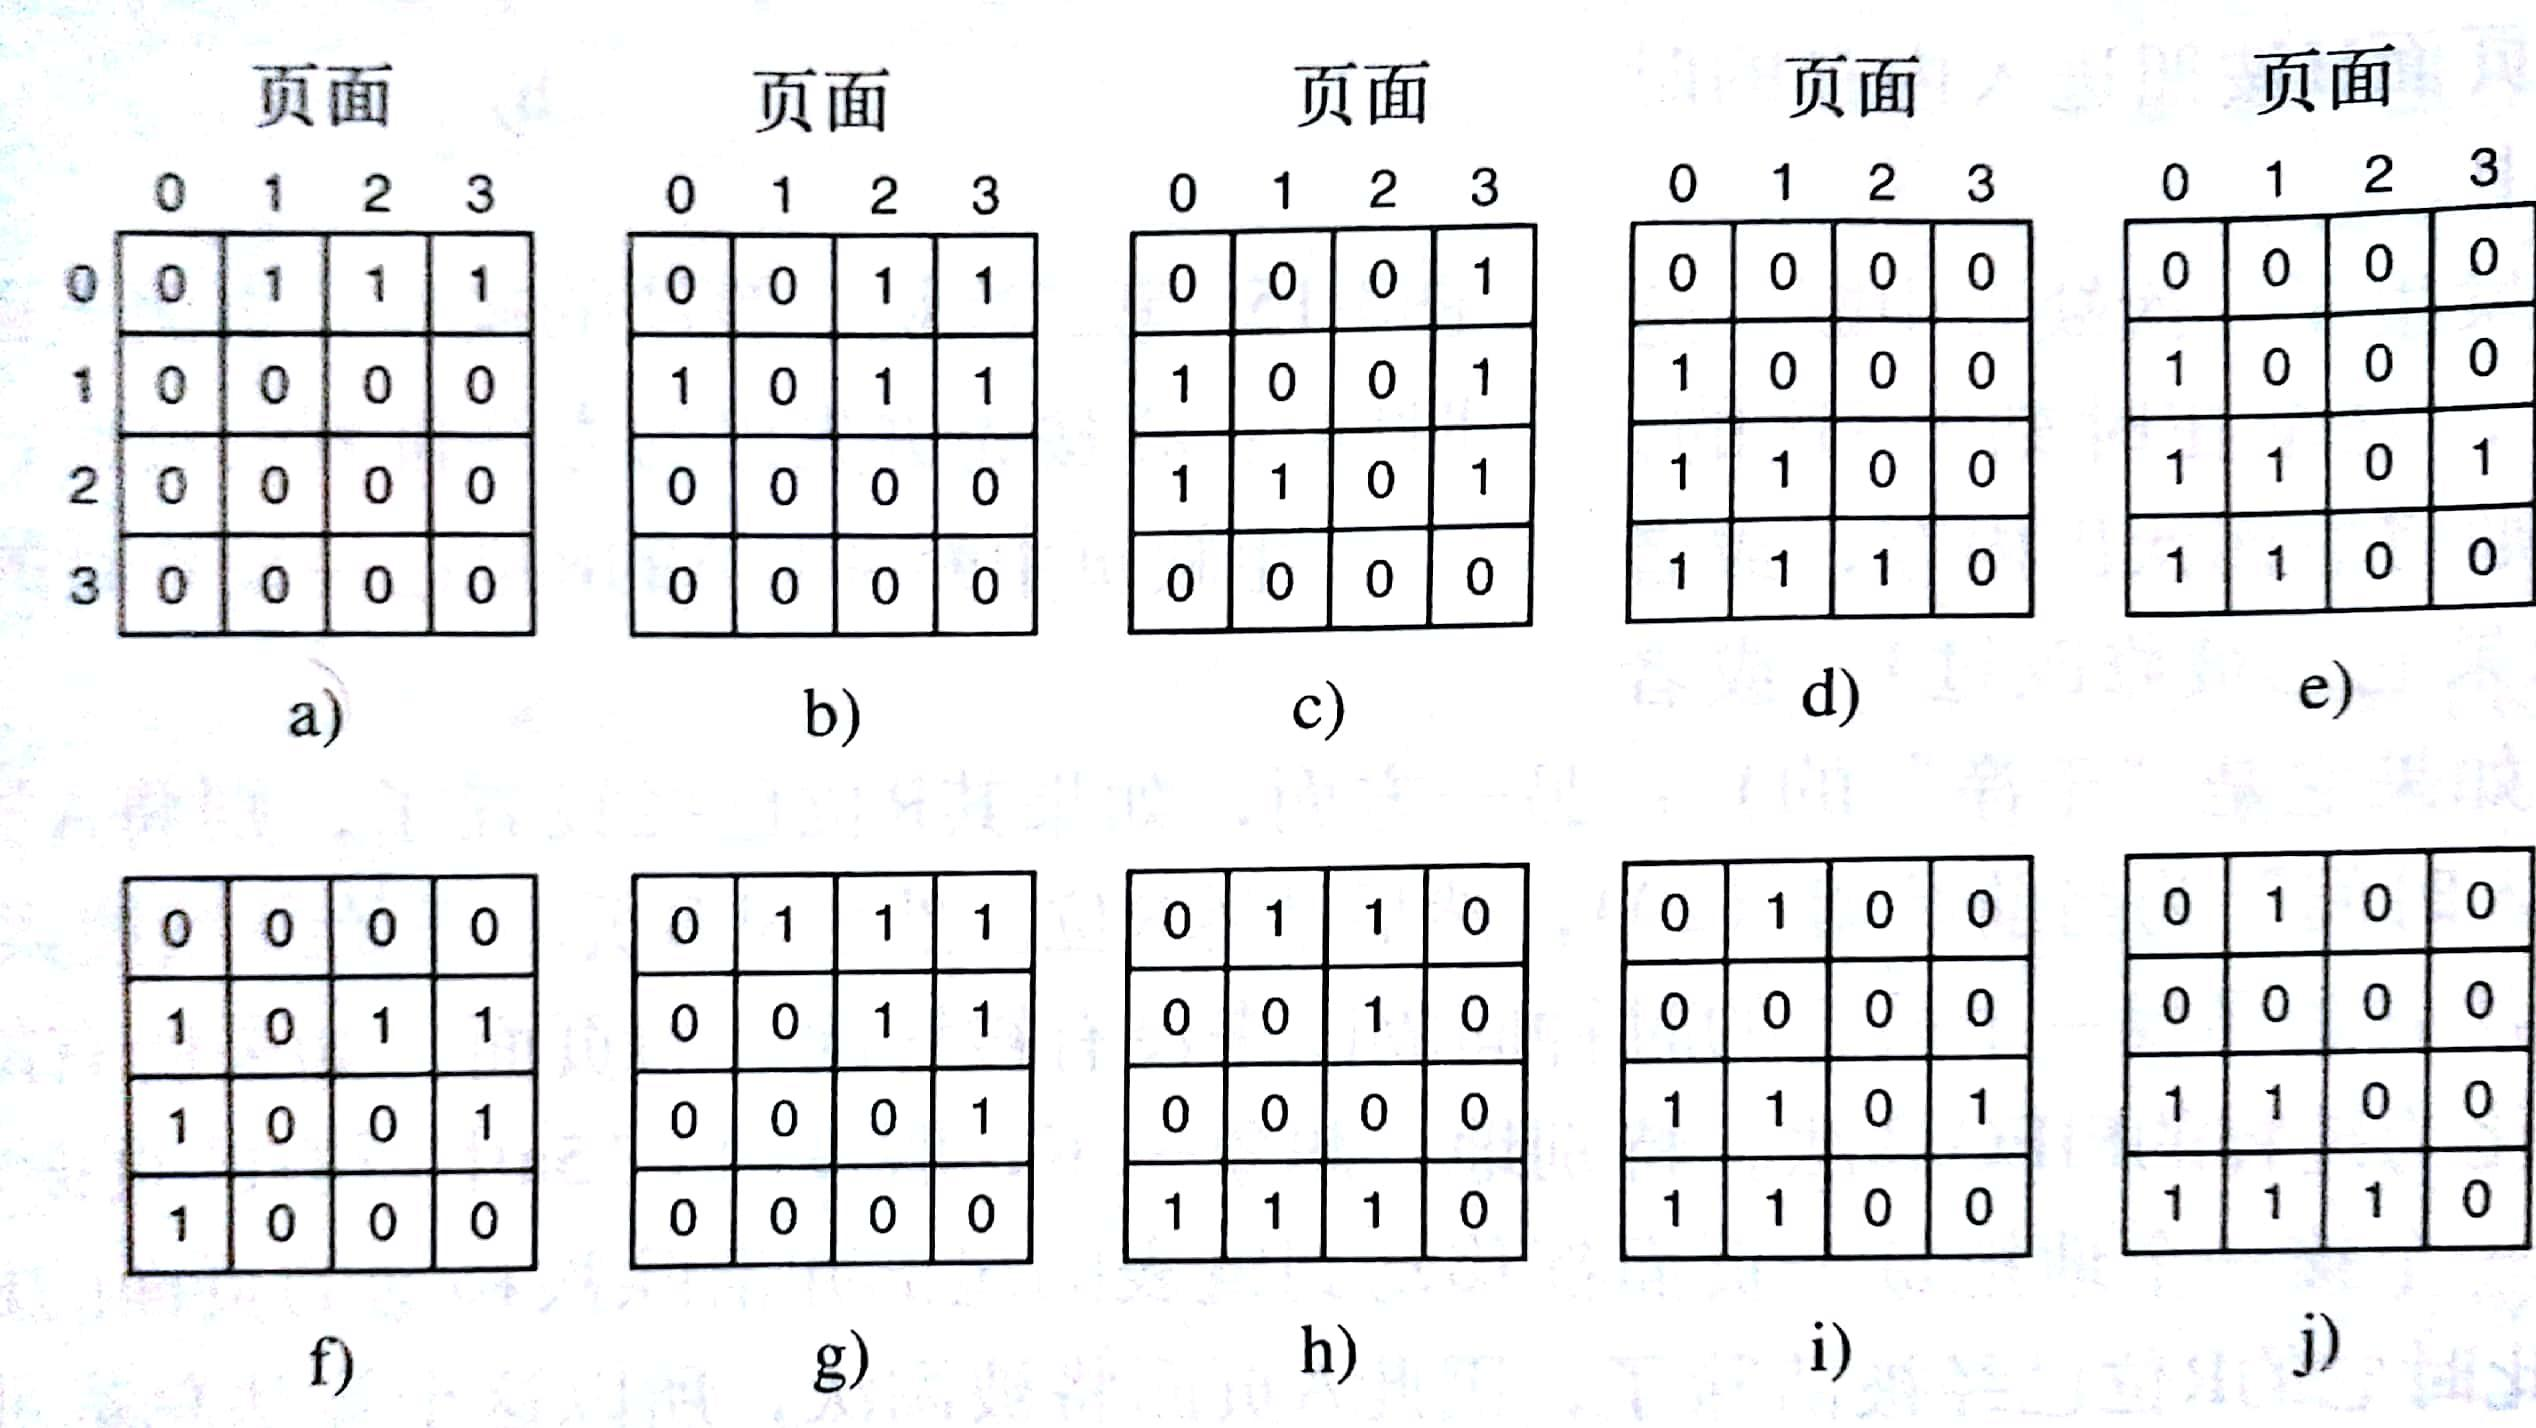
\includegraphics[scale = 0.1]{assets/ModernOperatingSystems_67c6f.png}
		      \caption{使用矩阵的LRU , 页面以0,1,2,3,2,1,0,3,2,3次序访问}
	      \end{figure}
	      但是很少计算机拥有这两种硬件
	\item 最不常用算法 NFU Not Frequently Used , LRU 软件模拟\\
	      将每个页面与一个软件计数器相关联,计数器初始为0,每次时钟中断时,由
	      操作系统臊面内存中的所有页面 , 将每个页面的R位(它的值为0or1)加到它的计数器 \\
	      置换计数器值最小的页面 \\
	      但是历史访问最多次 并不代表接下来要频繁访问
	\item 老化算法 Aging \\
	      对NFU进行修改 , 在R位被加之前,先将计数器右移动一位;\\
	      其次,将R位见到计数器最左端而不是最右端(因为右移,最高位一定为0 , 因此不存在最高位进位的情况)
	      \begin{figure}[H]
		      \centering
		      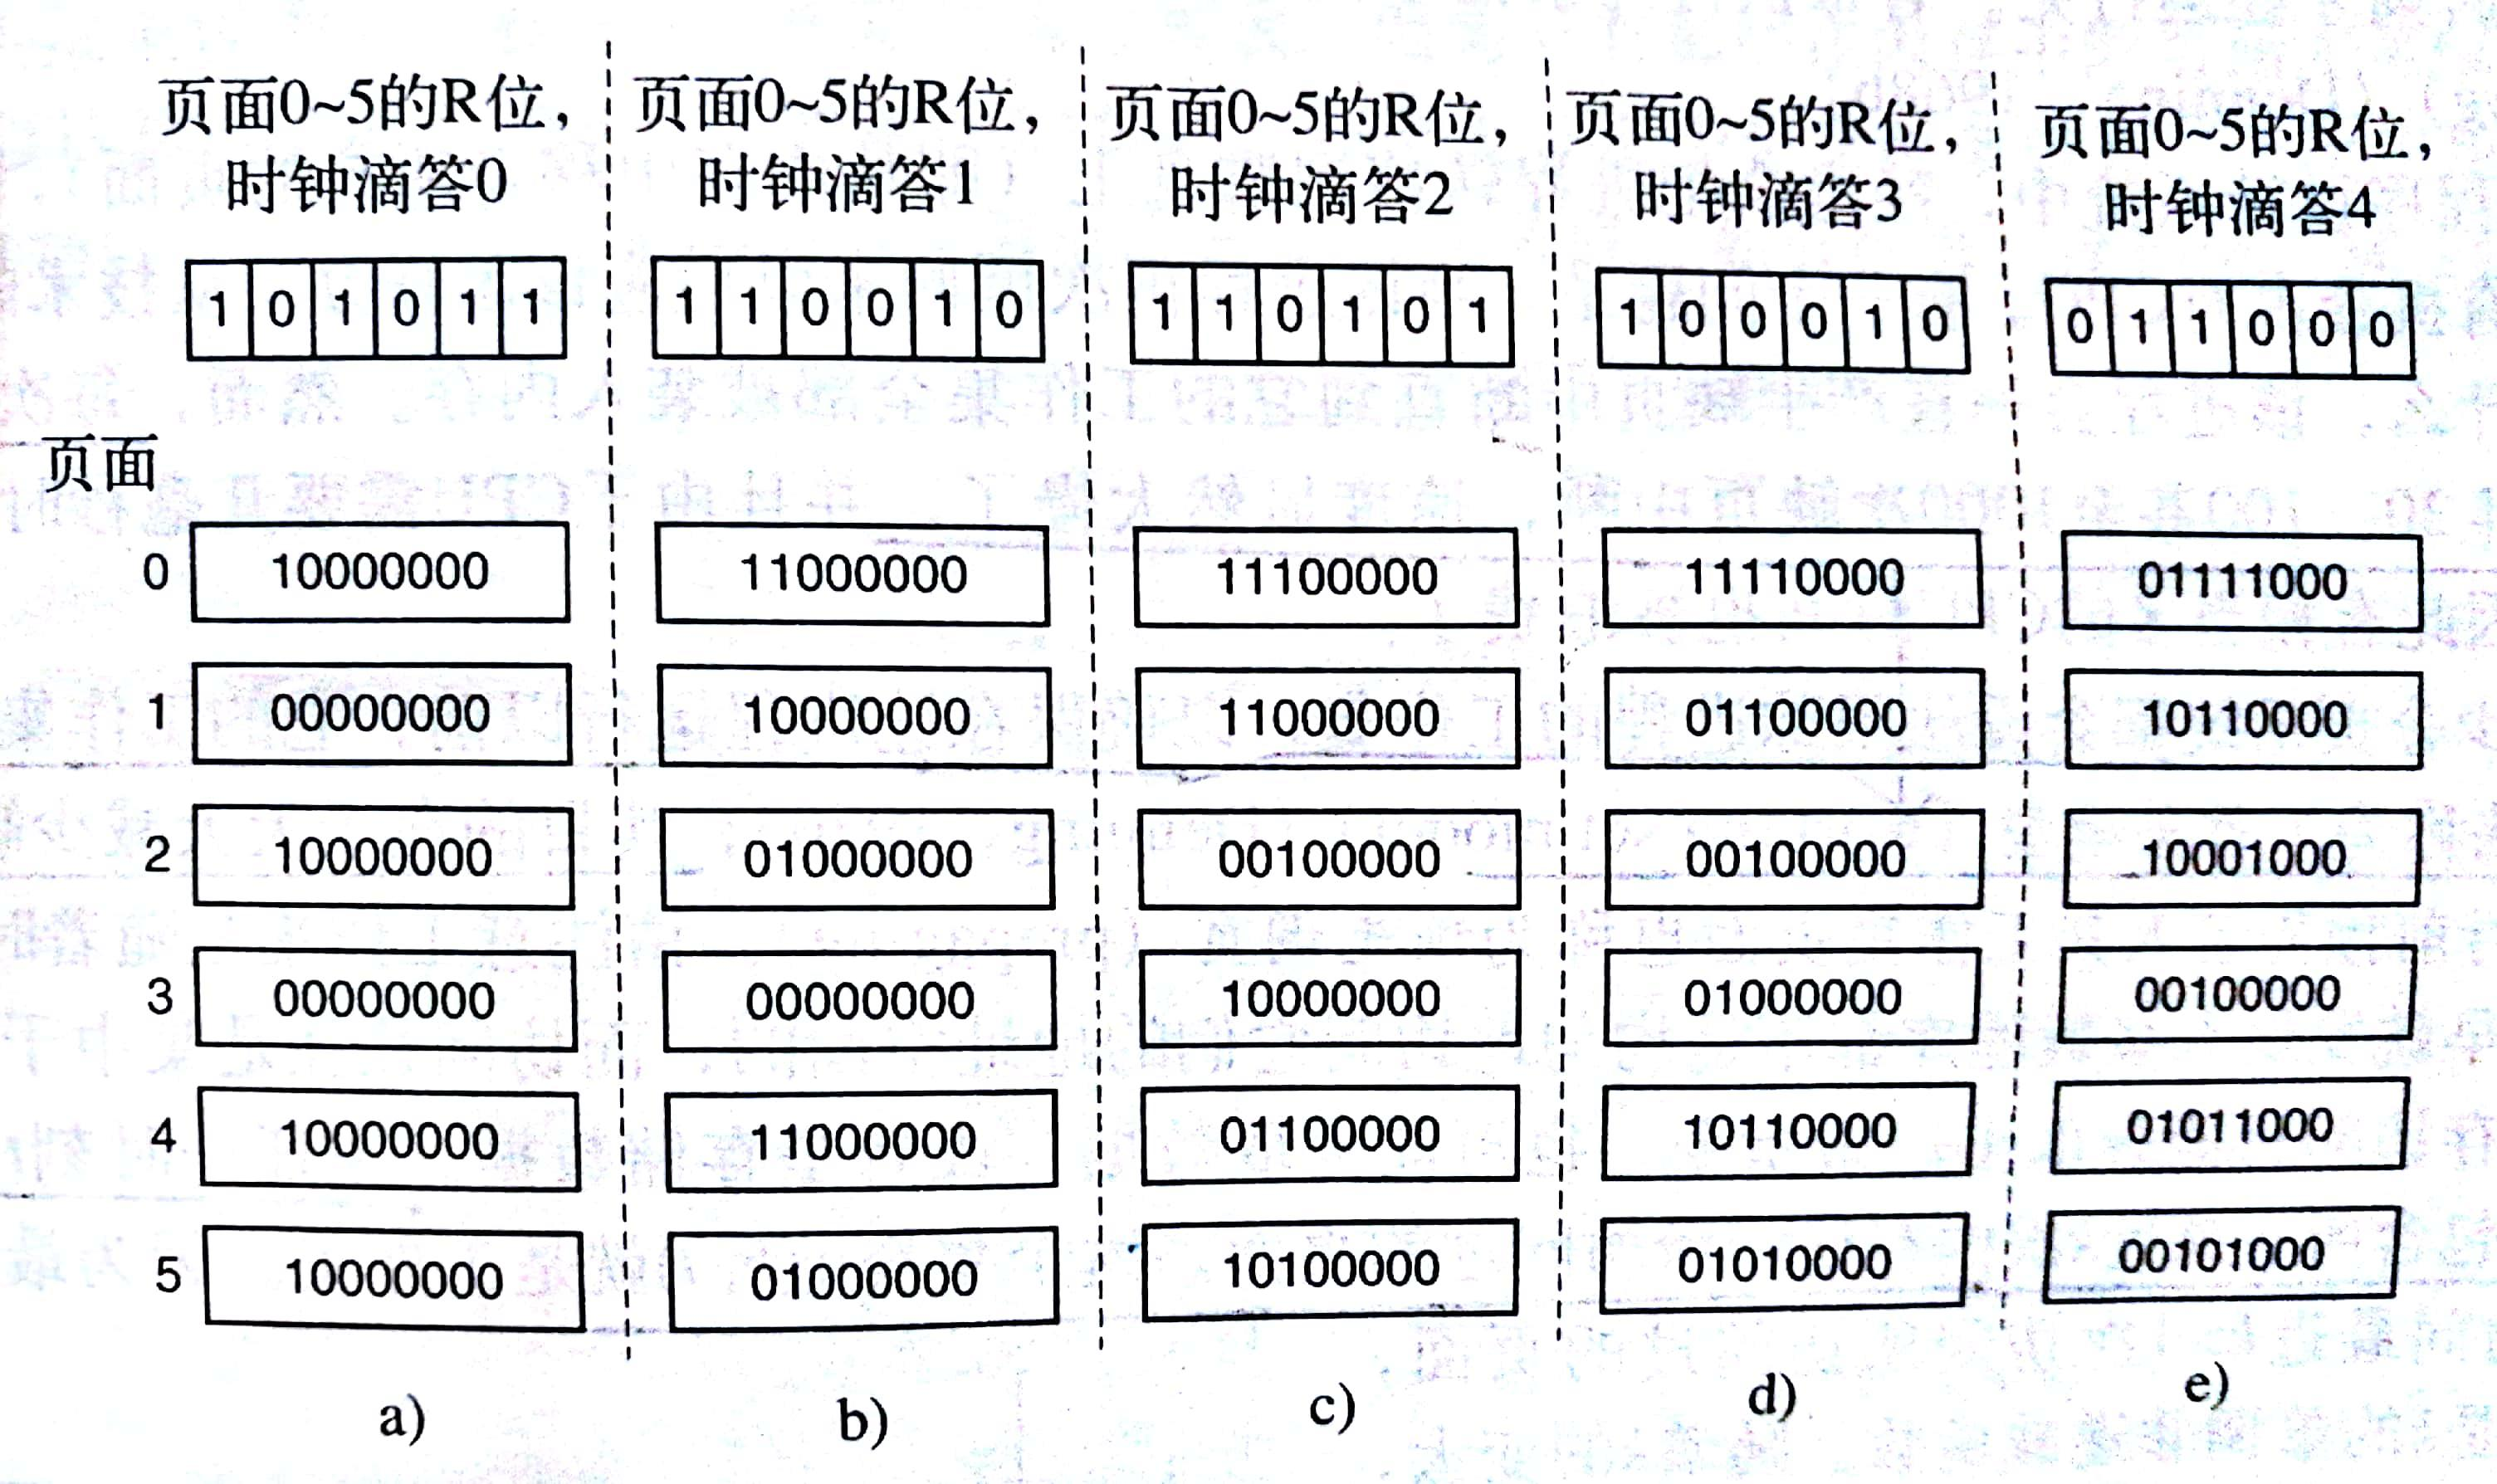
\includegraphics[scale = 0.1]{assets/ModernOperatingSystems_0ac67.png}
		      \caption{老化算法 , 6个页面在5个时钟滴答的情况}
	      \end{figure}

	\item 工作集页面置换算法\\
	      一个进程当前正在使用的集合称为 \textbf{工作集}\\
	      进程在运行以前, 工作集已经在内存中了,那么就可以大大减少缺页中断率
	      \begin{itemize}
		      \item 维护进程最近k次内存访问的页面为工作集 , 但是维护的开销大
		      \item 近似: 不向后找k次内存访问, 而是考虑执行时间:在过去$\tau$秒实际运行时间中它所访问过的页面的集合
		      \item 找出不在工作集的页面替换掉
		      \item 没有可淘汰的页面就随机淘汰
	      \end{itemize}
	      \begin{figure}[H]
		      \centering
		      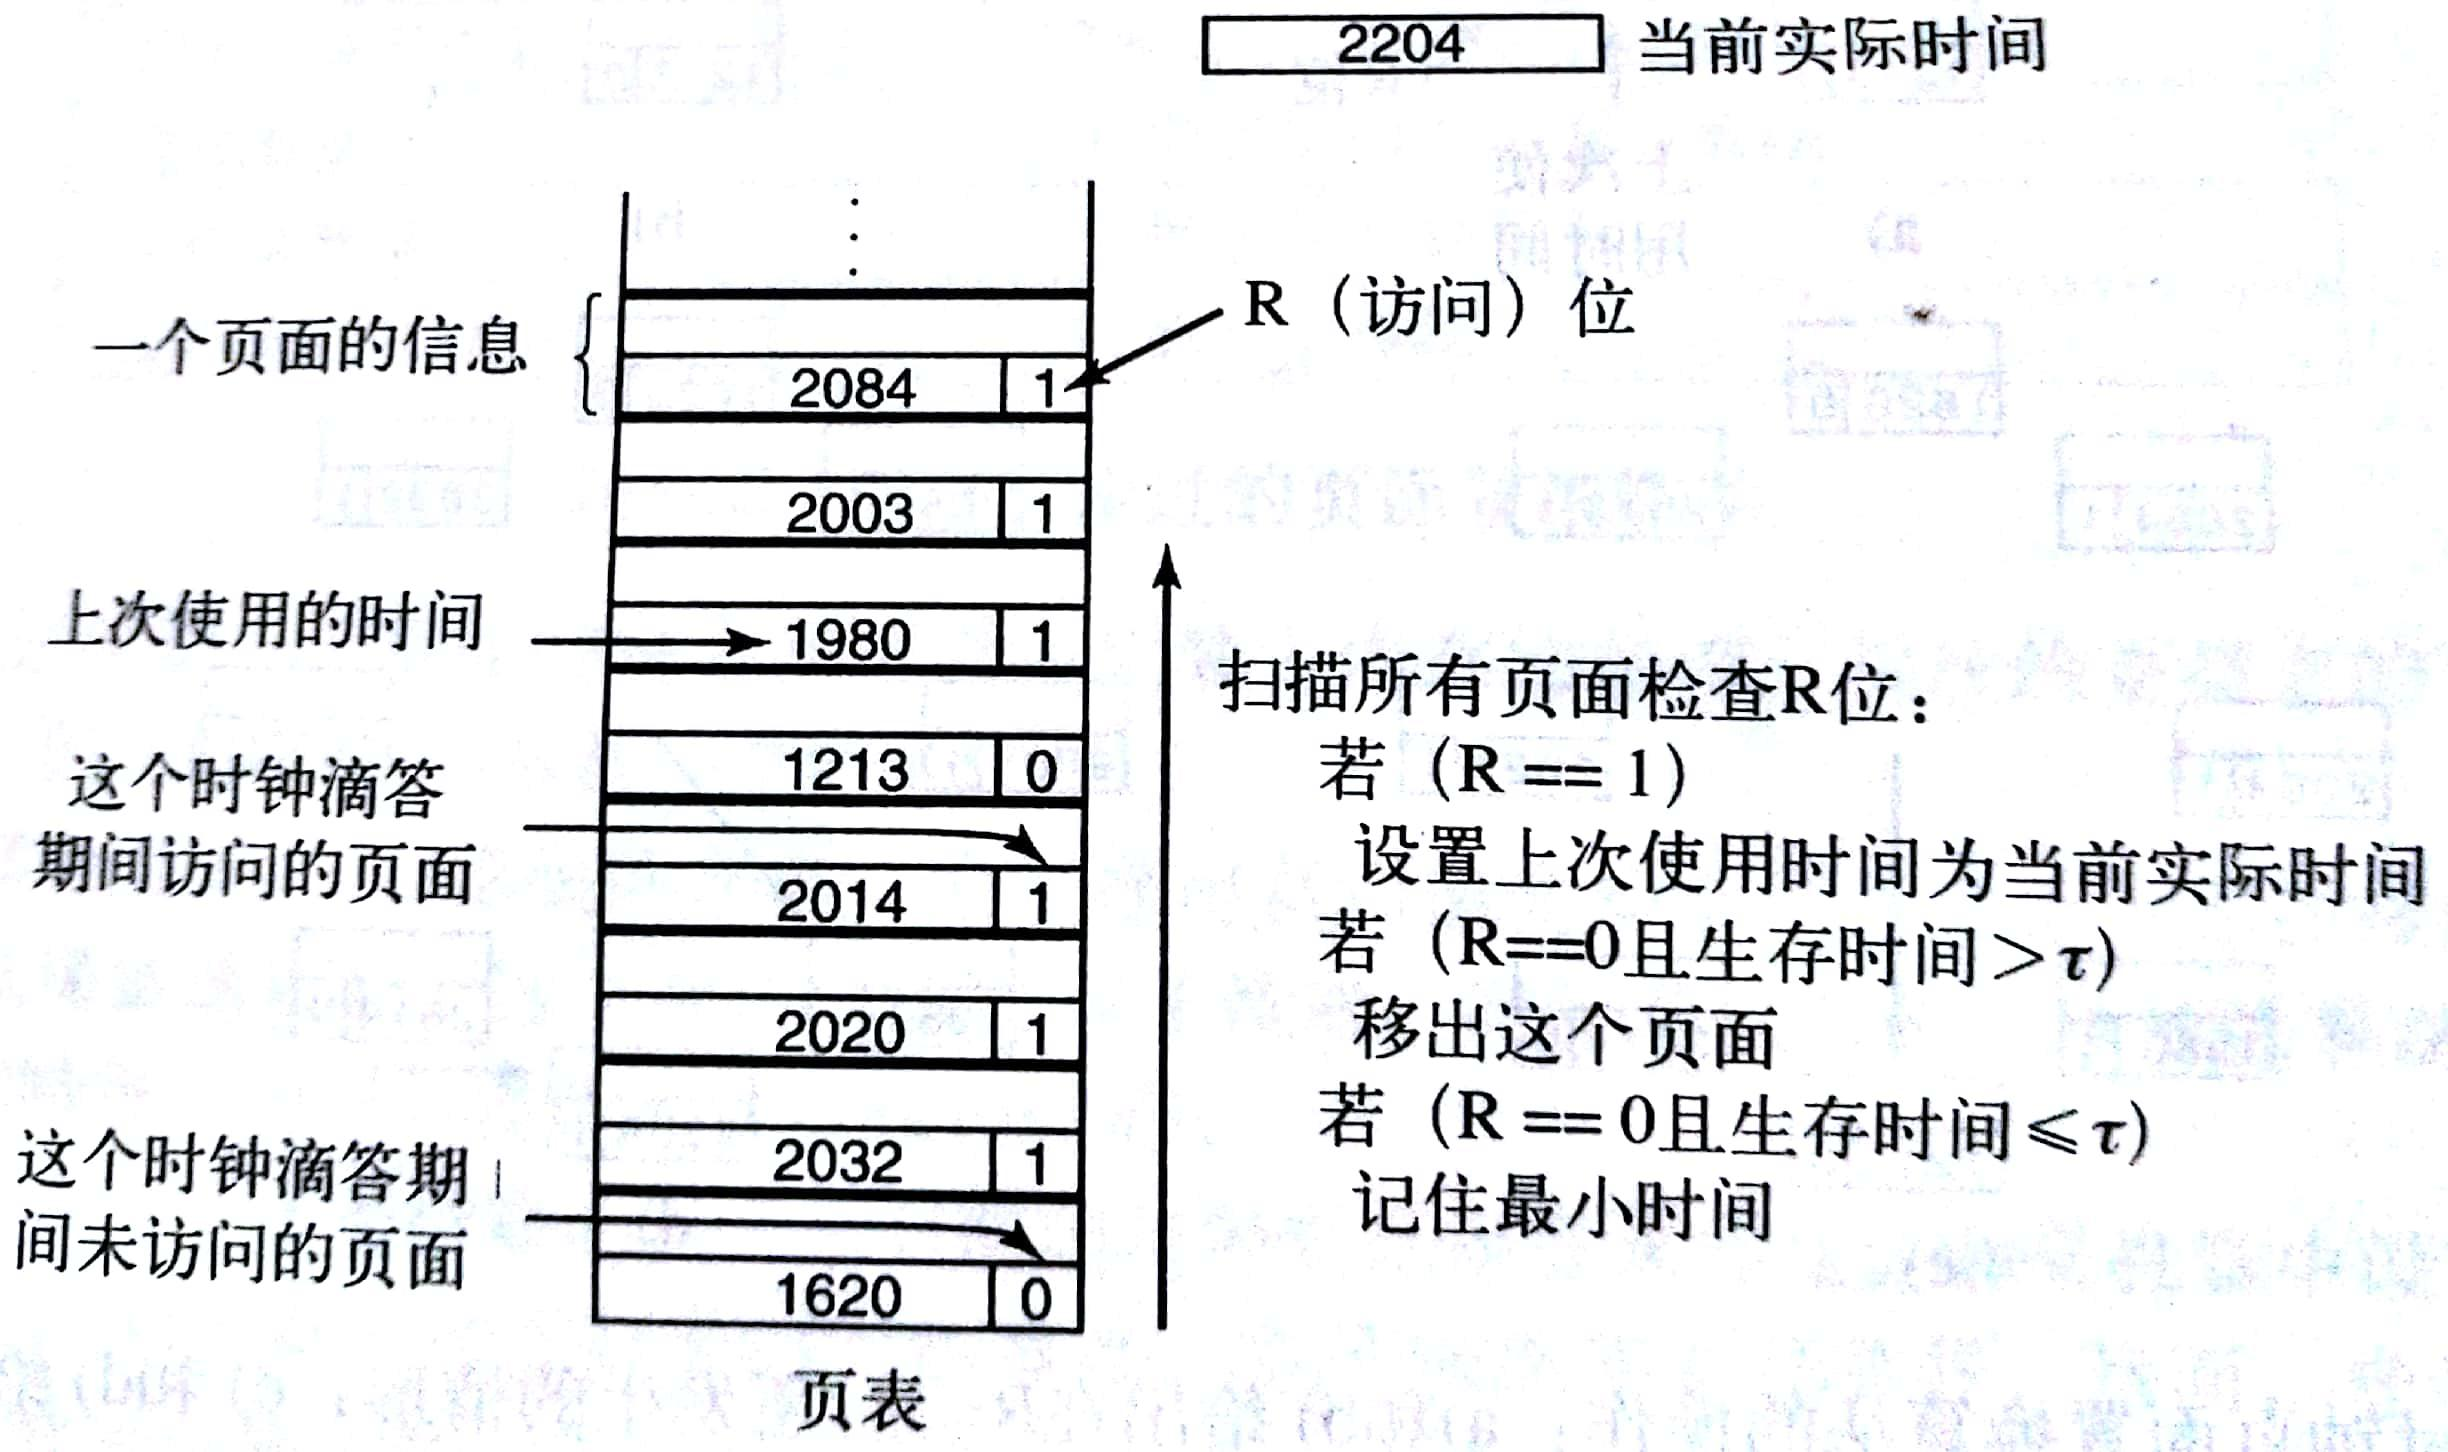
\includegraphics[scale = 0.1]{assets/ModernOperatingSystems_6bdcb.png}
		      \caption{工作集算法}
	      \end{figure}
	      和NRU有点像 , 但是它是通过R位来判断是否在时钟滴答更新时间 , 和计算时间决定是否淘汰
	\item 工作集时钟页面置换算法
	      \begin{itemize}
		      \item 每次缺页中断,指针指向的页面
		      \item 如果R = 1, 该页面在当前时钟地方访问过, 不适合淘汰 , 置R为0 ,更新时间 ,  指针指向下一个页面
		      \item 如果R = 0 , 计算$\tau$ 看是否能淘汰
		      \item 如果可淘汰, 但该页面被修改需要写回 , 则指针后移,继续寻找 , 避免磁盘I/O
		      \item 定义每个时钟滴答最大只允许写回n个页面
		      \item 当指针回到起点 , 如果进行了一次写操作 , 那么后续肯定有干净的页面可以替换
		      \item 当回到起点是 ,没有进行一次写回 ,说明所有页面都在工作集中 , 随机置换一个干净的页面(往后扫描干净的页面 ,置换 , 没有干净的页面 , 就把当前的页面写回再替换)
	      \end{itemize}
\end{itemize}

\begin{figure}[H]
	\centering
	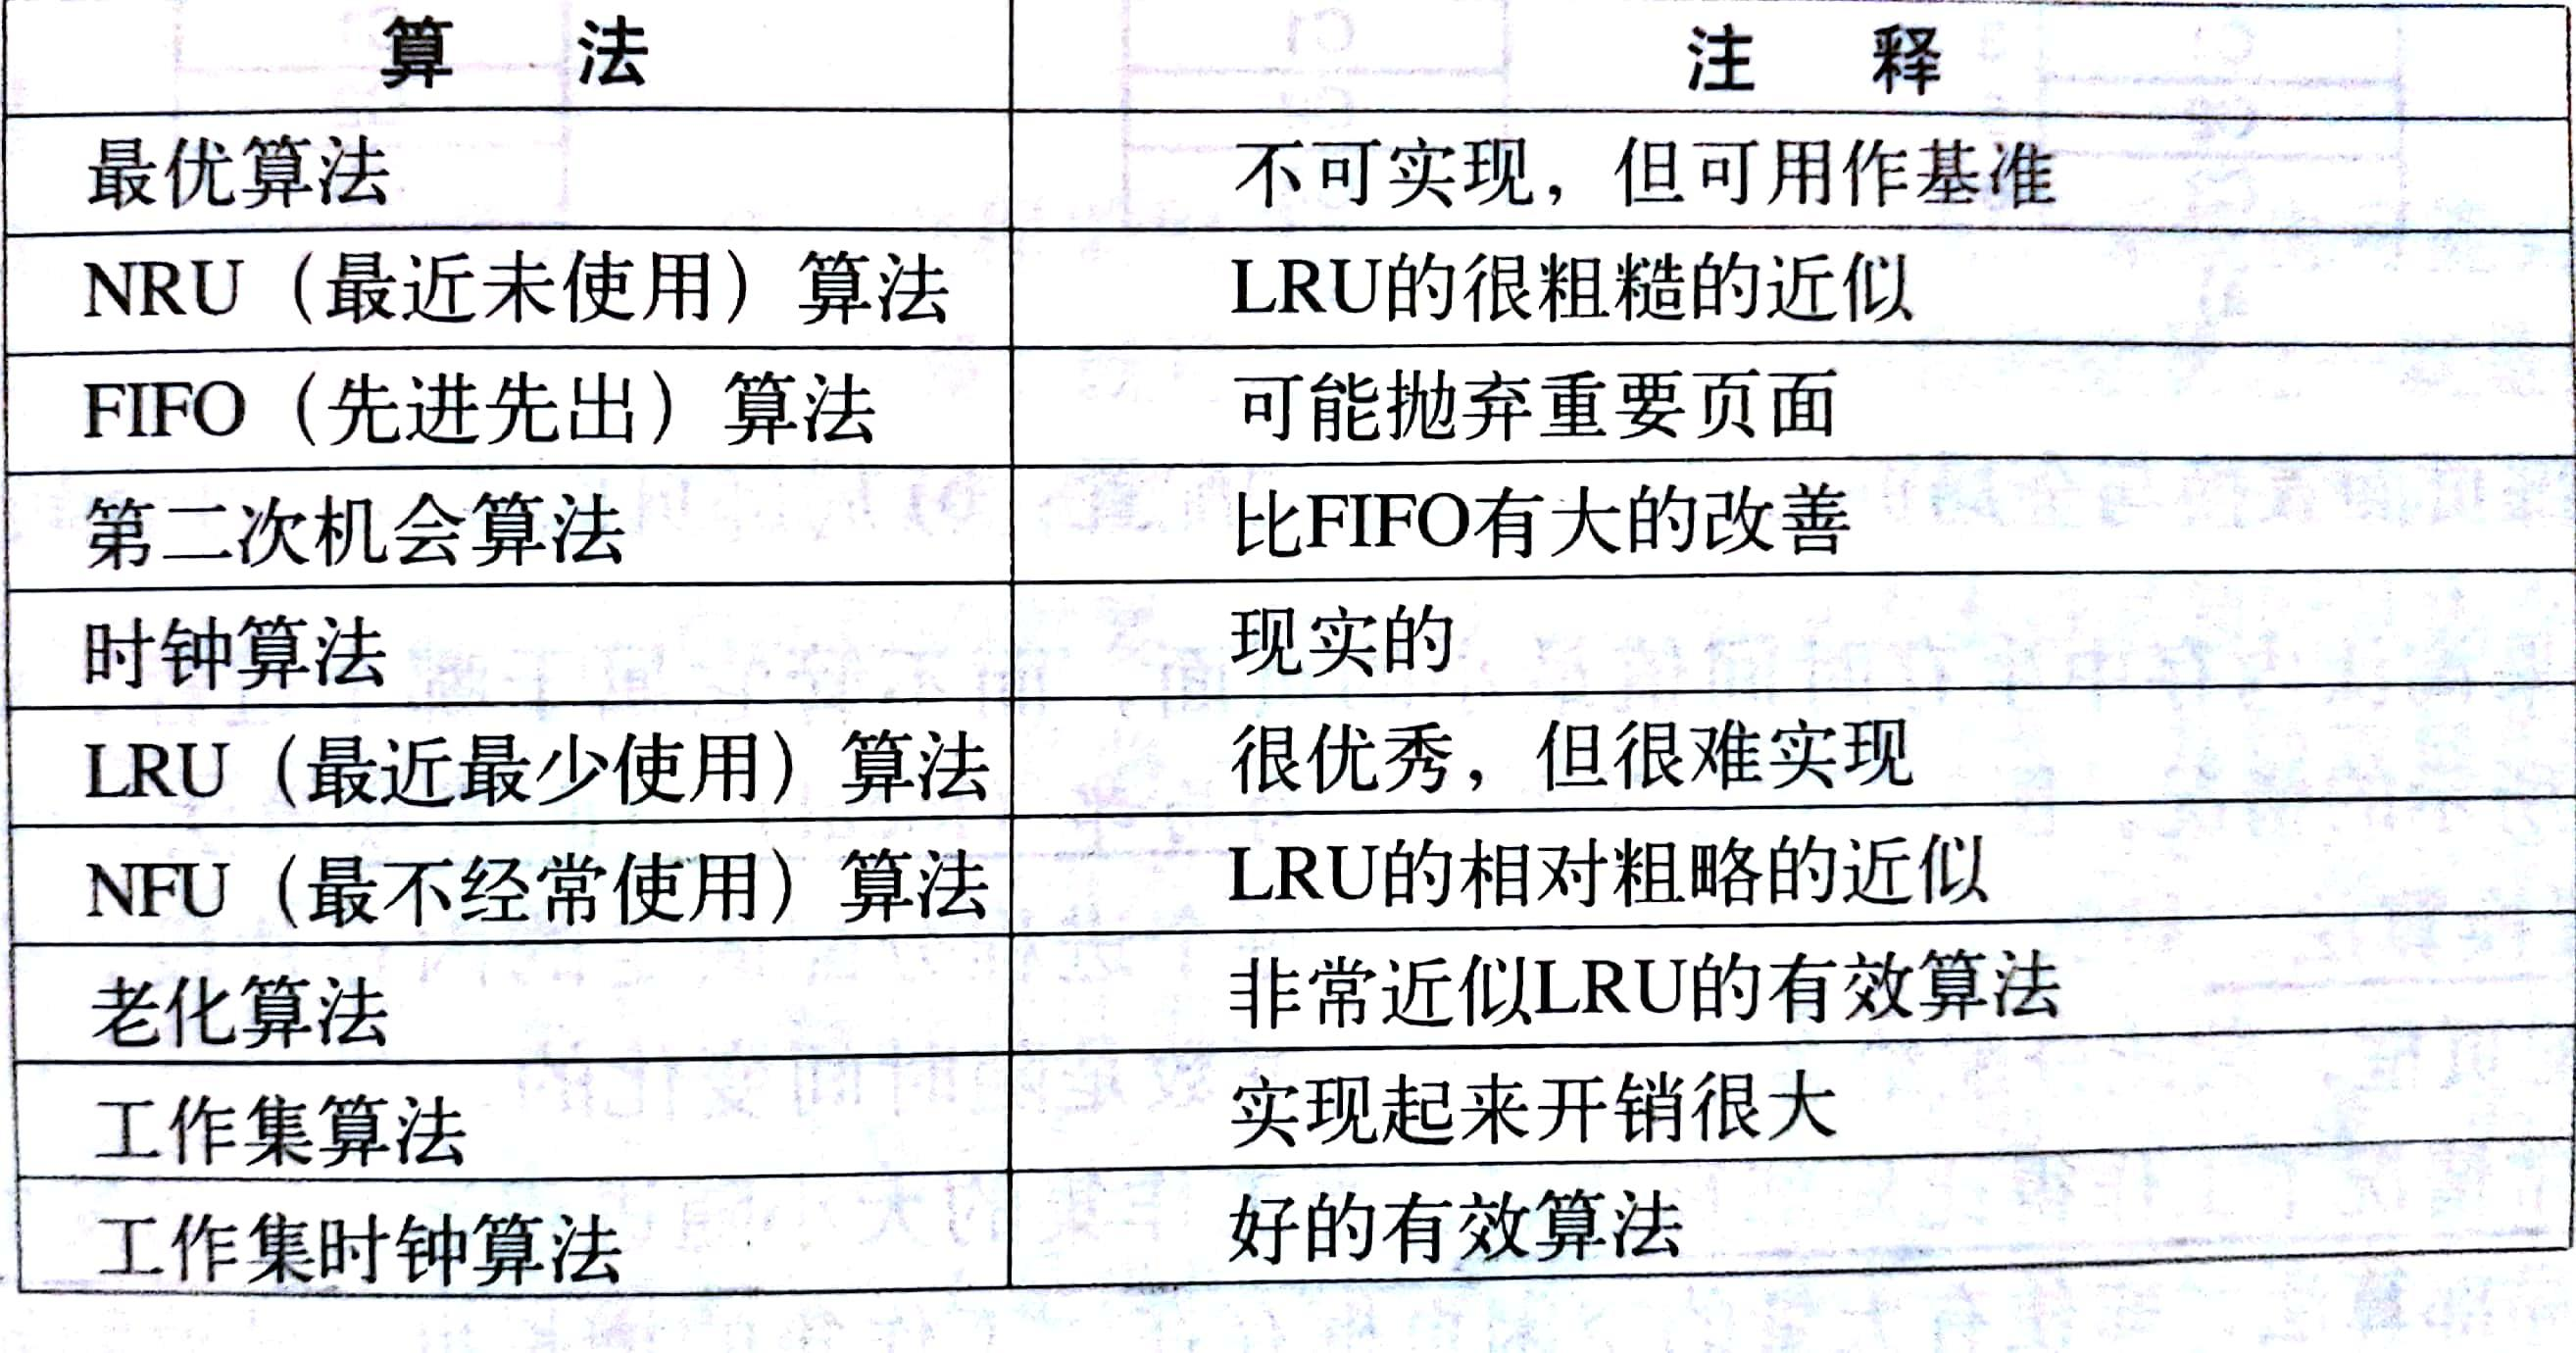
\includegraphics[scale = 0.1]{assets/ModernOperatingSystems_22227.png}
	\caption{小结:最好的算法是老化算法和时钟工作集算法}
\end{figure}

\subsubsection{分页系统设计问题}
\begin{itemize}
	\item 局部分配策略和全局分配策略\\
	      全局分配 : 淘汰生存值最小的页面 , 不管它属于哪个进程\\
	      全局算法在通常情况下工作得比局部算法好,当工作集的大小随进程运行时间发生变化时这种现象更加明显
	      管理内存动态分配的一种方法 : PFF ,Page Fault Frequency , 缺页中断率算法 
	\item 负载控制 : 工作集超出内存容量, 可能发生颠簸\\
	      解决方案是从内存中去掉一些进程
	\item 页面大小 : 页面过大, 则平均情况最后一个页面有一半是空的 , 多余的空间就被浪费,称为 \textbf{内部碎片}\\
	      大页面使更多没有用的程序保留在内存中\\
	      小页面意味着更大的页表\\
	      求最佳的页面大小 : 最小化页表开销+内部碎片 之和
	      % \begin{figure}[H]
	      %   \centering
	      %   \includegraphics[scale = 0.3]{}
	      %   \caption{最佳页面大小数学分析}
	      % \end{figure}
	\item 数据空间和指令空间分离 : 即各自一个地址空间
	\item 共享页面 : 页面共享, 写时复制
	\item 共享库 , 动态链接库(Windows) , 使用其他粒度代替单个页面共享
	\item 内存映射文件 : 共享库更加通用机制
	\paragraph{思想}:进程可以通过发起一个系统调用 , 将一个文件映射到其虚拟地址空间的一部分;在多数实现中 , 在映射共享的页面时不会实际读入页面的内容 ,而是在访问页面时才会被每次一页地读入 , 磁盘文件被当作后备存储。\\
	当进程退出或显式地解除文件映射时,  所有被改动的页面会被写回到文件中\\
	内存映射文件可以把一个文件当作一个内存中的大字符数组来访问, 而不用通过读写操作来访问这个文件\\
	如果两个或两个以上的进程同时映射了同一个文件,他们就可以通过共享内存来通信
	\item 清除策略 : 为保证有足够的空闲页框, 很多分页系统被一个称为 \textbf{守护进程 paging daemon} 的后台进程 , 它在打多数时候睡眠、但定期被唤醒以检查内存的状态;\\
	如果空闲页框过少, 分页守护进程通过预定的页面置换算法选择页面换出内存\\
	当需要使用一个已被淘汰的页面时, 如果该页框还没有被覆盖, 将其从空闲页框缓冲池中移出即可恢复该页面
	\paragraph{一种实现方式} 使用双指针时钟 ,前指针由分页守护进程控制 ,  当它指向一个脏页面时 , 就把该页面写回磁盘 ,前指正向前移动 ; 当它指向干净页面时, 直接向前移动 ;\\
	后指针用于页面置换 , 就像标准时钟算法中一样	
	\item 虚拟内存接口 : 当目前为止,所有的讨论都假定虚拟内存对进程和程序员都是透明的 ; 现在希望程序员可以对内存映射进行控制, 并可以通过非常规的方法来增强程序的行为
	\begin{itemize}
		\item 允许两个或者多个进程共享同一部分内存 : 如果程序可以对内存区域进行命名 , 那么就可以实现内存共享
		\item 页面共享也可用来实现高性能的消息传递系统 : 一般系统传递消息的时候,数据库被从一个地址空间复制到另一个地址空间,开销很大 ; 如果进程可以控制他们的页面映射, 就可以发送进程清楚那些包含消息的页面映射, 而接收进程把他们映射进来;\\
		这里就只需要复制页面的名字,而不需要复制所有数据
		\item 分布式共享内存 : 允许网络上的多个进程共享一个页面集合 
	\end{itemize}
\end{itemize}

\subsubsection{实现问题}
与分页有关的4个工作:
\begin{itemize}
	\item 创建新的进程 : 创建一个新进程时, 想为这个进程创建一个页表,操作系统在内存中为其分配空间并进行初始化
	\item 进程执行时 : 必须为新进程重置MMU , 刷新TLB , 以清除以前的进程遗留的痕迹;新进程的页表必须成为当前页表
	\item 缺页中断发生时 
	\item 进程退出时 : 操作系统必须释放进程的页表 、页面和页面在硬盘上所占的空间\\如果某些页面时和其他进程共享的,当最后一个使用它们的进程终止的时候,才可以释放内存和磁盘上的页面
\end{itemize}

\paragraph{缺页中断处理}

\begin{itemize}
	\item 硬件陷入内核, 在堆栈中保存程序计数器;\\
	大多数机器将当前各种状态信息保存在特殊的CPU寄存器中
	\item 启动一个汇编代码例程保存 \textbf{保存通用寄存器和其他易失的信息} 以免被操作系统破坏 ; 这个例程将操作系统作为一个函数调用
	\item 当操作系统发现一个缺页中断时, 尝试发现需要哪个虚拟页面。
	\item 一旦知道了发生缺页中断的虚拟地址 , 操作系统检查这个地址是否有效,并检查存取与保护是否一致。\\
	如果不一致,向进程发出一个信号或杀掉该进程\\
	如果地址有效且没有保护错误发生,系统则检测是否有空闲页框;没有则执行页面置换算法寻找一个页面来淘汰
	\item 如果选择的页面是脏页面 , 安排该页写回磁盘, 并发生一次上下文切换,挂起产生缺页中断的进程,让其他进程运行直至传输结束。该页面被标记为忙, 以免因为其他原因而被其他进程占用
	\item 一旦页面干净后 , 操作系统查找所需页面在磁盘上的地址,通过磁盘操作将其装入。该页面被装入后 , 发生缺页中断的进程仍处于挂起状态
	\item 当磁盘中断发生时, 表明该页已经被装入, 页表已经更新可以反映它的位置 , 页框也被标记为正常状态
	\item 恢复发生缺页中断指令以前的状态, 程序计数器重新指向这条指令
	\item 调度引起缺页中断的进程 , 操作系统返回调用它的汇编语言例程
	\item 该例程恢复寄存器和其他状态信息 , 返回到用户空间继续执行 , 就好像缺页中断没有发生一样
\end{itemize}

\paragraph{指令备份} 
% 当程序访问不在内存的页面时, 引起缺页中断的指令会半途停止并引发操作系统的缺陷
喵喵喵


\paragraph{锁定内存中的页面} 
在等待I/O完成时,该进程被挂起 , 另一个进程被允许运行 ,而这个进程产生一个缺页中断

如果是全局的分页算法,包含I/O缓冲区的页面有几率被换出内存

\paragraph{解决办法}所注正则做I/O的内存中的页面以保证它不会被移除内存 , 或在内存缓冲区中完成所有的I/O操作, 然后再将其复制到用户界面

\paragraph{后备存储}
我们已经知道如何选择换出内存的页面 , 但是却没有讨论当前页面被换出时会存放在磁盘上的哪个位置

在磁盘上设置特殊的交换分区 , 甚至从文件系统划分一块独立的磁盘(以平衡I/O负载)

\paragraph{有两种分配方案}
\begin{itemize}
	
	\item 每个进程均占用一块外存空间,这个空间大小和进程一样大
	
	进程结束之后 , 会释放其磁盘上的交换区,交换分区以空闲块列表的形式组织(是文件空闲块而不是内存空闲块)
	
	\item 实现什么有不分配 , 在页面换出时为其分配空间 , 并在换入时回收磁盘空间,这样内存中的进程不必固定于任何一个交换空间
\end{itemize}

\begin{figure}[H]
	\centering
	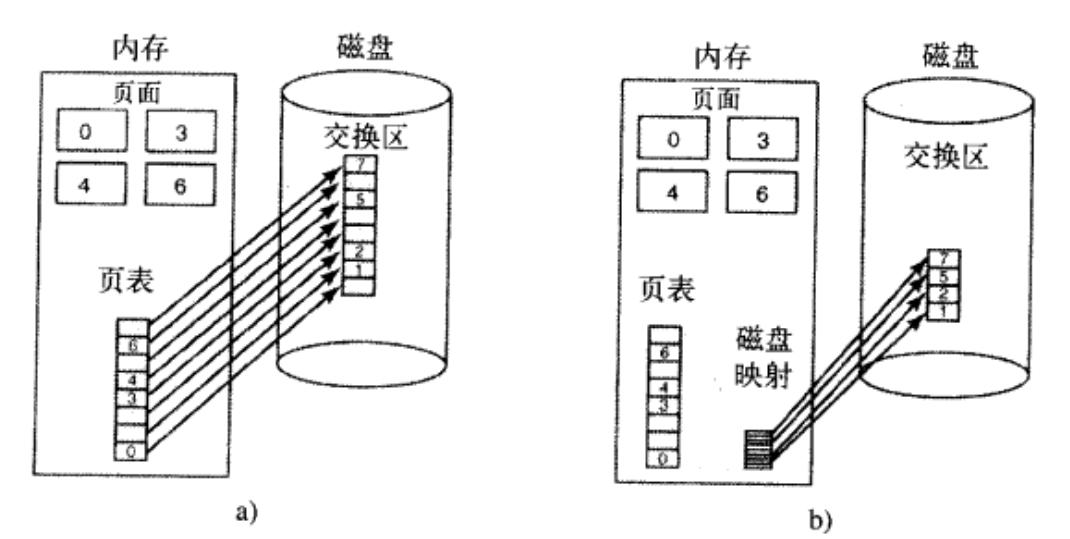
\includegraphics[scale = 0.4]{assets/ModernOperatingSystems/2018-01-10-23-15-08.png}
	\caption{a) 对静态交换区分页 b)动态备份页面}
\end{figure}

但是,并不能总能够实现有固定的交换分区(磁盘空间不够) , 对于可执行文件 , 由于程序正文通常是只读 , 当内存紧张、程序也不得不移出内存时,尽管丢弃他们


\paragraph{策略和机制分离}
\subparagraph{策略和机制分离下的缺页中断处理}
把策略从机制中分离出来 , 此情况下 , 存储管理系统被分为3个部分
\begin{itemize}
	\item 一个底层的MMU处理程序
	\item 一个作为内核一部分的缺页中断处理程序
	\item 一个运行在用户空间中的外部页面调度程序
\end{itemize}

策略主要由作为用户进程运行的外部页面调度程序决定

\begin{figure}[H]
	\centering
	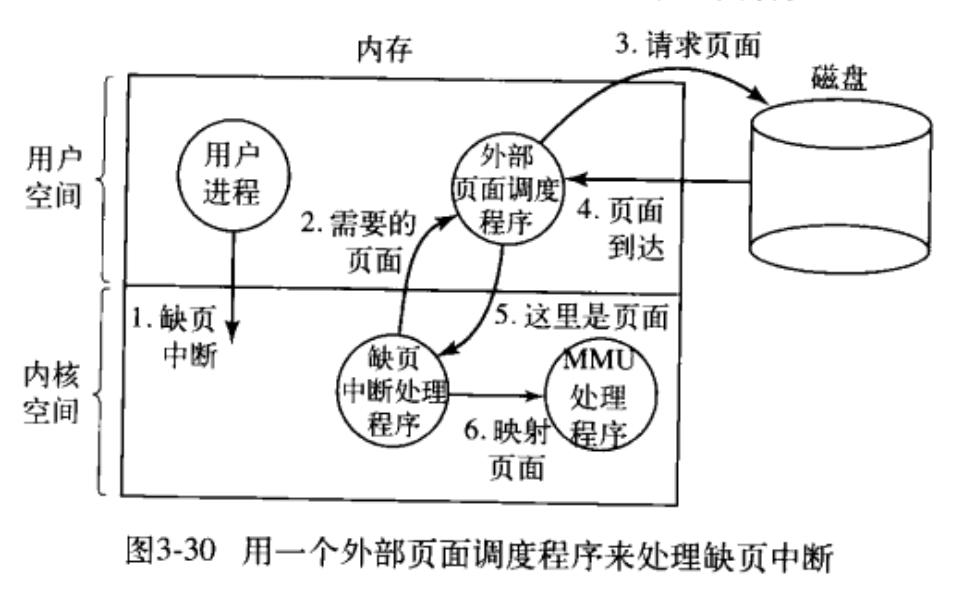
\includegraphics[scale = 0.5]{assets/ModernOperatingSystems/2018-01-10-23-19-09.png}
	\caption{用一个外部页面调度程序来处理缺页中断}
\end{figure}

\paragraph{过程:}
\begin{itemize}
	\item 缺页中断处理程序找出哪个虚拟页面 , 并发送一条消息给外部页面调度程序告诉它发生了什么问题
	\item 外部页面调度程序从磁盘中读入所需的页面, 把他复制到自己的地址空间的某一位置
	\item 然后告诉缺页中断处理程序该页面的位置 
	\item 缺页中断处理程序从外部页面调度程序的地址空间中清除该页面的映射 , 然后请求MMU处理程序把它放在用户地址空间的正确位置, 随后就可以启动用户进程了
\end{itemize}

\paragraph{优缺点}
这种实现的主要有点是有更多的模块化代码和更好的适应性 

主要缺点是由于多次交叉用户-内核边界引起的额外开销, 以及系统模块间消息传递所造成的额外开销


\subsection{分段}
到目前为止, 我们讨论的地址都是一维的,程序员需要控制地址空间的分配; 我们希望把程序员功从管理表的扩张和收缩的工作中释放出来

\paragraph{解决方案} 分段

因为每个段都构成了一个独立的地址空间 ,所以他们可以独立地增长或减小而不影响到其他的段

\begin{figure}[H]
	\centering
	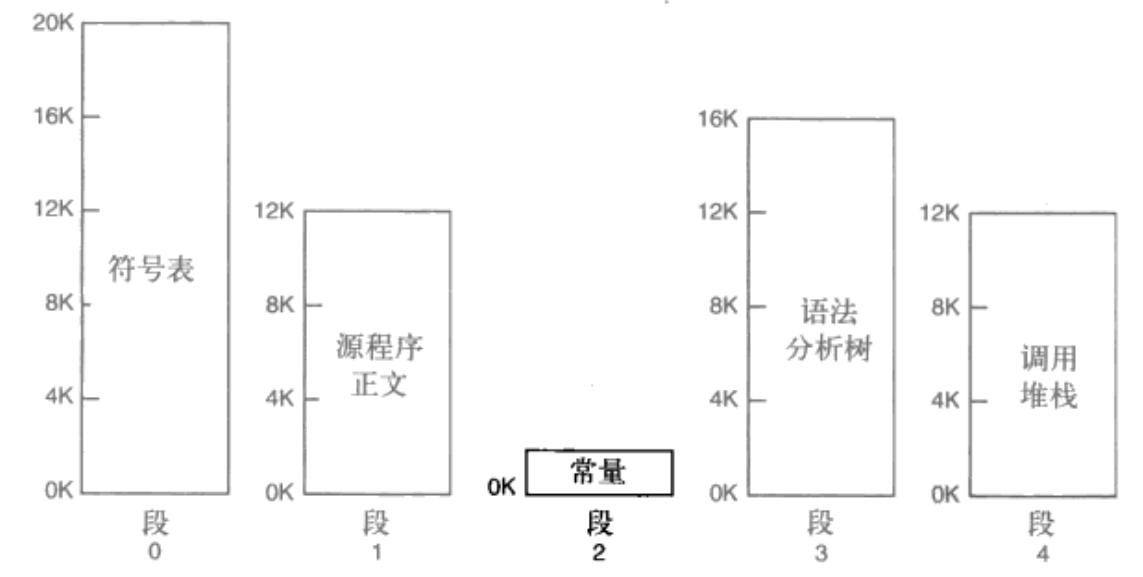
\includegraphics[scale = 0.4]{assets/ModernOperatingSystems/2018-01-10-23-27-27.png}
	\caption{分段存储管理, 每一个段都可以独立地增大或减小而不会影响其他段}
\end{figure}

\paragraph{分段和分页的比较} 
\begin{figure}[H]
	\centering
	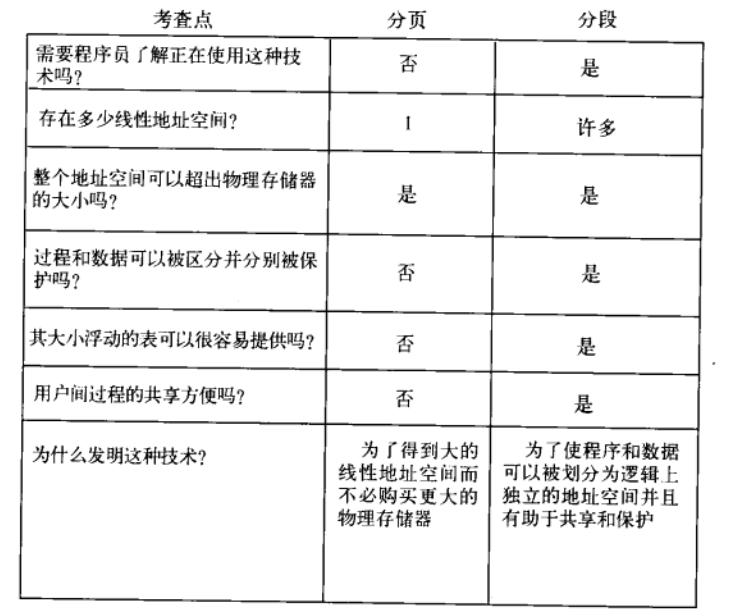
\includegraphics[scale = 0.5]{assets/ModernOperatingSystems/2018-01-10-23-28-29.png}
	\caption{分段和分页的比较}
\end{figure}

\paragraph{纯分段实现}
页面是定长的,而段不是 , 因此 , 纯分段的实现 ,在运行一段时间后, 会产生很多空闲区 , 需要通过内存紧缩来解决

\subsection{分段和分页结合 : MULTICS}
如果一个段比较大, 把它整个保存在内存中可能很不方便,甚至不可能 , 因此产生了 \textbf{段内分页} 的想法. 从而段内的地址不连续, 以缓解出分段模式下的碎片问题

每个MULTICS程序都有一个段表 , 每个段表对应一个描述符 , 段表本身也是一个段并被分页

\paragraph{MULTICS的地址的两个部分}段和段内地址,段内地址进一步分为页号和页内的字

\paragraph{执行的算法过程}为简单起见,忽略了描述符自己也分页的事实
\begin{itemize}
	\item 根据段号找到段描述符
	\item 检查该段的页表是否在内存中, 如果在 , 则找它的位置 , 如果不在 ,则产生一个段错误 ;如果访问违反了段的保护要求就发出一个越界错误
	\item 检查所请求虚拟页面的页表项, 如果该页面不在内存中 ,则产生一个缺页中断 , 如果在,则取出页面内存中的起始
	\item 将偏移量加到页面的起始地址 , 得到要访问的字在内存中的地址
	\item 最后进行读写操作
\end{itemize}

\subsection{分段和分页结合 : Intel Pentium} P135
Pentium 处理器中虚拟内存的核心是两张表: LDT Local descriptor table 局部描述符 和 GTD 全局描述符 

每个程序都有自己的LDT , 但是同一台计算机上的所有程序共享一个GDT 

LDT描述局部于每个程序的段 , 包括其代码  数据,堆栈等 

GDT描述系统段 , 包括操作系统本身

\paragraph{线性地址转换}
\begin{figure}[H]
	\centering
	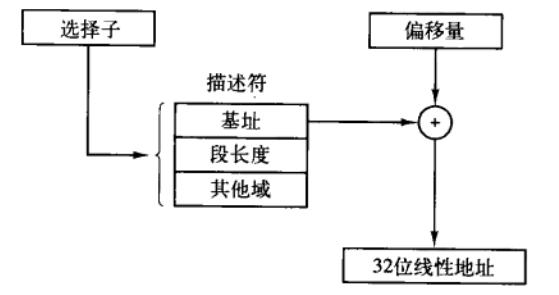
\includegraphics[scale = 0.5]{assets/ModernOperatingSystems/2018-01-10-23-41-30.png}
	\caption{(选择子, 偏移量)对转换为线性地址}
\end{figure}

 如果允许分页,线性地址将通过页表映射到物理地址
 
 \paragraph{使用了一种两级映射 , 以便在段小的是减小页表大小}
 \begin{figure}[H]
	 \centering
	 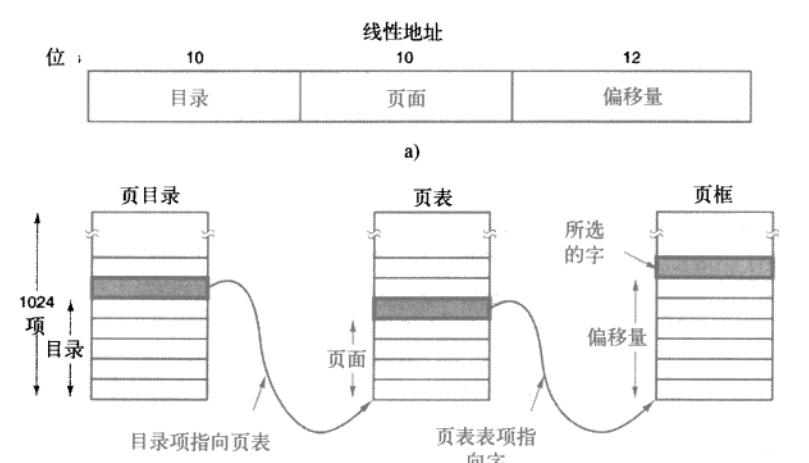
\includegraphics[scale = 0.5]{assets/ModernOperatingSystems/2018-01-10-23-45-29.png}
	 \caption{线性地址到物理地址的映射}
 \end{figure}

 线性地址被分为3个域:目录、页面和偏移量

\begin{itemize}
	\item 目录域被作为索引在页目录中找到指向正确页表的指正
	\item 随后页面域被用作索引在页表中找到页框的物理地址
	\item 最后偏移量被加到页框上得到需要的字节或字的物理地址
\end{itemize}
 
\section{文件系统}

\paragraph{文件系统的动机}
存储容量受内存空间大小的限制 , 而且进程终止是信息有随之丢失

\paragraph{长期存储信息的3个基本要求} 能存储大量信息 ; 使用信息的进程终止时,信息仍旧存在 ; 必须能使多个进程并发存取有关信息

文件是进程创建的信息逻辑单元 , 每个文件可以看成是一种地址空间

操作系统中处理文件的部分称为 \textbf{文件系统}

\subsection{文件}
\subsubsection{文件命名} 
现代操作系统中,一般使用1-8个字母组成的字符串作为合法的文件名, 也允许有数字或一些特殊字符

有的文件系统区分大小写

\subsubsection{文件结构} 
文件可以有多种构造方式 , 以下是常见的3种:
\begin{figure}[H]
	\centering
	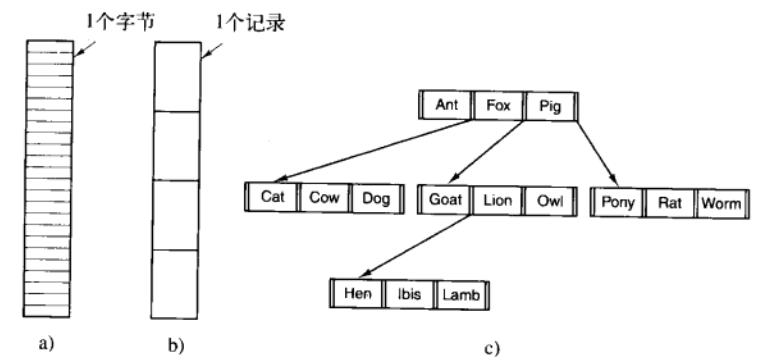
\includegraphics[scale = 0.5]{assets/ModernOperatingSystems/2018-01-10-23-55-30.png}
	\caption{3种文件结构 : a)字节序列 ; b)记录序列 ; c)树}
\end{figure}

\begin{itemize}
	\item 字节序列 : 文件是一种无结构的字节序列 , 操作系统事实上不知道也不关心文件内容是什么 , 操作系统所见到的就是字节  其任何含义只在用户程序中解释, UNIX 和 WINDOWS 都采用这种方法
	\item 记录序列 : 文件具有固定长度记录的序列, 每个记录都有其内部结构, 其思想是:读操作返回一个记录, 而写操作重写或追加一个记录
	\item 树 : 文件由一棵记录树构成,每个记录并不具备同样长度 , 而记录的固定位置上有一个键字段, 这个树按键字段排序 , 从而可以对特定的键进行快速查找(类似数据库的B树存储)
\end{itemize}

\subsubsection{文件类型} 
UNIX和WINDOWS都有普通文件和目录 , UNIX还有字符特殊文件和块特殊文件

普通文件分为ASCII文件和二进制文件

二进制文件具有一定的内部结构,使用该文件的程序才了解这种结构

\paragraph{魔数} UNIX可执行文件的文件头以 \textbf{魔数} 开始 , 表明该文件是一个可执行文件(防止非这种格式的文件偶然运行)

\subsubsection{文件存取} 
\paragraph{两种文件存取方式} 顺序存取 、 随机存取

\subsubsection{文件属性} 
操作系统还会保存其他与文件相关的信息,这些附加信息被称为 \textbf{文件属性} 或 \textbf{元数据}
\begin{figure}[H]
	\centering
	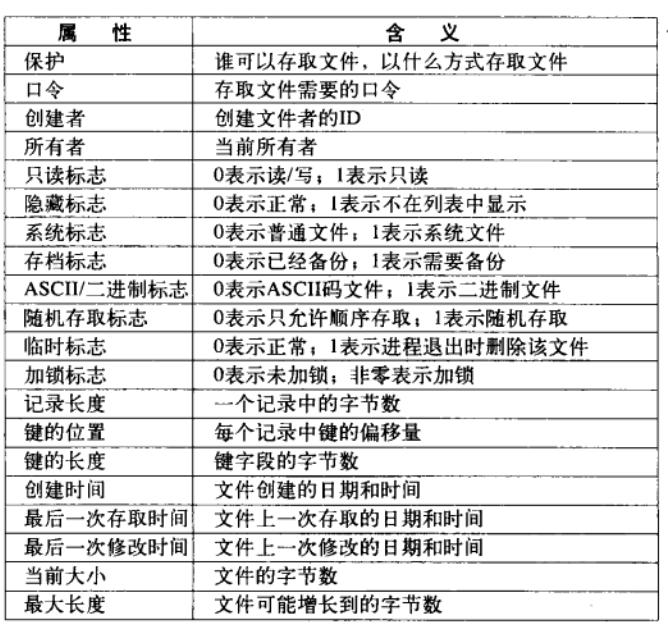
\includegraphics[scale = 0.5]{assets/ModernOperatingSystems/2018-01-11-00-08-45.png}
	\caption{一些常见的文件属性}
\end{figure}


\subsubsection{文件操作} 
使用文件的目的是存储信息并方便以后的检索

常见的文件操作有:create , delete , open ,close , read, write , ppend , seek , get attributes , set attributes , rename

\subsection{目录}
\textbf{目录分类} P150
\begin{itemize}
	\item 一级目录系统
	\item 层次目录系统
\end{itemize}

\textbf{路径} P151
\begin{itemize}
	\item 绝对路径
	\item 相对路径
\end{itemize}

\textbf{目录的操作} P152

\subsection{文件系统的实现}

\subsubsection{文件系统的布局} P153

\subsubsection{文件的实现} P154
\begin{itemize}
	\item 连续分配
	\item 链表分配
	\item 内存中采用表的链表分配
	\item i节点
\end{itemize}

\subsubsection{目录的实现}
\paragraph{目录的作用}:把 ASCII 文件名映射成定位文件数据所需的信息 ; 在读文件之前 , 必须打开文件 , 打开文件时 , 操作系统利用用户给出的路径名找到相应的目录项

\paragraph{在何处存放文件属性}
\begin{itemize}
	\item 直接放在目录项中
	\item 放在i节点中而不是目录项中 , 这样目录项弧更短 : 只有文件名和i节点号
\end{itemize}

\begin{figure}[H]
	\centering
	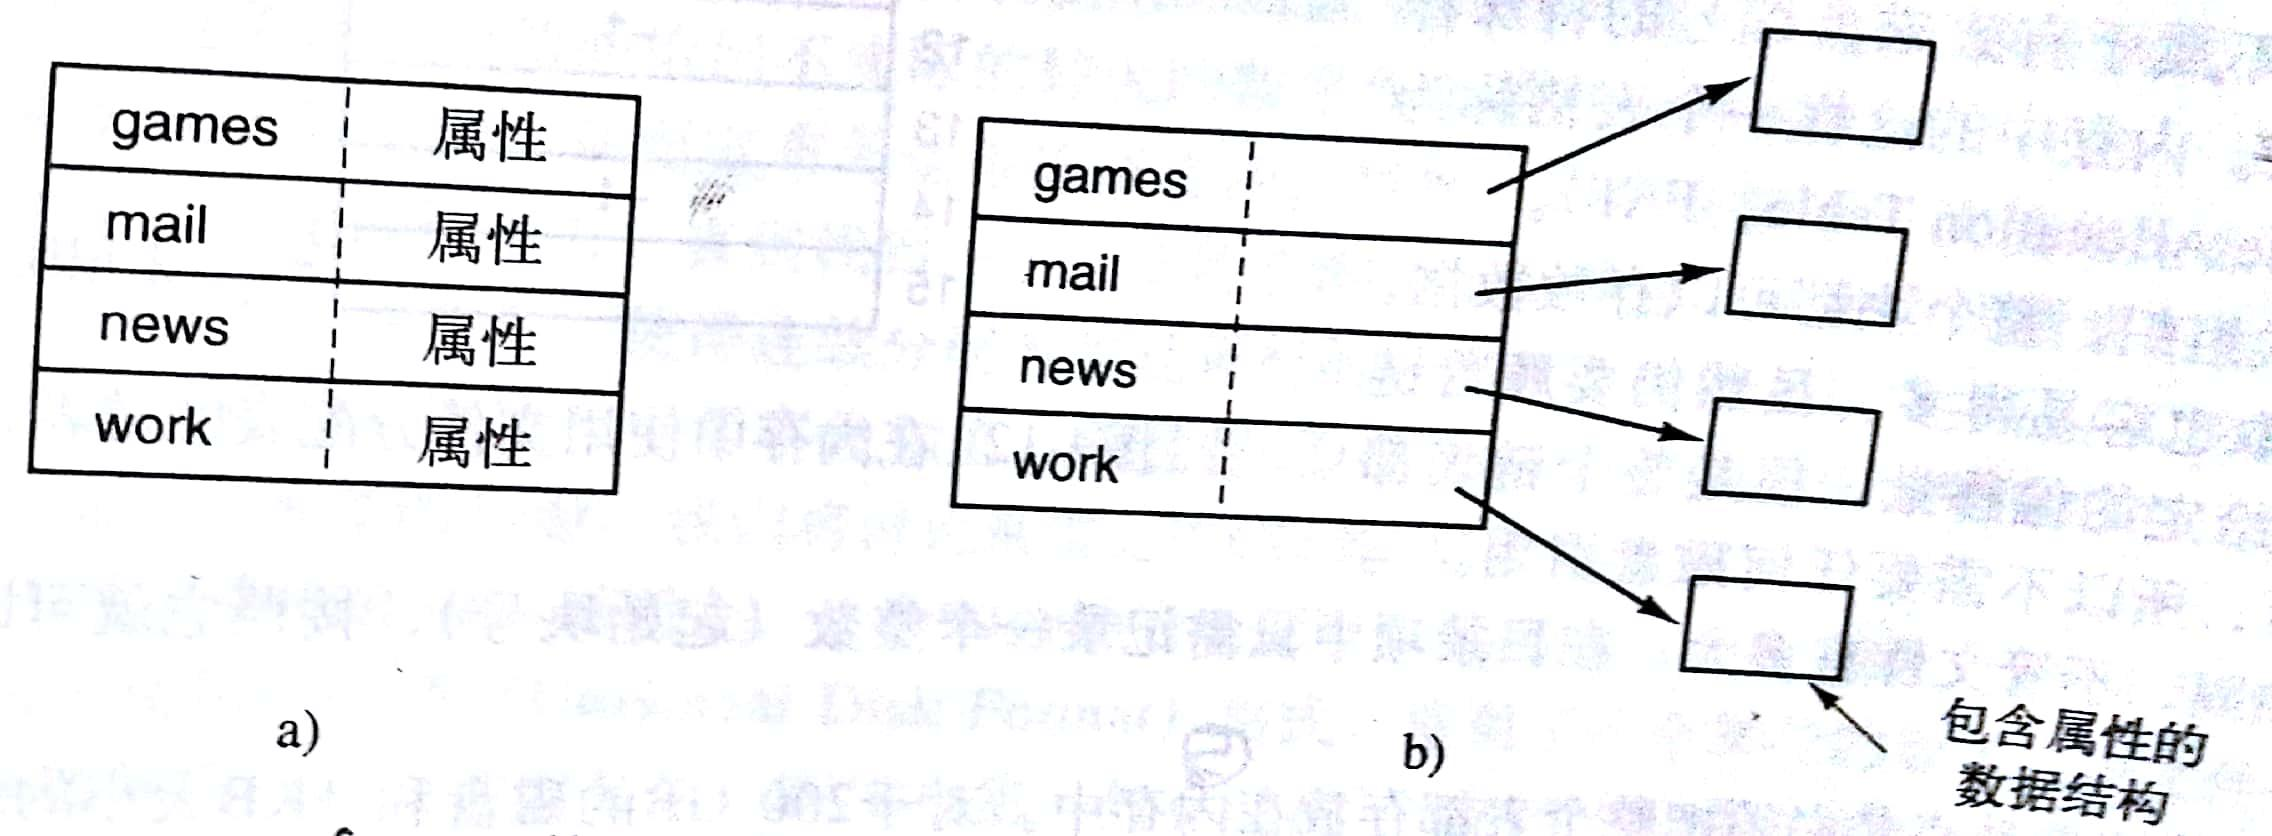
\includegraphics[scale = 0.15]{assets/ModernOperatingSystems/2018-01-08-16-09-39.png}
	\caption{a) 简单目录 , 包括固定大小的目录项,在目录项中有磁盘地址和属性 b)每个目录项只引用i节点的目录}
\end{figure}

\paragraph{如何实现可变长的文件名}
\begin{itemize}
	\item 限制文件名长度  , 典型值为 255个字节 , 但是这样会浪费了大量的目录空间, 因为只有很少文件会有这样长的名字
	\item 使目录自身都有固定的长度 , 而将文件名放置在目录后面的堆中
\end{itemize}

\paragraph{怎么在目录中定位文件?}
\begin{itemize}
	\item 使用线性查找的话 , 速度太慢, 一个加速的方法是 在每个目录中使用散列表
	\item 查找文件按照相同的过程进行 , 散列处理文件名字, 以便选择一个散列表项
	\item 使用散列表的优点是查找快速 , 缺点是需要复杂的管理 ;\\
	      只有在预计系统中的目录 经常会有成千上百个文件时 , 才把散列方案真正作为备用方案考虑
\end{itemize}

\subsubsection{共享文件}
\begin{figure}[H]
	\centering
	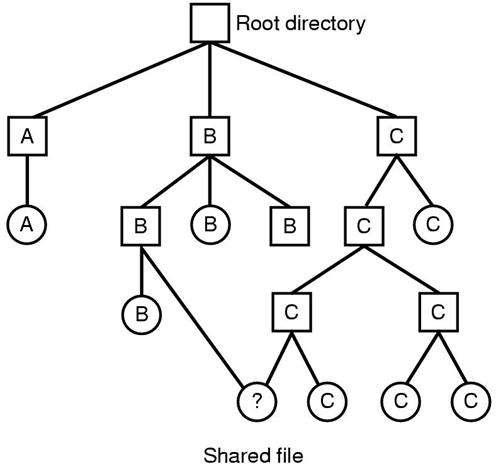
\includegraphics[scale = 0.5]{assets/ModernOperatingSystems/2018-01-08-16-34-09.png}
	\caption{有共享文件的文件系统}
\end{figure}

\paragraph{目录项不能含磁盘地址}  如果用户往文件中添加东西, 如果目录项是直接的磁盘地址 ,那么这次修改只会更新这个用户目录项 ,而其他用户对此一无所知,有两个解决方案(硬连接与符号连接的区别)
\begin{itemize}
	\item 列入一个与文件 本身关联的小型数据结构 , 目录将指向这个数据结构 , 而不是引用文件的地址 (UNIX中,这个数据结构是i节点)\\
	      i节点设置一个计数器 , 表示引用个数 ,只有i节点的计数为0  ,才最终删除这个文件
	\item 让系统建立一个新类型为 \textbf{LINK}的文件 , 并把该文件放在用户B的目录下 ,使得用户B与C的一个文件存在连接 \\
	      符号连接的实现需要额外的开销 , 但是只要简单的听一个机器的网络地址和文件路径, 就连接链接全球任何地方的机器上的文件
\end{itemize}

\subsubsection{日志结构文件系统 LFS Log-structured File System}
\paragraph{动机}  未来多数的磁盘访问时写操作 , 而零碎的磁盘操作是极其没有效率的

\paragraph{基本思想} 将整个磁盘机构化为一个日志 , 日志每一段的内容可能包含i节点 , 目录块等

\begin{itemize}
	\item 为了能找到i节点 ,必须维护一个由i节点编号索引组成的i节点图
	\item 所有的写操作都缓存在内存中 , 然后周期地把所有以缓存的写作为一个段 ,在日志文件末尾处写入磁盘
	\item LFS有一个清理线程 , 该线程周期地扫描日志进行磁盘压缩
\end{itemize}

\subsubsection{日志文件系统 Journaling File Systems}

\paragraph{动机及内容} : 虽然基于日志结构的文件系统是一个很吸引人的想法, 但是由于它们和现有的文件系统不相匹配,所以没有被广泛使用 。 但是其他文件系统也借鉴的日志的思想 : 保存一个用于记录系统下一步将要做什么的日志 ; 这样的文件系统 , 称为 \textbf{日志文件系统}

\paragraph{UNIX 移除文件的三个步骤} : 在目录中删除文件 , 释放i节点到空闲i节点池 ,将所有磁盘块归还空闲磁盘块池


\subsubsection{虚拟文件系统 VFS}
多种文件系统整合到一个统一的结构中 , 抽象出所有文件系统共有的部分 ,并且将这部分代码放在单独的一层 , 该层调用底层的时机文件系统来具体管理数据。

\begin{figure}[H]
	\centering
	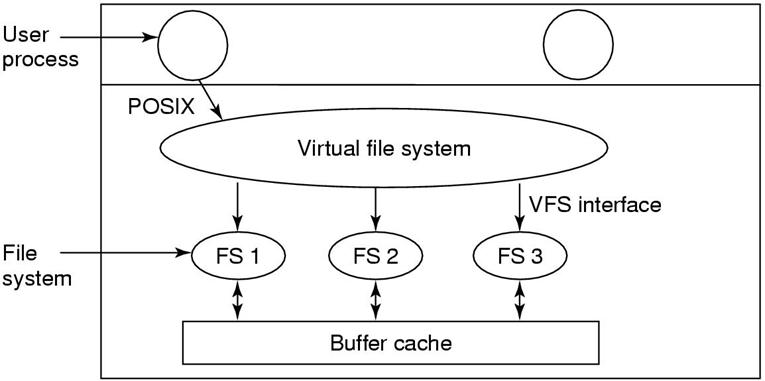
\includegraphics[scale = 0.5]{assets/ModernOperatingSystems/2018-01-08-16-50-41.png}
	\caption{虚拟文件系统的位置}
\end{figure}

\subsection{磁盘空间管理}
\subsubsection{磁盘块大小}
存储n个字节, 有两种分配策略 :分配连续的n个字节 , 或者把文件分成多个连续的块(逻辑连续 , 物理上不一定连续)

显然后者更灵活 , 但需要考虑一个因素 , 就是块的大小
\begin{itemize}
	\item 大的块, 对于小的文件浪费了大量的磁盘空间
	\item 小的块 ,意味着大多数文件会跨越多个块 , 因此需要多次寻到和旋转延迟才能读取它们,从而降低性能\footnote{读取时间 = 寻到时间 + 旋转延迟 + 传送时间}
\end{itemize}

\subsubsection{记录空闲块大小}
有两种策略:
\begin{itemize}
	\item 采用磁盘块链表 , 每个块包含尽可能多的空闲磁盘块号(其中一个位置用来存放指向下一块的指正)
	\item 位图管理 , n个块的磁盘需要n位 , 用1表示空闲 , 用0表示已分配(或者反之)
\end{itemize}


内存中有一个指针块用来保存一个磁盘块, 在使用的时候, 直接读内存即可 ,  但当这个指针块快满 或者很少的时候 , 可能还是会产生一次不必要的I/O  : 申请空闲块不够 , 或者释放空闲块的时候 ,不够位置存放指针 ,这就将要导致一次I/O操作

优化 : 保持磁盘上大多数磁盘块为满的状态(减少磁盘的使用) , 但是在内存中 保留一个半满的指针块, 这样它可以既处理文件的创建又处理文件的删除操作 , 而不会为空闲表进行磁盘I/O

\begin{figure}[H]
	\centering
	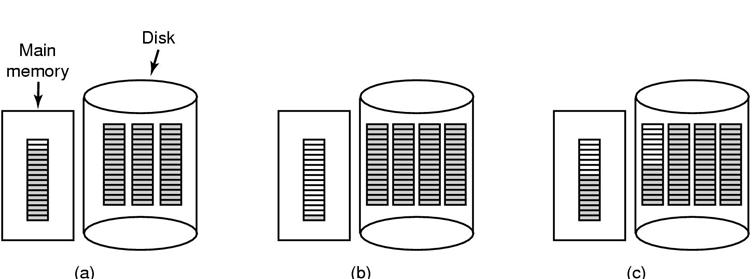
\includegraphics[scale = 0.5]{assets/ModernOperatingSystems/2018-01-08-19-00-19.png}
	\caption{1) 在内存中一个被指向空闲磁盘块的指针几乎满的块 ,以及磁盘上的3个指针块  ;b) 释放一个有3个块的文件结果 ; c)处理该3个块的替换策略(待阴影的表项代表指向空闲磁盘块的指针)}
\end{figure}

\subsubsection{磁盘配额}
\begin{figure}[H]
	\centering
	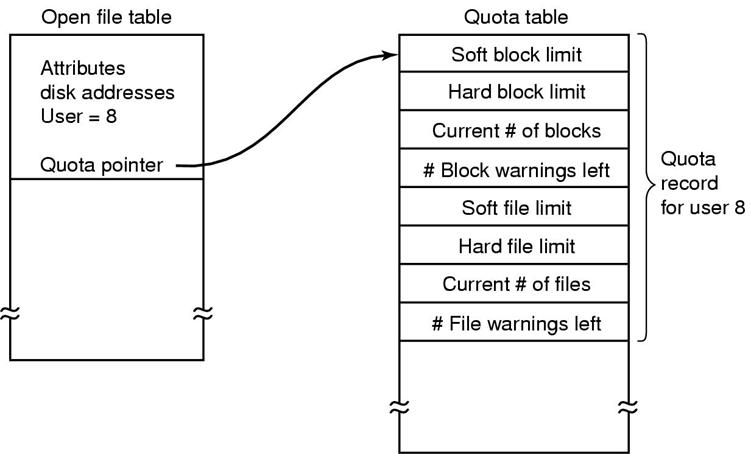
\includegraphics[scale = 0.5]{assets/ModernOperatingSystems/2018-01-08-19-02-57.png}
	\caption{在配额表中记录了每个用户的配额}
\end{figure}


\subsubsection{文件系统备份}
\paragraph{备份的两个原因}
\begin{itemize}
	\item 从意外的灾难中恢复
	\item 从错误的操作中恢复
\end{itemize}

\paragraph{备份需要考虑的5个问题}:
\begin{itemize}
	\item 备份的内容 : 是备份这个文件系统,还是备份一部分 , 系统文件是没必要备份的
	\item 是否是增量备份 : 全量备份意味着更多的空间消耗
	\item 是否需要对备份文件进行压缩 : 压缩文件部分损坏, 将导致整个备份不可用
	\item 备份的时间 : 对活动文件备份是很难的 , 可以选择脱机备份 , 也可以选择快照
	\item 备份设备的存放 : 备份应该远离现场存放
\end{itemize}


\paragraph{转储磁盘到磁带的两种方案:}
\begin{itemize}
	\item 物理转储 : 从磁盘的第0块开始 , 将全部块按序输出到磁带上 , 直到最后一块复制完毕
	\item 逻辑转储 : 从一个或指定几个目录开始 , 递归地转储其自给定基准日期后所更改的全部文件和目录
\end{itemize}

\begin{figure}[H]
	\centering
	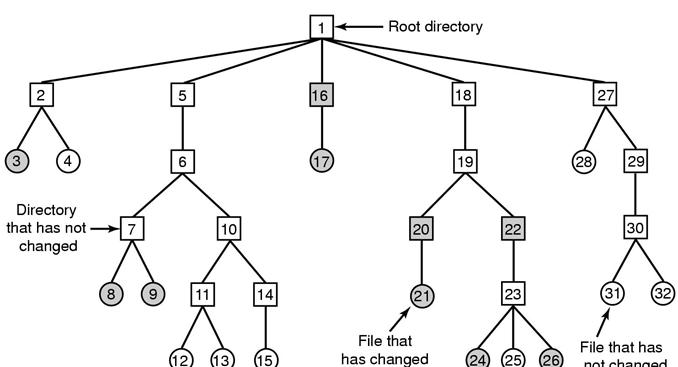
\includegraphics[scale = 0.6]{assets/ModernOperatingSystems/2018-01-08-19-18-20.png}
	\caption{待转储的文件系统 , 方框代表目录 , 圆圈代表文件 , 被阴影覆盖的表示自上次转储以来修改过的,每个目录和文件都被标上其i节点号}
\end{figure}

\paragraph{维护一个以i节点号为索引的位图}:
\begin{figure}[H]
	\centering
	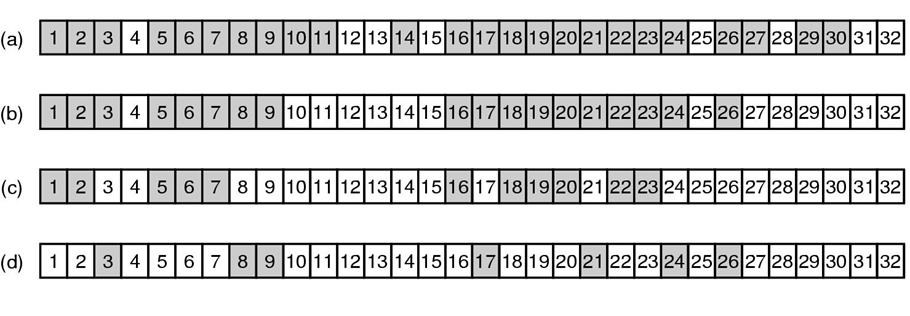
\includegraphics[scale = 0.6]{assets/ModernOperatingSystems/2018-01-08-19-21-56.png}
	\caption{$a$: 所有修改过的文件 和 全部目录 ; $a\to b$ : 去掉未被修改也未被引用的目录 , 这里引用的意思是 以5和6为例,8,9所对应的目录虽然没有被修改 , 但是恢复8,9需要用到它们,因此也要保存5,6两个目录的i节点 ;$c$待转储的目录 , $d$待转储的文件}
\end{figure}

\subsubsection{文件系统一致性}
\paragraph{一致性检查分为两种}
\begin{itemize}
	\item 块的一致性检查
	\item 文件的一致性检查
\end{itemize}

\paragraph{块检查方法}:设立两个表 ,一个表记录每个空闲块的索引次数, 一个表记录每个非空闲块的索引数目

\begin{figure}[H]
	\centering
	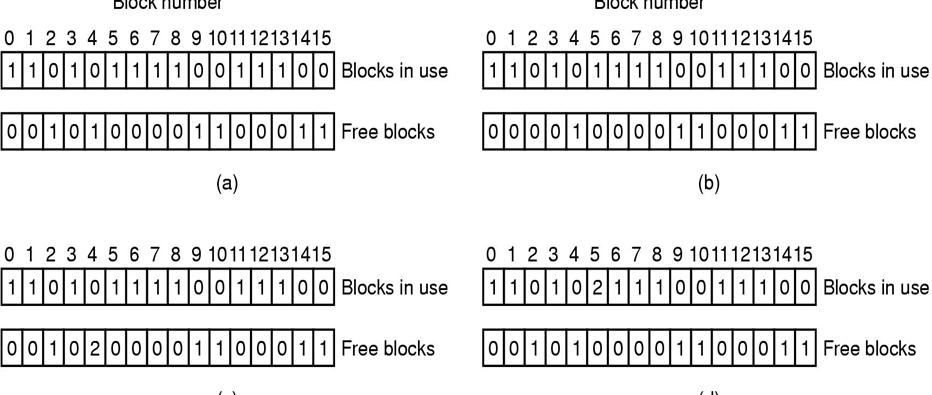
\includegraphics[scale = 0.5]{assets/ModernOperatingSystems/2018-01-08-19-30-43.png}
	\caption{文件系统状态 : a) 一致  ;b) 块丢失 ; c) 空闲表有重复快 ; d)重复数据块}
\end{figure}

\begin{itemize}
	\item 当每个块 或者在一个表中为1 , 或者在第二个表中为1, 则表示一致
	\item 块丢失 : 存在一个块 不出现在两个表中 ; 把块加入到空闲表中
	\item 空闲表重复 : 块在空闲表中出现了多次 ; 重建空闲表
	\item 数据块重复 : 多个文件使用同一块磁盘块 , 把重复的块复制到空闲块,并把该块插入到其中一个文件 以保持一致性 (虽然可以确定块的内容是不对的,但是这个后果由用户承担)
\end{itemize}

\subsection{文件系统性能}
\begin{itemize}
	\item 高速缓存
	\item 块提前读 : 在用到块之前,试图提前将其写入高速缓存 , 以提高命中率
	\item 减少磁盘臂运动
	      \begin{itemize}
		      \item i节点放在磁盘中部而不是开始 , 此时 i节点和第一块之间的平均寻道时间为原来一半;
		      \item 将磁盘划分成多个柱面组, 每个柱面组有自己的i节点、数据块、空闲表
	      \end{itemize}
\end{itemize}

\subsection{文件系统实例}
\paragraph{文件系统实例} : CD-ROM文件系统 , MS-DOS文件系统 , UNIX V7文件系统

\paragraph{UNIX V7}
\begin{figure}[H]
	\centering
	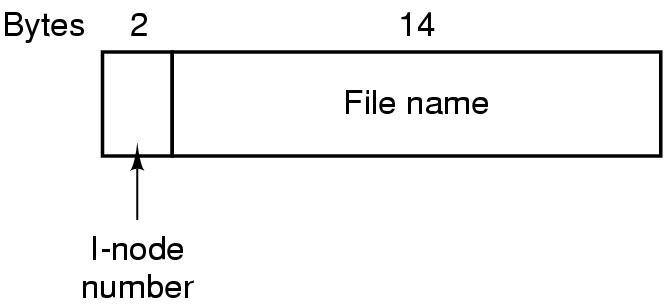
\includegraphics[scale = 0.3]{assets/ModernOperatingSystems/2018-01-08-19-49-10.png}
	\caption{UNIX V7的目录表项}
\end{figure}

\begin{figure}[H]
	\centering
	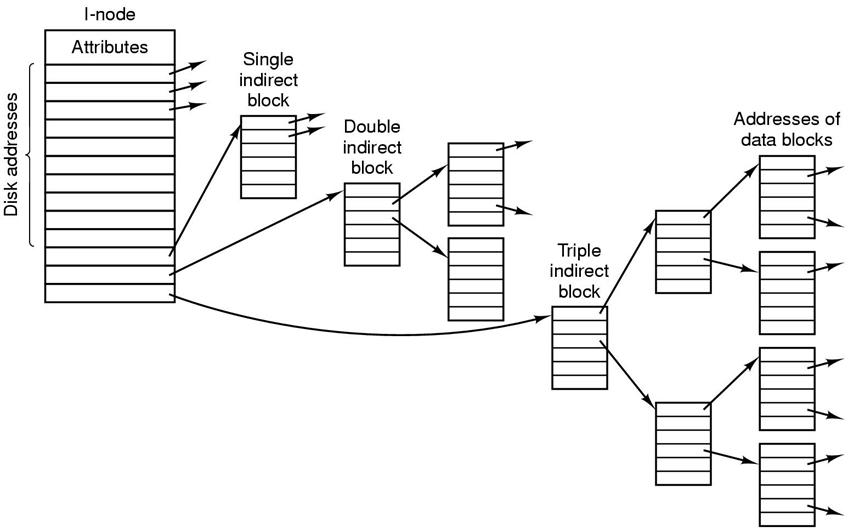
\includegraphics[scale = 0.6]{assets/ModernOperatingSystems/2018-01-08-19-49-31.png}
	\caption{一个UNIX的i节点 , 一个为一次间接块 ,一个为2次间接块 ,一个为三次间接块, 其余为i节点}
\end{figure}

\begin{figure}[H]
	\centering
	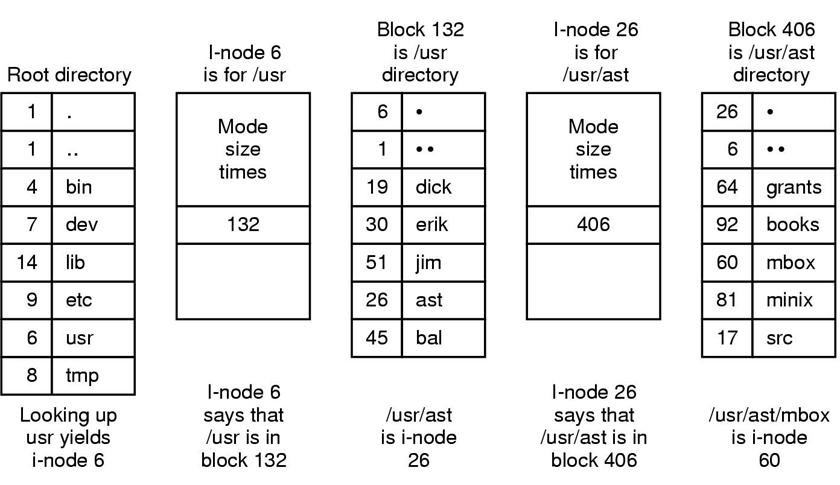
\includegraphics[scale = 0.6]{assets/ModernOperatingSystems/2018-01-08-19-50-18.png}
	\caption{查找/usr/ast/mbox的过程 , \textbf{根目录的$..$指向自己}}
\end{figure}

\section{输出 / 输出}
\subsection{I/O 硬件原理}
\subsubsection{I/O设备分类}
I/O设备分类:
\begin{itemize}
	\item 块设备 : 把信息存储到特定的块中,每个块有自己的地址 , 且独立其他块而读写\\
	通常块大小为512字节-32768字节 \\
	常见的块设备有:硬盘 、 CD-ROM 、 USB盘
	\item 字符设备 : 以字符为单位发送或接收字符流 , 而不考虑任何块结构 , 不可寻址 , 也没有任何寻到操作
	\\常见的字符设备有 : 打印机 、 网络接口 、 鼠标 以及大多数与磁盘不同的设备
	\item 其他 : 有些设备既不是块设备 , 也不是字符设备
	\subparagraph{时钟} 时钟既不是块可寻址的 , 也不产生或接收字符流 ;它所做的工作就是按照预先规定好的时间间隔产生中断
	\subparagraph{内存映射的显示器}
\end{itemize}

\subsubsection{I/O设备组成} 
I/O设备组成: \textbf{机器部件} 和 \textbf{电子部件} 两个部分
\begin{itemize}
	\item 机器部件 : 机器部件就是设备本身
	\item 电子部件 : 又称 设备控制器 、适配器 \\
	在计算机中通常以主板上的芯片 或者 插入扩展槽中的印刷电路板的形式出现
	\subparagraph{适配器的任务} 把串行的位流转换成字节块, 并进行必要的错误校正工作 : 字节块通常首先在控制器内部的一个缓冲区进行组装 , 然后在对校验和进行检验并证明块没有错误后 , 再将它复制到主存中
\end{itemize}
\begin{figure}[H]
	\centering
	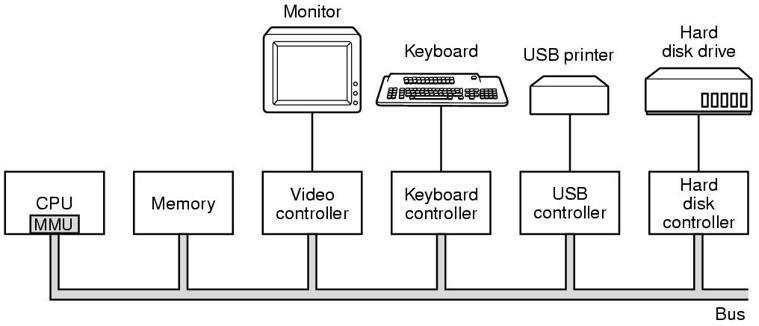
\includegraphics[scale = 0.3]{assets/ModernOperatingSystems/2018-01-10-15-14-47.png}
	\caption{设备的机器部件 与 适配器}
\end{figure}

\subsubsection{内存映射 I / O}
\paragraph{CPU如何与设备的控制寄存器和数据缓冲区进行通信 ? }
\begin{itemize}
	\item 每个控制寄存器被分配一个 I/O 端口号 (I/O port , 8位或16位的整数) ,所有I/O端口形成 I/O空间 , 普通用户程序不能对其进行访问(只有操作系统可以访问 , 使用特殊的I/O指令)
	\item 将所有控制寄存器映射到内存空间中 , 这样的系统被称为 \textbf{内存映射 I/O}
	\item 混合上面两种
\end{itemize}

\paragraph{内存映射 I/O优缺点}
\begin{itemize}
	\item 对内存映射I/O, I/O设备驱动可以完全用C语言编写,因为设备控制寄存器只是内存中的变量;如果不使用内存映射I/O,要用到汇编代码
	\item 对内存映射I/O,不需要特殊的保护机制来阻止用户进程执行I/O操作
	\item 可以引用内存的每一条指令也可以引用控制寄存器;如果不使用内存映射I/O,必须首先将控制寄存器读入CPU  , 然后再检测 , 这就需要两条指令而不是一条
	\item 对内存映射I/O,硬件必须针对每个页面具备选择性禁止高速缓存的能力。否则可能出现一直读取缓存中过期的值导致进入死循环
\end{itemize}

\subsubsection{直接存储器存取 DMA}
\paragraph{动机} : CPU可以从I/O控制器每次请求一个字节的数据, 但是这样做会浪费cpu时间 , 所以 使用 \textbf{DMA}代替 CPU进行磁盘的I/O操作 , 它总能独立于CPU而访问系统总线

\paragraph{DMA的组成} DMA包含若干个可以被CPU读写的寄存器 , 其中包括一个内存地址寄存器 、字节计数器 和一个或多个控制存储器 

控制存储器指定要使用的I/O端口 、传送方向(从I/O设备读或者写) 、 传送单位(每次一个字节或一个字) 以及在突发的传输中要传送的字节数

\begin{figure}[H]
	\centering
	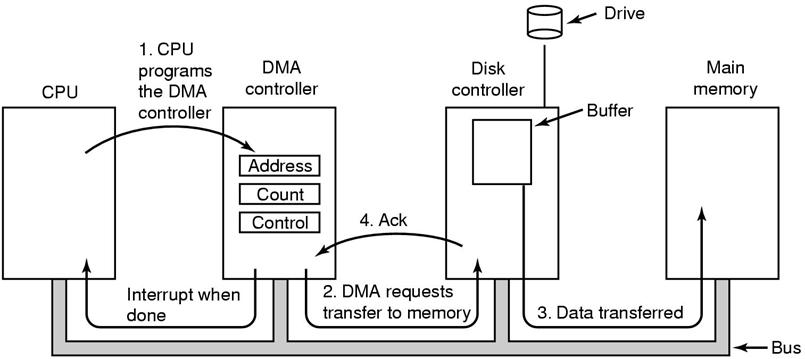
\includegraphics[scale = 0.5]{assets/ModernOperatingSystems/2018-01-10-16-05-53.png}
	\caption{DMA传输的4个步骤}
\end{figure}

\subsubsection{中断}
当一个I/O设备完成交给它的工作时 , 它就产生一个中断 (假设系统已经开放中断) , 它是通过在分配给它的一条 \textbf{总线信号线} 上置起信号而产生中断的 ,该信号被主板上的中断控制器芯片检测到 ,由中断控制芯片决定做什么

\begin{figure}[H]
	\centering
	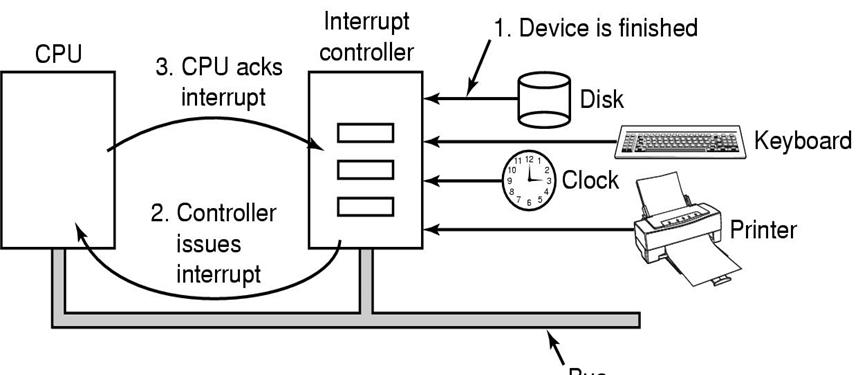
\includegraphics[scale = 0.5]{assets/ModernOperatingSystems/2018-01-10-16-10-14.png}
	\caption{中断产生的过程}
\end{figure}

\paragraph{在何处保存状态信息?}
\begin{itemize}
	\item 专用的寄存器 
	\item 用户的堆栈
	\item 内核堆栈
\end{itemize}

\paragraph{精确中断和不精确中断}
\begin{figure}[H]
	\centering
	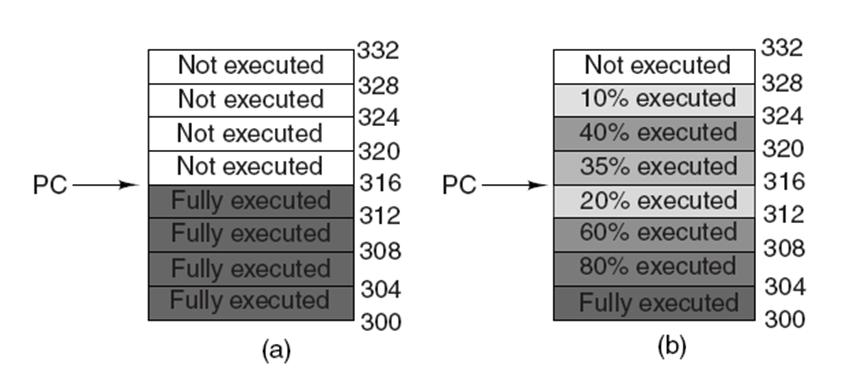
\includegraphics[scale = 0.5]{assets/ModernOperatingSystems/2018-01-10-16-14-02.png}
	\caption{a)精确中断 b)不精确中断}
\end{figure}

在超标量的CPU中 , 当发生中断的时候 , 可能有多个指令处于执行状态 , 并且完成的程度个不相同 , 那么处理这些中断就需要保存大量的信息(多条指令) , 而恢复的时候也是 , 从而造成了中断响应和恢复十分缓慢

\subsection{I/O 软件原理}

\subsubsection{I/O软件的目标}
\paragraph{6个I/O软件的目标} 
\begin{itemize}
	\item 设备独立性 : I/O软件能访问任意的I/O设备而无需实现指定设备
	\item 统一命名 : 一个文件或一个设备的名字应该是一个简单的字符串或一个整数
	\item 错误处理 : 只有在底层软件处理不了的情况下,才将错误上交给高层处理
	\item 同步(阻塞)和异步(中断驱动)传输 
	\item 缓冲 : 数据离开一个设备之后通常并不能直接存放到其最终的目的地\\
	某些设备具有严格的实时约束(数字音频设备) , 所以设备必须预先放置到输出缓冲区之中, 从而消除缓缓冲区填满和缓冲区清空速率之间的相互影响, 以避免缓冲区欠载
	\item 共享设备和独占设备 : 操作系统必须能够处理共享设备和独占设备以避免问题发生
\end{itemize}

\subsubsection{I/O的方式}
\paragraph{3种I/O方式}
\begin{itemize}
	\item 程序控制 I/ O :让CPU做全部工作
	\item 中断驱动 I/O  : 使CPU不再忙等设备 而是转去处理其他事 , 当设备就绪 , 产生中断再进行后续操作
	\item DMA : 使用DMA代替CPU控制I/O , 当缓冲区传输完成才产生中断
\end{itemize}

\subsection{I/O软件层次}
\paragraph{I/O软件的4个层次} :(低$\to$高) 设备中断处理程序 、设备驱动程序 、 与设备无关的I/O软件  、 用户级I/O软件

\begin{figure}[H]
	\centering
	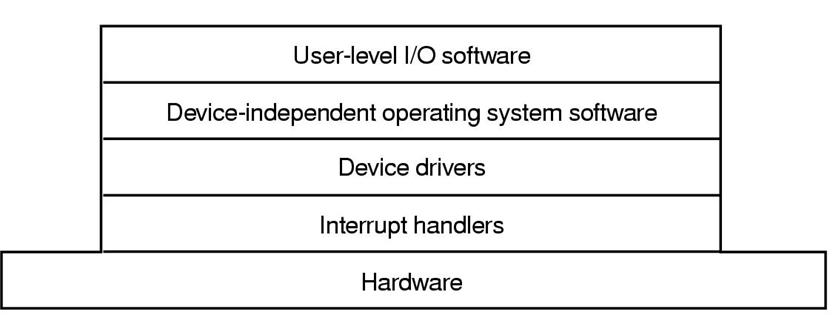
\includegraphics[scale = 0.5]{assets/ModernOperatingSystems/2018-01-10-16-32-15.png}
	\caption{I/O软件系统的层次}
\end{figure}

\paragraph{中断处理程序}
应该将中断处理程序隐藏在操作系统内部以便操作系统的其他部分不与他们发生联系 , 隐藏的办法是 :
启动一个I/O操作的驱动程序阻塞起来,直到I/O操作完成且产生一个中断。

当设备I/O完成之后 , CPU再对程序进行后续操作

\paragraph{设备驱动程序}
每个连接到计算机的I/O设备 ,都需要某些特定的代码来对其进行控制 , 这样的代码 称为 \textbf{设备驱动程序}

每个设备驱动程序通常处理一种类型的设备或者至多一类紧密相关的设备

\paragraph{设备驱动程序的一般功能} 接受请求、对设备进行初始化、管理电源需求和日志事件

\paragraph{设备驱动程序一般结构}
\begin{itemize}
	\item 启动时检查输入参数,如果有效,进行抽象到具体的转换
	\item 检查设备当前是否在使用:在使用,请求被排队;空闲,检查硬件状态了解请求是否能得到处理,可能的话,接通设备或启动马达,开始实际的控制(向设备发出一系列命令
\end{itemize}

\begin{figure}[H]
	\centering
	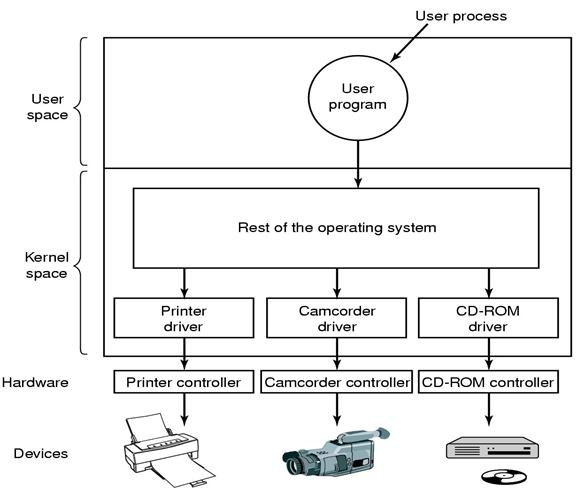
\includegraphics[scale = 0.5]{assets/ModernOperatingSystems/2018-01-10-16-59-35.png}
	\caption{设备驱动程序的逻辑定位}
\end{figure}

\paragraph{与设备无关的I/O软件的功能}
\begin{itemize}
	\item 设备驱动程序的同一接口
	\item 缓冲
	\item 错误报告
	\item 分配与释放专用设备
	\item 与设备无关的块大小
\end{itemize}

\paragraph{用户空间的I/O软件}包括与用户程序连接在一起的库(或Spooling系统)及完全运行与内核之外的程序.
\begin{itemize}	
	\item 库过程 : 系统调用通常由库过程实现。 C程序调用 count=write(fd,buffer,nbytes);
	\item 假脱机技术 : 并非所有的用户层I/O软件都是由库过程组成的,
另一个重要的类别是假脱机系统Spooling, Spooling是多道程序设计系统中处理独占I/O设备的一种方法。
\end{itemize}

\paragraph{小结} 

\begin{figure}[H]
	\centering
	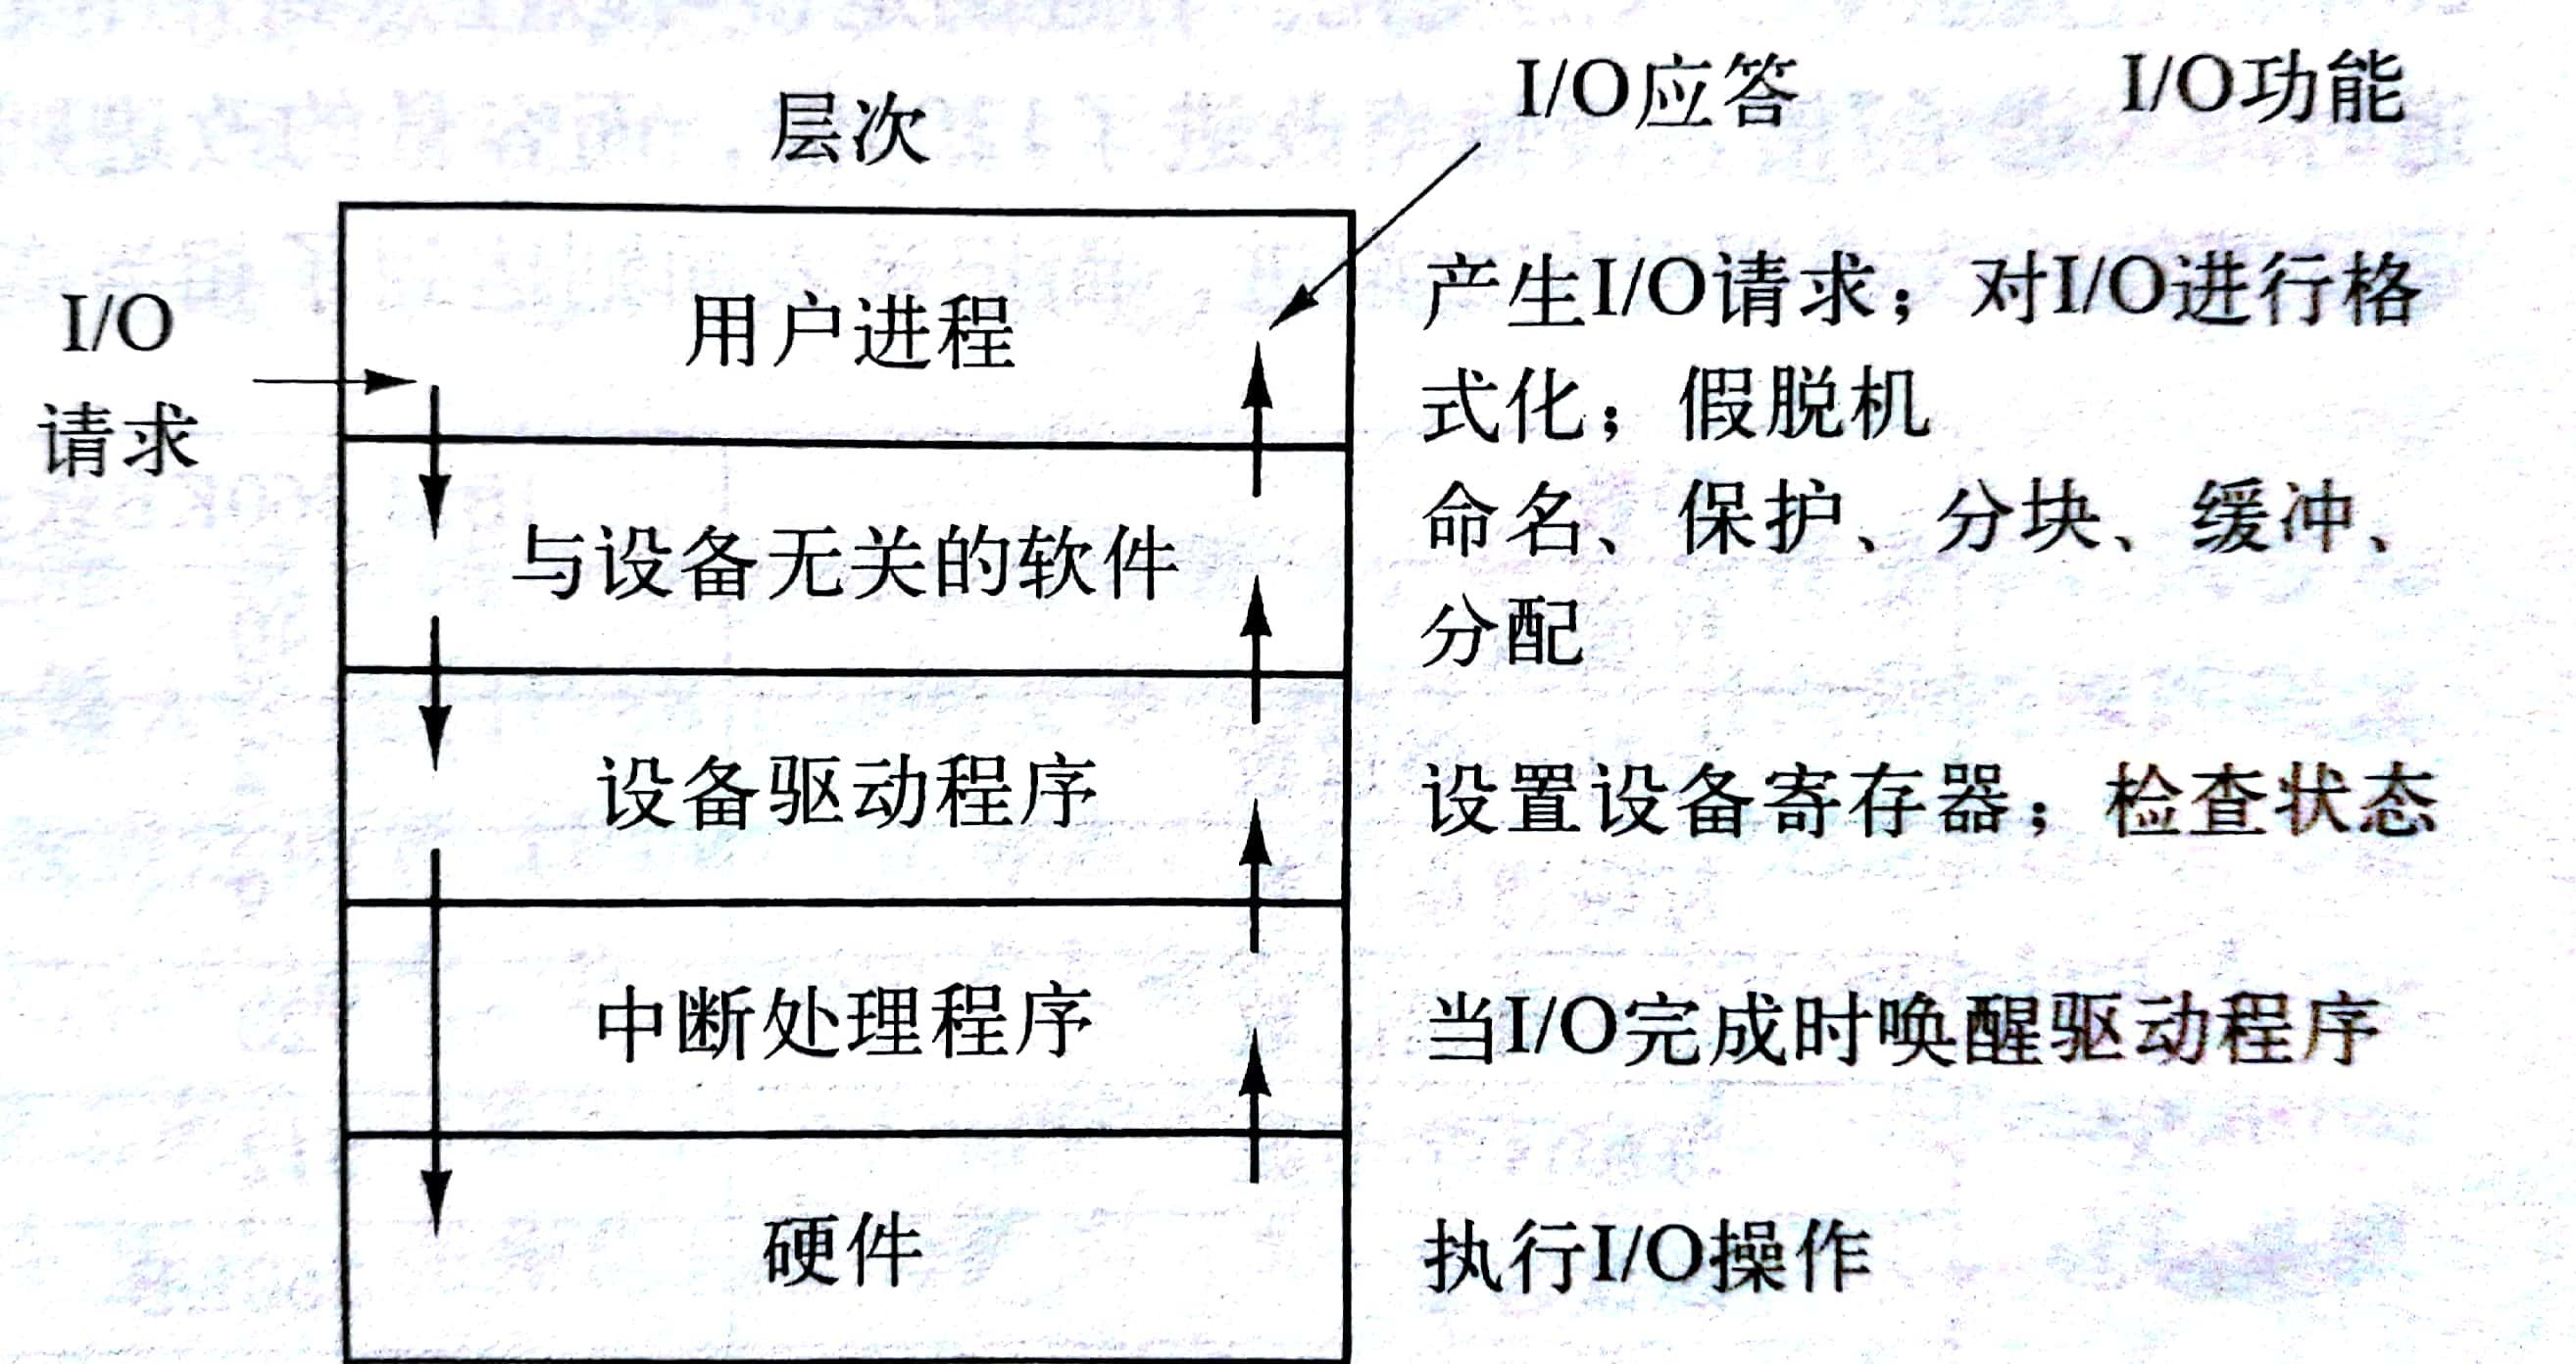
\includegraphics[scale = 0.1]{assets/ModernOperatingSystems/2018-01-10-17-11-23.png}
	\caption{I/O的层次以及每一层次的功能}
\end{figure}

\subsection{盘}
\subsubsection{磁盘}
喵喵喵

\subsubsection{RAID}
\paragraph{动机} CPU的性能一直呈指数指数增长 , 但是磁盘的性能却不是

\paragraph{诞生} Patterson等人1988 提出使用六种特殊的磁盘组织可能会改进磁盘的性能、可靠性或者两者同时改进 , 导致 RAID的诞生

初始 RAID指 廉价磁盘冗余阵列 Redundant Array of Inexpensive Disk  ,工业界将I重定义为 Independent

\paragraph{基本思想} 将一个装满了磁盘的盒子安装到计算机 , 用RAID控制器替换磁盘控制器卡, 将数据复制到整个RAID上 ,然后进行常规操作;对软件而言, 看起来就像磁盘一样 ; 

除此之外 , 所有的RAID都具有同样的特性, 那就是将数据分布在全部驱动器上 , 这样就可以进行并行操作

\paragraph{0-5级 6种 RAID}
\begin{itemize}
	\item 0级RAID : 将RAID模拟的虚拟单个磁盘划分成条带\footnote{像这样将数据分布在多个驱动器上称为划分条带} ,每个条带k个扇区, 以转轮的方式写到全部驱动器上
	\paragraph{控制器的责任} 分解请求 , 并且以正确的顺序将适当的命令提供给适当的磁盘,之后还要在内存中将结果正确地装配起来
	
	\item 1级RAID : 这是一个真正的RAID , 在0级RAID的基础上 , 它复制了所有磁盘 , 所以有主磁盘和副磁盘 ;执行写操作的时候被写两次, 执行读的时候读取任意一个副本都可以 ; 
	\\因此读性能是单个驱动器的两倍 ; 由于副本的原因 ,容错性能也是突出的

	\item 2级RAID : 以字或字节为单位 , 将字节拆开成多个部分 ,每个部分分别进行汉明编码, 将汉明编码分别写入每个磁盘中
	\item 3级RAID :是对2级RAID的简化 , 每个数据字计算一个奇偶校验位 , 并保存在一个奇偶驱动器中
	\item 4级RAID : 使用条带而不是奇偶校验一个字 , 将得到的奇偶条带写到额外的磁盘上
	\item 5级RAID : 4级RAID中, 奇偶驱动器可能成为瓶颈 , 因此 , 5级RAID通过循环的方式在所有的驱动器上均匀地分布奇偶校验位
\end{itemize}

\begin{figure}[H]
	\centering
	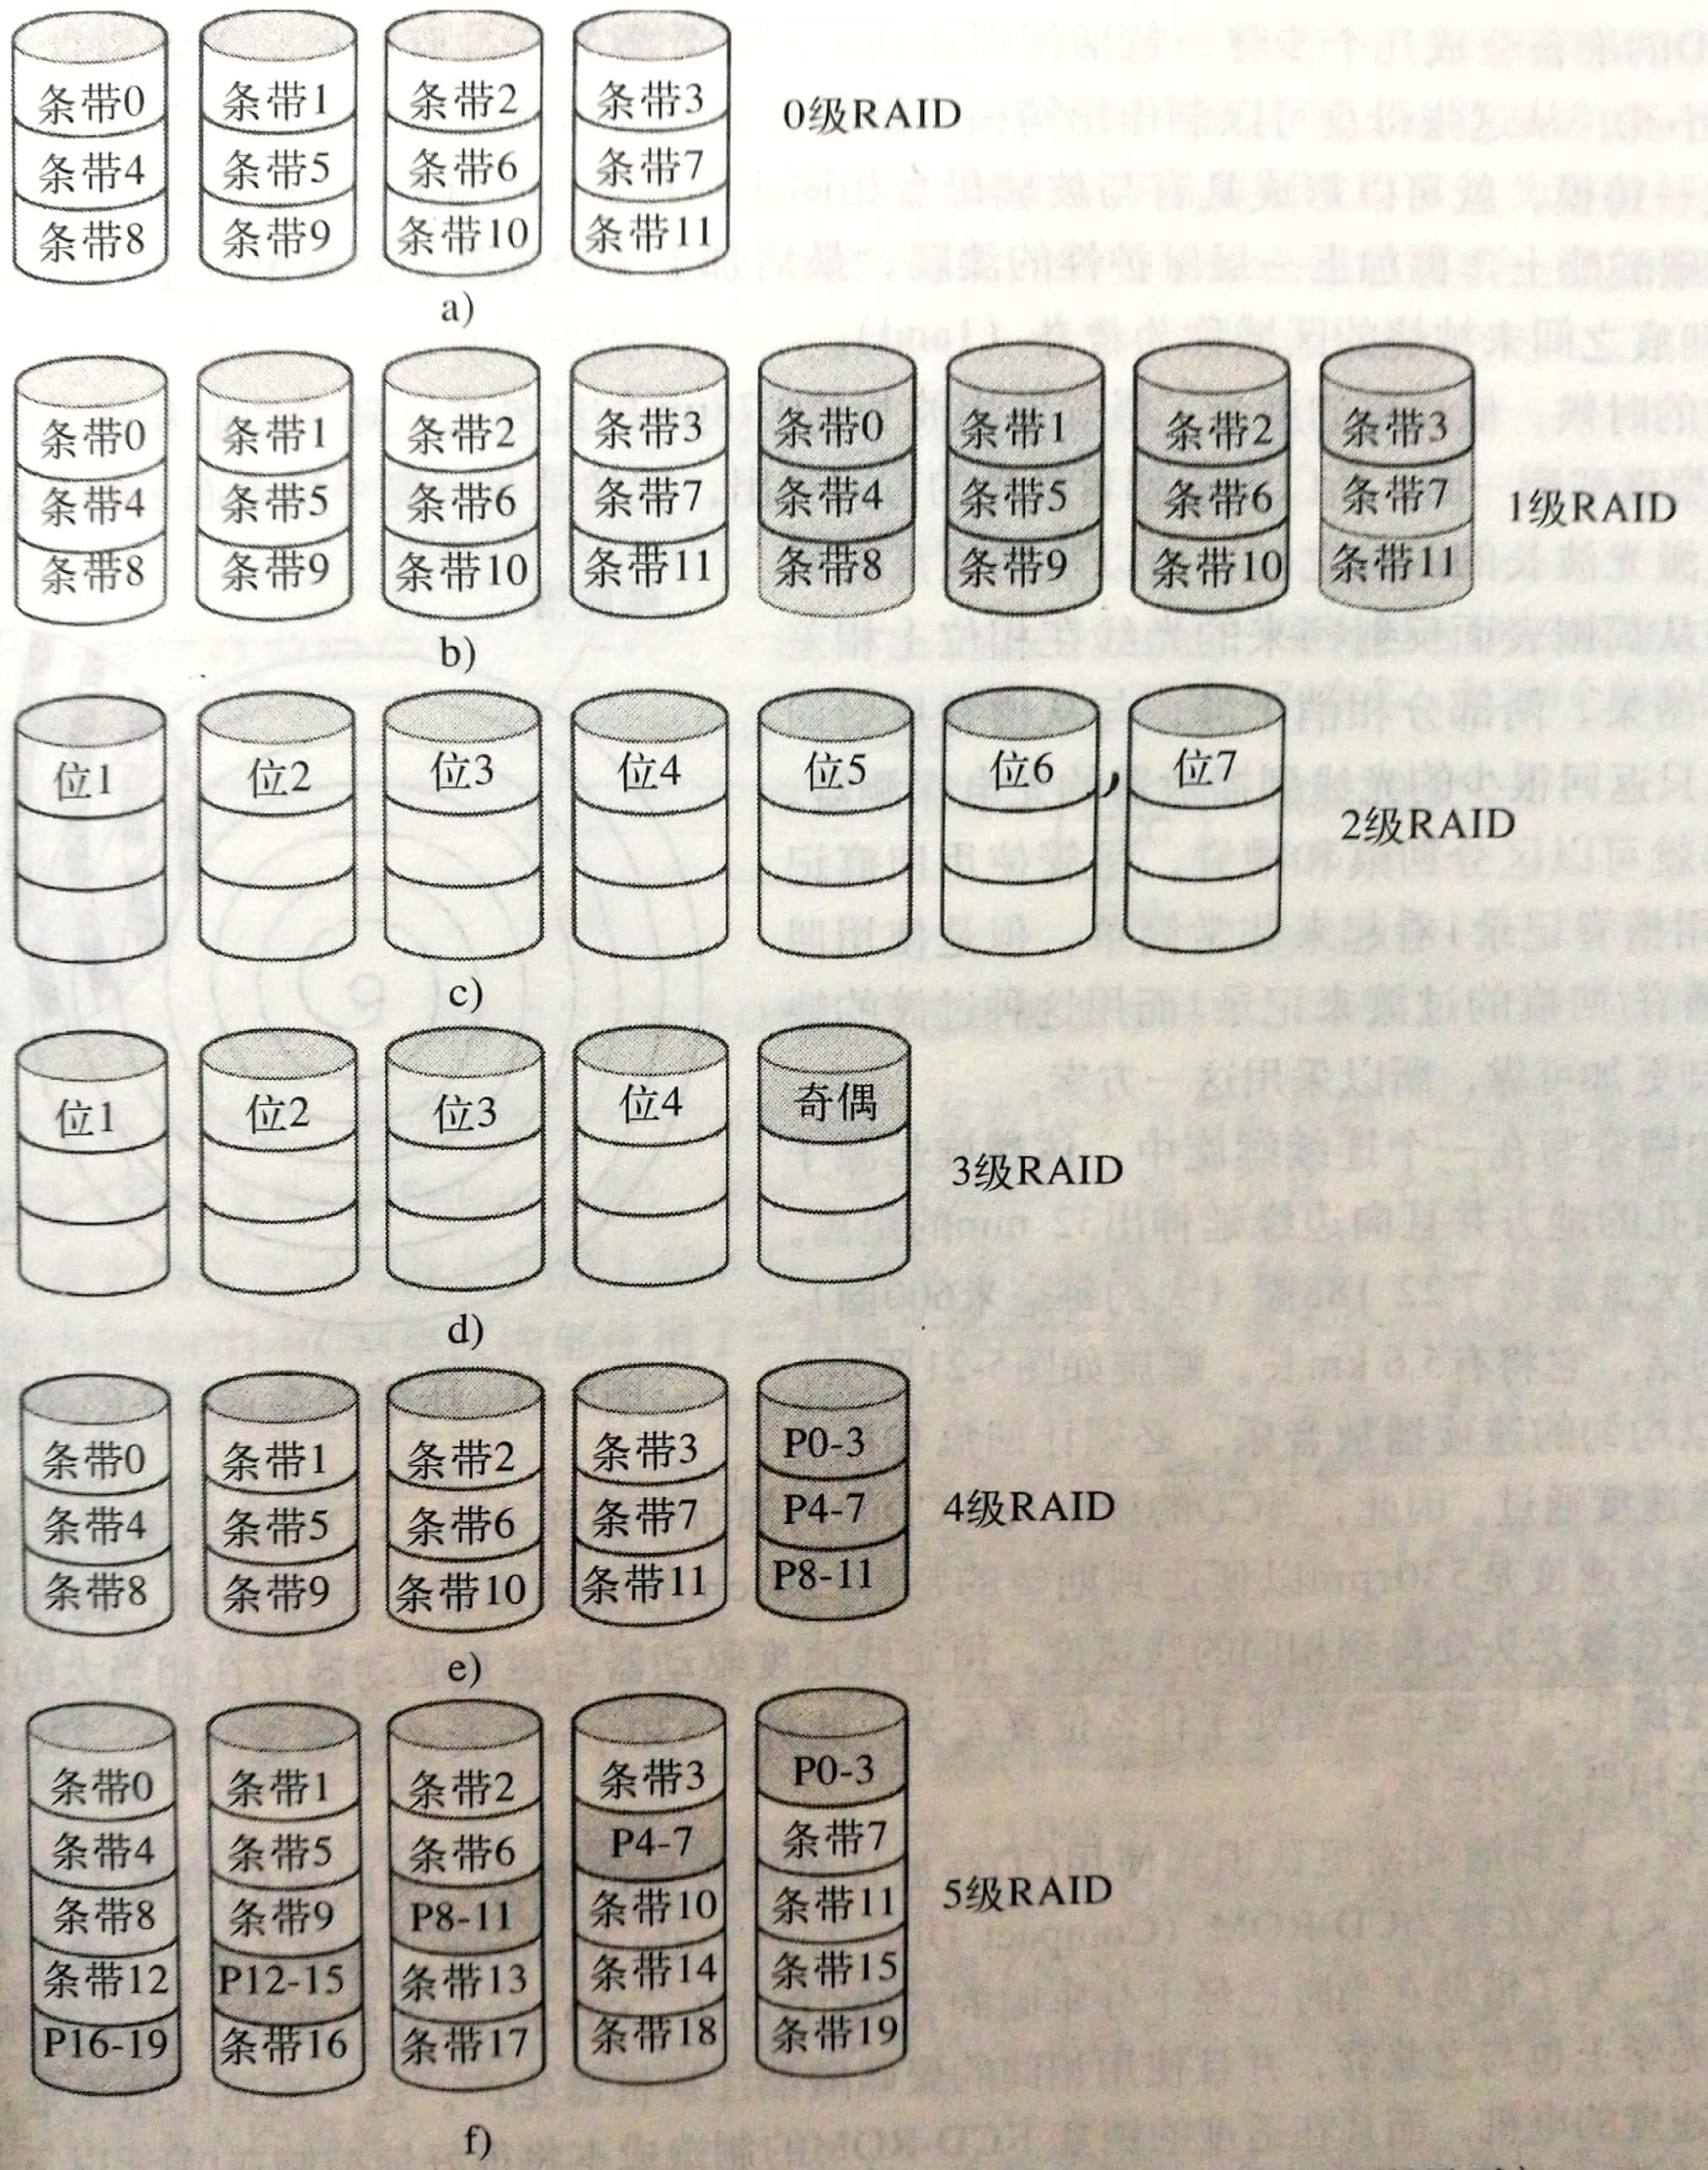
\includegraphics[scale = 0.3]{assets/ModernOperatingSystems/2018-01-10-17-53-40.png}
	\caption{0级RAID到5级RAID(备份驱动器及奇偶驱动器以阴影显示)}
\end{figure}

\subsubsection{CD-ROM}
喵喵喵

\subsection{磁盘格式化}
低级格式化的结果是磁盘容量减少 , 减少的量取决于前导码 、扇区间间隙 和ECC的大小以及保留的备份扇区的数目

\footnote{\color{red}只有在关于内存和磁盘大小的情况下 ,K , M , 等才取为2的幂}


\subsubsection{磁盘臂调度算法}
\paragraph{磁盘块读写时间的3个因素}
\begin{itemize}
	\item 寻道时间 : 将磁盘臂移动到适当的柱面所需时间
	\item 旋转延迟 : 等待适当扇区旋转到磁头下所需的时间
	\item 实际数据传输时间 : 实际数据传输时间
\end{itemize}

\paragraph{3种磁盘臂调度算法}
\begin{itemize}
	\item 先来先服务 FCFS 
	\item 最短寻道优先 SSF : 总是处理与磁头距离最近的请求以使寻到时间最小化
	\begin{figure}[H]
		\centering
		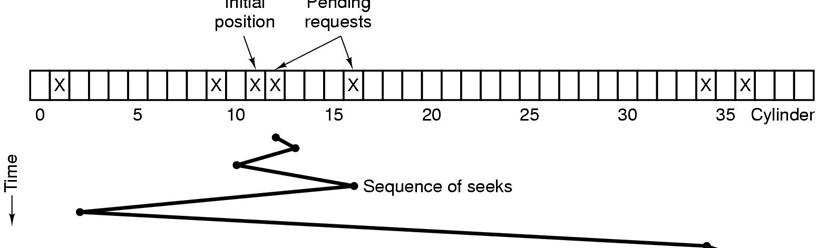
\includegraphics[scale = 0.5]{assets/ModernOperatingSystems/2018-01-10-18-04-58.png}
		\caption{初始位置为11 , 如请求为:1,36,16,34,9,12.(FCFS顺序)
SSF访问顺序为12,9,16,1,34,36。
Shortest Seek First (SSF) disk scheduling algorithm
移动磁道数为1,3,7,15,33,2,共61个柱面}
	\end{figure}
	
	\item 电梯算法 : 又称扫描算法 SCAN : 按一个方向移动 , 直到在那个反向上没有请求为止 , 然后改变方向\\
	电梯算法对任一一组给定的请求 , 磁盘臂移动总次数的上界是固定的,正好是柱面数的两倍

	\begin{figure}[H]
		\centering
		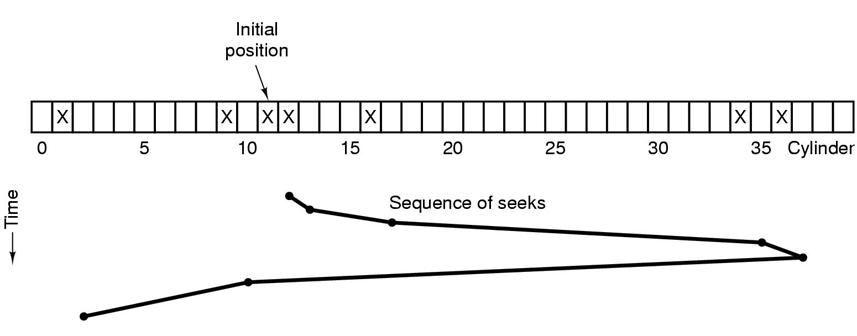
\includegraphics[scale = 0.5]{assets/ModernOperatingSystems/2018-01-10-18-05-23.png}
		\caption{访问顺序为 12,16,34,36,9,1 ; 
The elevator algorithm(电梯算法) for scheduling disk requests
移动磁道数为1,4,18,2,27,8,共60个柱面}
	\end{figure}
	
\end{itemize}

\subsubsection{错误处理}

\paragraph{坏扇区的两种处理方法}控制器处理或操作系统处理
\begin{itemize}
	\item 控制器处理 : 将坏扇区列表写在磁盘, 对于每个磁盘, 使用一个备用扇区替换它
	\begin{itemize}
		\item 将备用扇区映射为错误扇区
		\item 将所有扇区向后移动一个扇区以避开错误扇区
	\end{itemize}
	\item 操作系统处理 : 操作系统读取坏扇区列表(或操作系统自己测试) , 检测到坏扇区 , 建立重映射表
\end{itemize}

\subsubsection{稳定存储器}
具有当一个写命令发给它时,磁盘要么正确写数据,要么什么都不做,让现有的数据完整无缺地留下,这样的系统称为稳定存储器

稳定存储器使用一对完全相同的磁盘, 对应的块一同工作以形成一个无差错的块

\paragraph{稳定写}
Stable writes:对驱动器1写后读回,错则重复写,一直到n次;对驱动器2进行写和重读

\paragraph{稳定读}Stable reads:先从驱动器1读取块,如果产生错误的ECC,则重读,一直到n次,如果都给出错误的ECC,则从驱动器2读。

\paragraph{崩溃恢复}Crash recovery:崩溃之后,恢复程序扫描两个磁盘,比较对应的块。如果一对块都是好的并且是相同的,就什么都不做。如果其中一个具有ECC错误,则坏块用对应的好块来覆盖。如果一对块都是好的但是不相同,则将驱动器1的块写到驱动器2上。

\subsection{时钟}
时钟 , 又称作定时器
\paragraph{时钟的组成} 晶体振荡器 、 计数器 、 存储寄存器

\paragraph{可编程时钟的两种操作模式}
\begin{itemize}
	\item 一次完成模式 : 当时钟启动时,把存储寄存器的值复制到计数器 ;每个脉冲产生使计数器减1 ;当计数器变为0时,产生一个中断并停止工作
	\item 方波模式 : 产生中断后 , 无限重复整个过程 ; 这些周期性的中断称为 \textbf{时钟滴答}
\end{itemize}

\paragraph{时钟备份}为防止计算机电源被切断时丢失当前时间 ,大多数计算机具有一个由电池供电的备份时钟,来保持当前时间

\paragraph{时钟日期转换} : Linux保存1970年1月1日上午12时UTC依赖的时钟滴答数 ;Wdinwos的时间原点为1980年1月1日;

\subsubsection{时钟软件}
时钟硬件所做的全部工作是根据已知的时间间隔产生中断 , 涉及时间的其他一切操作都必须由软件(时钟驱动程序)完成

\paragraph{时钟驱动程序的任务}
\begin{itemize}
	\item 维护日时间
	\begin{figure}[H]
		\centering
		\includegraphics[scale = 0.3]{assets/ModernOperatingSystems/2018-01-10-19-38-22.png}
		\caption{维护日时间的3种方式 : a)使用64位计数器计算时钟滴答 , b)分别以秒和时钟滴答计数 ,c)计数工作相对于系统引导的时间,而不是相对于一个固定的外部事件}
	\end{figure}
	
	\item 防止进程超时运行
	\item 对CPU的使用情况记账
	\begin{figure}[H]
		\centering
		\includegraphics[scale = 0.3]{assets/ModernOperatingSystems/2018-01-10-19-41-23.png}
		\caption{用单个时钟模拟多个定时器 :(4203,4207,4213,4215,4216)}
	\end{figure}
	
	\item 处理用户进程提出的alarm系统调用
	\item 完成概要剖析、监视和统计信息收集
\end{itemize}

\paragraph{软定时器}
\paragraph{管理I/O的两种方式} : 中断 、 轮询

频繁中断会导致系统性能下降, \textbf{软定时器}避免了中断

无论何时,当内核因某种其他原因在运行时, 在它返回用户态之前, 它都要检查实时时钟 以了解软定时器是否到期

如果这个定时器已经到期,则执行被调度的事件,而无需切换到内核,因为系统已经在内核态

软定时器随着其他原因进入内核的频率而脉动,可能原因为:系统调用、TLB未命中、页面故障、I/O中断、CPU变成空闲

% \subsection{用户界面}
% \subsubsection{输入软件}
% 在UNIX中 ,ENTER键被转换成一个换行符用于内部存储 ,而Windows中,它被转换成一个回车跟随一个换行

\section{安全}
\subsection{安全环境}

\paragraph{安全性的目标和威胁}
\begin{figure}[H]
	\centering
	\includegraphics[scale = 0.5]{assets/ModernOperatingSystems/2018-01-10-20-01-55.png}
	\caption{安全性的目标和威胁}
\end{figure}

\paragraph{入侵者种类}
\begin{itemize}
	\item Casual prying by nontechnical users(非专业用户的随意浏览)
	\item Snooping by insiders(内部人员的窥视)
	\item Determined attempt to make money(为获取利益的尝试)
	\item Commercial or military espionage(商业或军事间谍)
\end{itemize}

\paragraph{数据意外遗失的原因}
\begin{itemize}
	\item Acts of God  (天灾)
fires, floods, wars
\item Hardware or software errors(软硬件错误)
CPU malfunction, bad disk, program bugs
\item Human errors(人为过失)
data entry, wrong tape mounted
\end{itemize}

\subsection{密码学基础}
\begin{figure}[H]
	\centering
	\includegraphics[scale = 0.5]{assets/ModernOperatingSystems/2018-01-10-20-05-14.png}
	\caption{明文与密文之间的关系}
\end{figure}

\paragraph{私钥加密技术}私钥加密技术称为对称密钥加密:给定加密秘钥就能较为容易找到解密秘钥

\paragraph{公钥加密技术} 加密秘钥和解密秘钥是不同的,并且给出加密秘钥后不可能推出对应的解密秘钥

\paragraph{数字签名}
\begin{figure}[H]
	\centering
	\includegraphics[scale = 0.5]{assets/ModernOperatingSystems/2018-01-10-20-10-53.png}
	\caption{a)对签名块进行签名 ; b)接收方获取信息}
\end{figure}
\subparagraph{数字签名过程}
\begin{itemize}
	\item 对文档运行一单向散列运算(hashing),这种运算几乎不可逆;文件所有者利用他的私密对散列值进行运算得到D(散列值),该值称为签名块,被附加在文档后传给接受方
	\item 接受方收到文档和散列值时,先计算文档的散列值,然后接受方使用发送方的公钥对签名块进行运算以得到E(D(hash),如果计算后散列值与签名块中的散列值不一致,则表明文档或签名块或两者被篡改.
\end{itemize}
数字证书(用户姓名、公钥、可信第三方数字签名)。认证机构CA作为可信的第三方提供签名证书。采用PKI公钥基础设施管理公钥。

为防止接收方的私钥被修改 ,导致接收方接收到 伪装成发送方发送的消息 ,由于接收方的公钥被篡改, 因此接收方会接受发送方的消息

数字证书是为了避免这样的的情况 

使用可信的第三方对发送方的公钥进行签名(得到证书), 一起发送给接收者 

接收者接收后 , 使用第三方的公钥进行解密, 获取到发送方的公钥, 再进行数字签名的核对

如果数字证书 和已有的证书不一致 ,则不安全

即进行了两重加密 , (但貌似也可以人为添加证书 ,还是会有安全问题)

\subsection{保护机制}

\subsubsection{保护域}
Domain 是一对(object, right)组合。每一对组合指定一个对象和一些可在其上运行的操作子集。

任何时间,每个进程会在某个保护域中运行。即进程可以访问某些对象的集合,每个对象都有一个权限集。

\begin{figure}[H]
	\centering
	\includegraphics[scale = 0.5]{assets/ModernOperatingSystems/2018-01-10-20-28-58.png}
	\caption{将域作为对象的保护矩阵:域1的进程可以切换到域2中,但是一旦切换后就不能返回。}
\end{figure}

\subsubsection{访问控制列表 ACL}
在实际应用中,很少使用保护矩阵 , 因为矩阵太大 ,太稀疏

\paragraph{有两种可行方法}:按行存放(权能字) 或 按列存放(访问控制列表) ,仅存放非空元素

\paragraph{访问控制列表}	ACL Access Control Lists 

\begin{figure}[H]
	\centering
	\includegraphics[scale = 0.5]{assets/ModernOperatingSystems/2018-01-10-20-33-08.png}
	\caption{使用访问控制列表管理文件的访问}
\end{figure}

\subsubsection{权能字}
\paragraph{权能字} capability list , 按行存放 
\begin{figure}[H]
	\centering
	\includegraphics[scale = 0.5]{assets/ModernOperatingSystems/2018-01-10-20-35-44.png}
	\caption{使用权能字时,每个进程都有一个权能字列表}
\end{figure}

\paragraph{防止篡改} 采用密码保护的权能字

\section{期末}
\subsection{第1章}
\paragraph{什么是操作系统?}操作系统是一个运行在内核态的软件 , 为用户提供良好的用户接口;操作系统是一个资源管理器,对多进程以及资源(共享)进行控制

\paragraph{CPU的状态:核心态(也叫管态)、用户态(也叫目态)他们的特征是什么?}
\begin{itemize}
	\item 内核态 : 操作系统具有对所有硬件的完全访问权, 可以执行机器能够运行的任何指令
	\item 用户态 : 只使用了机器指令的一个子集 , 特别是那些会影响机器的控制或可进行I/O操作的指令在用户态是被禁止的
\end{itemize}

\paragraph{系统调用的过程}
\begin{figure}[H]
	\centering
	\includegraphics[scale = 0.5]{assets/ModernOperatingSystems/2018-01-11-19-44-54.png}
	\caption{完成系统调用read的11个步骤}
\end{figure}

\paragraph{过程调用和系统调用的区别}
\begin{itemize}
	\item 系统调用需要切换到内核态和过程调用指令并不改变模式
	\item 过程调用可以给定任意的绝对或相对路径的任意地址, 而系统调用只能跳转到一些指定的地址
\end{itemize}

\paragraph{操作系统结构} 单体系统 ;层次式系统 ; 微内核 ; 客户机-服务器模式 ;虚拟机 ; 外核

\subsection{第2章}

不管系统是否支持线程,进程都是资源分配的基本单位

\paragraph{进程的状态及状态转换关系} new ,ready ,running , block, blocked ; terminated ;suspend ready ; suspend blocked

\begin{figure}[H]
	\centering
	\includegraphics[scale = 0.3]{assets/ModernOperatingSystems_ef0b3.png}
\end{figure}

\paragraph{进程与线程的异同}
\begin{itemize}
	\item 线程是轻量级进程 Lightweight Process
	\item 一个进程有多个线程,可以同时做多件事情
	\item 同进程的线程可以共享进程内的相同资源
	\item 每个线程都有自己的栈空间
\end{itemize}

\paragraph{进程的标识} PCB表:寄存器 ; 程序计数器 ; 程序状态字 ; 开始时间 ; 使用CPU时间 ; 进程状态 ; 堆栈指针 ; 优先级 ; 调度参数 ; 父进程 ; 进程组 ; 信号 ; 子进程的CPU时间 ; 下次报警时间 ; 正文段指针 ; 数据段指针 ; 堆栈段指针 ; 根目录 ; 工作目录 ; 文件描述符 ;用户ID ; 组ID
\begin{figure}[H]
	\centering
	\includegraphics[scale = 0.1]{assets/ModernOperatingSystems_e6663.png}
	\caption{Process Control Block}
	\label{fig-PCB}
\end{figure}

\paragraph{线程的3种实现方式}用户空间,内核空间,混合型

\paragraph{进程通信,IPC,同步机制} 

\subparagraph{什么叫竞争条件?临界区?互斥?同步?什么叫临界资源?}
\begin{itemize}
	\item 竞争条件 : 两个或多个进程读写某些共享数据 , 而最后的结果取决于进程运行的精确时序
	\item 临界区:对共享内存(临界资源)进行访问的程序片段
	\item 临界资源 : 一次仅允许一个进程使用的资源称为临界资源
	\item 互斥 : 是指某一临界资源同时只允许一个访问者对其进行操作
	\item 同步 : 是指散步在不同进程之间的若干程序片断,它们的运行必须严格按照规定的 某种先后次序来运行,这种先后次序依赖于要完成的特定的任务。
\end{itemize}

\subparagraph{实现同步的方式有哪些?}信号量 ; 互斥量 ;管程 ; 消息;屏障

\subparagraph{生产者消费者/读者写者问题的实现代码(信号量)}
可以画前趋图来分析需要的信号量,没有先后关系则互斥,P/V , UP/DOWN , SIGNAL /WAIT

\paragraph{CPU/进程调度}
\begin{itemize}
	\item 实时:静态;动态	    
	\item 批处理系统: 最短作业优先 SJF; 最短剩余时间优先 Preemptive SJF; 先来先服务FCFS
	\item 交互式系统 : 轮转调度 ; 优先级调度 ;多队列调度; 多级队列调度;最短进程优先 ;保证调度 ;彩票调度 ; 公平分享调度;
	\item 多CPU:自调度 ; 主从式调度 ; 非对称式调度 ; Gang调度
\end{itemize}

\paragraph{进程的并发和并行的区别} 并发只在 \textbf{一段时间呢} 可以执行多个进程 , 并行指 在 \textbf{同一时刻} 有多个进程执行

\subsection{第6章}
\paragraph{什么是死锁?}如果一个进程集合中的每个进程都在等待只能由该进程集合中的其他进程才能引发的事件,那么该进程集合就是死锁的

\textbf{产生死锁的4个条件:}
\begin{itemize}
	\item 互斥条件 : 每个资源要么已经分配给了一个进程,要么就是可用的
	\item 占有和等待条件 : 已经得到某个资源的进程可以再申请新的资源
	\item 不可抢占条件 : 已经分配给一个进程的资源不能强制性地被抢占,它只能被占有它的进程显式 释放\\和1类似, 但是两者是从不用对象的角度来描述的
	\item 环路等待 : 死锁发生时, 系统中一定有两个或两个以上的进程组成的一条环路,该环路中的每个进程都在等待着下一个进程所占有的资源
\end{itemize}

对于死锁有4种处理策略:
\begin{itemize}
	\item 忽略死锁,出事的时候重启 : 鸵鸟算法
	\item 检测死锁和恢复 : 杀死某个或某些进程 ;回滚 ,设置检查点 , 出错$\to$回档$\to$避开错误 ; 抢占资源 ,临时将某个资源从它当前的所有者那里转移到另一个进程
	\item 死锁避免 : 动态分配资源来避免死锁,银行家算法
	\item 死锁预防 : 破坏死锁的4个必要条件之一
	\begin{figure}[H]
	\centering
	\includegraphics[scale = 0.1]{assets/ModernOperatingSystems_d2112.png}
	\caption{预防死锁方法汇总}
	\end{figure}
\end{itemize}

\paragraph{第3章}
\paragraph{内存管理}
\begin{itemize}
	\item 请求调页式
	\item 数据分段:代码段,数据段,堆栈段
\end{itemize}

\paragraph{什么是地址空间?虚拟地址空间?虚拟存储管理?}
一种存储器抽象, 地址空间是一个进程可用于寻址内存的一套地址集合.每个进程都有一个自己的地址空间,并且该空间独立于其他进程(除了在特殊情况下进程需要共享它们的地址空间外) 这个地址空间又叫做虚拟地址空间 

\paragraph{内存管理的方法}
分区(固定,变长),分页(进程地址分页,物理分页框,用页表保存对应关系), 分段 , 段页式

\paragraph{页表表项主要内容}禁止高速缓存 , 访问 , 修改 ,保护 ,在不在 , 物理地址
\begin{figure}[H]
	\centering
	\includegraphics[scale = 0.1]{assets/ModernOperatingSystems_c9507.png}
	\caption{一个典型的页表项}
\end{figure}

\paragraph{什么叫动态重定位?}动态地址变换:逻辑地址$\to$物理地址

\paragraph{页面置换算法(大题}
\begin{figure}[H]
	\centering
	\includegraphics[scale = 0.1]{assets/ModernOperatingSystems_22227.png}
	\caption{要求:会算缺页次数}
\end{figure}

\paragraph{缺页/缺段中断处理过程}

\begin{itemize}
	\item 硬件陷入内核, 在堆栈中保存程序计数器;\\
	大多数机器将当前各种状态信息保存在特殊的CPU寄存器中
	\item 启动一个汇编代码例程保存 \textbf{保存通用寄存器和其他易失的信息} 以免被操作系统破坏 ; 这个例程将操作系统作为一个函数调用
	\item 当操作系统发现一个缺页中断时, 尝试发现需要哪个虚拟页面。
	\item 一旦知道了发生缺页中断的虚拟地址 , 操作系统检查这个地址是否有效,并检查存取与保护是否一致。\\
	如果不一致,向进程发出一个信号或杀掉该进程\\
	如果地址有效且没有保护错误发生,系统则检测是否有空闲页框;没有则执行页面置换算法寻找一个页面来淘汰
	\item 如果选择的页面是脏页面 , 安排该页写回磁盘, 并发生一次上下文切换,挂起产生缺页中断的进程,让其他进程运行直至传输结束。该页面被标记为忙, 以免因为其他原因而被其他进程占用
	\item 一旦页面干净后 , 操作系统查找所需页面在磁盘上的地址,通过磁盘操作将其装入。该页面被装入后 , 发生缺页中断的进程仍处于挂起状态
	\item 当磁盘中断发生时, 表明该页已经被装入, 页表已经更新可以反映它的位置 , 页框也被标记为正常状态
	\item 恢复发生缺页中断指令以前的状态, 程序计数器重新指向这条指令
	\item 调度引起缺页中断的进程 , 操作系统返回调用它的汇编语言例程
	\item 该例程恢复寄存器和其他状态信息 , 返回到用户空间继续执行 , 就好像缺页中断没有发生一样
\end{itemize}

\paragraph{抖动现象}是指刚刚被换出的页很快又要被访问为此,又要换出其他页,而该页又快被访问,如此频繁的置换页面,以致大部分时间都花在页面置换上

\paragraph{共享存储指的是什么?}
多个进程共用使用的一块内存区域 , 可以通过共享相同的页表项 ; 共享库; 内存映射文件 ; 虚拟内存接口等方式实现

\paragraph{大题:一个页面给逻辑地址算出第几页、需要多少内存、物理地址}

\subsection{第4章}
\paragraph{什么叫文件,文件目录,文件目录里面有什么?}
文件是进程创建的信息逻辑单元 , 是一种地址空间 , 用于长期存储信息 ; 目录本身也是文件, 用于提供保存文件的地址;

\paragraph{文件的3种逻辑结构}  字节序列 ; 记录序列 ; 树

\paragraph{文件的物理结构(文件的实现)} 连续分配 ; 链表分配 ; 内存中采用表的链表分配 ; i节点

\paragraph{文件访问类型} 顺序存取 ; 随机存取

\begin{figure}[H]
	\centering
	\includegraphics[scale = 0.6]{assets/ModernOperatingSystems/2018-01-08-19-49-31.png}
	\caption{一个UNIX的i节点 , 一个为一次间接块 ,一个为2次间接块 ,一个为三次间接块, 其余为i节点}
\end{figure}

\begin{figure}[H]
	\centering
	\includegraphics[scale = 0.6]{assets/ModernOperatingSystems/2018-01-08-19-50-18.png}
	\caption{查找/usr/ast/mbox的过程 , \textbf{根目录的$..$指向自己}}
\end{figure}

\paragraph{什么叫文件目录?树状目录,绝对路径/相对路径的内容} 
\begin{itemize}
	\item 文件目录 : 用于提供文件的地址的文件
	\item 绝对路径 : 从根目录到文件的路径组成(路径名的第一个字符时分隔符)
	\item 相对路径 : 相对于工作目录到文件的路径
\end{itemize}

\paragraph{打开/关闭文件的过程}
 打开文件时利用用户给出的路径名找到相应的目录项

 \paragraph{共享文件如何实现}硬连接  ; 符号连接
 \begin{itemize}
	\item 列入一个与文件 本身关联的小型数据结构 , 目录将指向这个数据结构 , 而不是引用文件的地址 (UNIX中,这个数据结构是i节点)\\
	      i节点设置一个计数器 , 表示引用个数 ,只有i节点的计数为0  ,才最终删除这个文件
	\item 让系统建立一个新类型为 \textbf{LINK}的文件 , 并把该文件放在用户B的目录下 ,使得用户B与C的一个文件存在连接 \\
	      符号连接的实现需要额外的开销 , 但是只要简单的听一个机器的网络地址和文件路径, 就连接链接全球任何地方的机器上的文件
\end{itemize}

\paragraph{虚拟文件系统的作用}多种文件系统整合到一个统一的结构中 , 抽象出所有文件系统共有的部分 ,并且将这部分代码放在单独的一层 , 该层调用底层的时机文件系统来具体管理数据。

\paragraph{文件的空闲块的组织}链表;位图
\begin{itemize}
	\item 采用磁盘块链表 , 每个块包含尽可能多的空闲磁盘块号(其中一个位置用来存放指向下一块的指正)
	\item 位图管理 , n个块的磁盘需要n位 , 用1表示空闲 , 用0表示已分配(或者反之)
\end{itemize}

\subsection{第5章}
\paragraph{什么是内存映射I/O}
将所有控制寄存器映射到内存空间中 , 这样的系统被称为 \textbf{内存映射 I/O}
\paragraph{内存映射 I/O优缺点}
\begin{itemize}
	\item 对内存映射I/O, I/O设备驱动可以完全用C语言编写,因为设备控制寄存器只是内存中的变量;如果不使用内存映射I/O,要用到汇编代码
	\item 对内存映射I/O,不需要特殊的保护机制来阻止用户进程执行I/O操作
	\item 可以引用内存的每一条指令也可以引用控制寄存器;如果不使用内存映射I/O,必须首先将控制寄存器读入CPU  , 然后再检测 , 这就需要两条指令而不是一条
	\item 对内存映射I/O,硬件必须针对每个页面具备选择性禁止高速缓存的能力。否则可能出现一直读取缓存中过期的值导致进入死循环
\end{itemize}

\paragraph{I/O的3种方式} 程序控制 I/ O , 中断驱动 I/O  ,DMA
\begin{itemize}
	\item 程序控制 I/ O :让CPU做全部工作
	\item 中断驱动 I/O  : 使CPU不再忙等设备 而是转去处理其他事 , 当设备就绪 , 产生中断再进行后续操作
	\item DMA : 使用DMA代替CPU控制I/O , 当缓冲区传输完成才产生中断
\end{itemize}

\paragraph{I/0的软件层次}
\paragraph{I/O软件的4个层次} :(低$\to$高) 设备中断处理程序 、设备驱动程序 、 与设备无关的I/O软件  、 用户级I/O软件
\begin{figure}[H]
	\centering
	\includegraphics[scale = 0.1]{assets/ModernOperatingSystems/2018-01-10-17-11-23.png}
	\caption{I/O的层次以及每一层次的功能}
\end{figure}

\paragraph{中断处理程序}
应该将中断处理程序隐藏在操作系统内部以便操作系统的其他部分不与他们发生联系 , 隐藏的办法是 :
启动一个I/O操作的驱动程序阻塞起来,直到I/O操作完成且产生一个中断。

当设备I/O完成之后 , CPU再对程序进行后续操作

\paragraph{设备驱动程序}
每个连接到计算机的I/O设备 ,都需要某些特定的代码来对其进行控制 , 这样的代码 称为 \textbf{设备驱动程序}


\paragraph{磁盘调度算法} FCFS ,SCAN ,SSF
\begin{itemize}
	\item 先来先服务 FCFS 
	\item 最短寻道优先 SSF : 总是处理与磁头距离最近的请求以使寻到时间最小化
	\item 电梯算法 : 又称扫描算法 SCAN : 按一个方向移动 , 直到在那个反向上没有请求为止 , 然后改变方向
\end{itemize}

\paragraph{什么是假脱机(SPOOLING)和虚拟设备}
假脱机技术 : 并非所有的用户层I/O软件都是由库过程组成的,
另一个重要的类别是假脱机系统Spooling, Spooling是多道程序设计系统中处理独占I/O设备的一种方法。

\subsection{第9章}
\paragraph{私钥加密技术}私钥加密技术称为对称密钥加密:给定加密秘钥就能较为容易找到解密秘钥

\paragraph{公钥加密技术} 加密秘钥和解密秘钥是不同的,并且给出加密秘钥后不可能推出对应的解密秘钥

\end{document}
